\title{Development of a Curved Layer Carbon Fiber 3D Printer}
\author{Jackie Song, Peter Ascoli}
\documentclass{article}
\usepackage[margin=1in]{geometry}
\usepackage[pdftex]{graphicx}
\usepackage{epstopdf}
%\usepackage[autolinebreaks]{mcode}
\usepackage[section]{placeins}
\usepackage{gensymb}
\usepackage{mathtools}
\usepackage{fancyhdr}
\pagestyle{fancy}
\lhead{Peter Ascoli, Jackie Song}
\chead{Carbon Fiber 3D Printer}
\rhead{\rightmark}
\renewcommand{\headrulewidth}{0.4pt}
\renewcommand{\footrulewidth}{0.4pt}
\usepackage[hidelinks,colorlinks=false]{hyperref}
\usepackage[all]{hypcap}
\providecommand{\e}[1]{\ensuremath{\times 10^{#1}}}
\usepackage{setspace}

%REPORT REQUIREMENTS:
%
%1) Applies exceptional analytical skills and synthesis of knowledge at system design level
%2) Integrates concepts from different disciplines and recognizes applicability of concepts to design problem
%3) Clearly articulates design criteria and constraints
%4) Factors all constituents that contribute to design criteria and constraints and recognizes how design decisions impact design criteria and constraints
%5) Formulates clear problem statement
%6) Articulates problem solving process and outlines compelling strategy for finding quality solution
%7) Concise, well-organized and well-written
%8) Professional quality technical content
%9) Performs relevant and reputable literature review and demonstrates awareness of state-of-the-art

\begin{document}

%\maketitle

%---------------------------------------------------------
\begin{titlepage}
\center 

\hfill\\
\vspace{2cm}
\textsc{\LARGE ME164 Capstone Senior M/E Design} \\ 

\vspace{2.5cm} 

{\huge \textbf{DEVELOPMENT OF A CURVED LAYER \\[0pt] CARBON FIBER REINFORCED PLASTIC \\[10pt] 3D PRINTER}}\\[0.4cm] % Title of your document

\vspace{1.5cm} 
 
\large
\emph{by} \\
Jackie Song \\
Peter Ascoli

\vspace{1cm}

\large
\emph{Advised by} \\
Dr. Stan Wei 

\vspace{1.5cm} 

\textsc{\Large Deparment of Mechanical Engineering} \\
\textsc{\large The Cooper Union} \\
{\large May 2015} \\
\vfill 

\end{titlepage}


% ----------------------------------------------------------------------
%   filename:      abstract.tex
%   version:       1.1, 5/28/1997
%   description:   This is a LaTeX version 2.09 template 
%                  for the extended abstract of an ASME DETC paper.
%   usage:         latex abstract
% ----------------------------------------------------------------------
\documentstyle[11pt]{article}
\pagestyle{empty}

\setlength{\oddsidemargin}{1in}
\setlength{\evensidemargin}{1in}
\setlength{\marginparwidth}{0.0in}
\setlength{\topmargin}{0.5in}
\setlength{\headheight}{0in}
\setlength{\headsep}{0in}
\setlength{\textwidth}{4.5in}
\setlength{\textheight}{7.5in}
\setlength{\parindent}{0.25in}
\setlength{\parskip}{0.0in}

%%%% Change detc to the short name of your conference %%%%%%%%%%%%%
\def\confshortname{detc}
%%%% Change 1998 to the year of the conference %%%%%%%%%%%%%%%%%%%%
\def\confyear{1998}

\begin{document}

\newfont{\hvb}{cmssbx10}
\newfont{\hv}{cmss10}
\newfont{\tir}{cmr10}

\setlength{\baselineskip}{10pt}
{\scriptsize{\hvb
\begin{flushright}
%Extended Abstract \\
%%%%%%%%%%%%%%%%%%%%%%%  paper number %%%%%%%%%%%%%%%%%%%%%%%%%%%
DETC98/DAC-1234      %% change DETC98/DAC-1234 to the paper number
                     %% provided by ASME for your paper.
\end{flushright}
}}

\begin{center}
{\footnotesize{\hvb
%%%%%%%%%%%%%%%%%%%%%%%%%  paper title   %%%%%%%%%%%%%%%%%%%%%%%%%%%%%%%%%%
AN ARTICLE CREATED USING \LaTeX\ IN ASME FORMAT\\
}}

\vspace{10pt}
\setlength{\baselineskip}{11pt}

%%%%%%%%%%%%%%%%%%%%%%%%%   first author %%%%%%%%%%%%%%%%%%%%%%%%%%%%%
{\footnotesize
{\hvb Harry H. Cheng}, {\hv Associate Professor} \\
{\hv
Integration Engineering Laboratory\\
Department of Mechanical and Aeronautical Engineering \\
University of California, Davis, CA 95616\\
Tel: 530-752-5020, Fax: 530-752-4158\\ 
Email: hhcheng@ucdavis.edu, WWW: http://iel.ucdavis.edu\\
}}

\vspace{10pt}
%%%%%%%%%%%%%%%%%%%%%%%%%   Second/Third authors %%%%%%%%%%%%%%%%%%%%%%%%%%%%%
{\footnotesize
{\hvb First Coauthor}, {\hv Title} \\
{\hvb Second Coauthor}, {\hv Title} \\
{\hv
Department or Division Name \\
Company or College Name\\
City, State, Zip Code, Country (only if not U.S.)\\
Phone number, Fax number \\ 
Email address, WWW URL address\
}}

%%%%%%%%%%%%%%%% You may omit information for other authors %%%%%%%%%%%%%%%%%
%{\footnotesize
%{\hvb First Coauthor}, {\hv Title} \\
%{\hv
%Department or Division Name \\
%Company or College Name\\
%}}

\end{center}

\vspace{22pt}
%%%%%%%%%%%%%%%%%%%%%%%%%    Abstract Text    %%%%%%%%%%%%%%%%%%%%%%%%%%%%%
{\footnotesize{\tir
This article illustrates preparation of the extended abstract of
an ASME paper using \LaTeX.
The \LaTeX\  template \verb+abstract.tex+
that creates this extended abstract is available on the WWW at
the conference Web site 
or at \verb@http://iel.ucdavis.edu/code/.@
The extended abstract of an ASME paper should not exceed one page
with keywords at the end.\\

Instructions for submitting the electronic version of 
an ASME paper through ftp for publication in the CD-ROM proceedings 
are given as follows:
\begin{itemize}
\item
Rename your files with paper number as file name (replace forword slash by underscore), 
plus a meaningful
suffix such as {\bf .ps} (Postscript), 
{\bf .tex} (\LaTeX),
{\bf .pdf} (Portable document format),
{\bf .WP} (WordPerfect),
{\bf .Word} (MS Word),
{\bf .doc} (Other word-processing format).
\item
Compress your files, {\bf Zip} for PC, {\bf Stuffit} for Mac, {\bf tar.Z} for Unix.
\item
Log in to {\bf ftp.edoc.com} as an 'anonymous' user.
\item
Use your email address as password.
\item
At the {\tt ftp} prompt, type {\tt cd \confshortname} to change to directory {\tt \confshortname}.
\item
Transfer files by {\tt put} command as follows,
\begin{verbatim}
 put DECT98_DAC_1234.tar.Z   (submit one tar file only for Unix)
 put DECT98_DAC_1234_abs.tex
\end{verbatim}
\item
Finish file transfer by {\tt quit} command.
\end{itemize}


\vspace{10pt}
{\bf Keywords:} ASME, paper format, \LaTeX.


%%%%%%%%%%%%%%%%%%%%%%%%%%%%%%%%%%%%%%%%%%%%%%%%%%%%%%%%%%%%%%
}}

\vspace{\fill}
{\scriptsize{\hv
\begin{flushbottom}
\begin{flushright}
Copyright \copyright\ \confyear\ by ASME
\end{flushright}
\end{flushbottom}
}}

\end{document}



\tableofcontents
\thispagestyle{plain}
\clearpage

\listoffigures
\listoftables

%----------------------------------------------------------
\section*{Nomenclature}

\begin{tabbing}

  XXXXXX \= \kill% this line sets tab stop

  $ABS$ \> Acrylonitrile Butadiene Styrene\\
  $PLA$ \> Polylactic Acid\\
  $FDM$ \> Fused Depostion Modeling\\
  $CFRP$ \> Carbon Fiber Reinforced Plastic, or Carbon Fiber Reinforced Polymer\\
  
\end{tabbing}


\clearpage

%----------------------------------------------------------
\section{Introduction}

\subsection{Problem Definition}

\indent

3D printing technologies offer the ability to produce new parts quickly, allowing faster and cheaper design iterations. However, commercially available Fused Deposition Modeling (FDM) 3D printers currently produce relatively weak parts due to the materials and print method used. They print using weak thermoplastics, most commonly polylactic acid (PLA) or acrylonitrile butadiene styrene (ABS), and deposit the material only in planar layers parallel to the build platform. Because of poor layer adhesion, this method yields parts that fail quickly under loading due to layers being sheared or pulled apart; this type of failure is particularly evident in parts with thin bosses or shells normal to the build plane, which offer very little surface area for layers to bond. Some parts may be rotated in the printer software to maximize layer contact area, but the planar layer limitation remains. These faults in FDM printers limit much of 3D printing to rapid prototyping applications (where strength is not necessary) despite high demand for printers that can produce stronger parts for use in load-bearing applications. Subsequently, there exists a need for 3D printers using alternative materials and layer formulations that are capable of printing stronger, more usable parts.\\

\subsection{Background Research}

\indent

Current research indicates curved layers as a promising alternative layer geometry and fiber reinforced polymers as stronger  materials for FDM printers. While many resources were used to develop the concept of this 3D printer, a few key sources demonstrated the feasibility and value of the idea.\\

Research into curved layer ABS FDM prints indicates that this layer configuration provides stronger adhesion and better conforms to contoured features. Close to 150\% strength increases were found in parts where critical stresses were located on contoured features. Furthermore, this research demonstrated the problems of using low resolution actuation systems in curved layer FDM, citing difficulty in precisely depositing the material when high-precision, industrial-grade nozzle translation systems are not used.\cite{cute-curves}\\

Research into the strength of carbon fiber cross-ply composites demonstrated dependence of part strength on the fiber angle (between a 0\degree - 90\degree pair and a 45\degree - 45\degree pair) between alternating flat layers. This research, out of the Oak Ridge National Laboratory, showed that tensile strength, shear strength, stiffness, and fatigue varied greatly depending on the cross-ply angles.\footnote{Note that cross-ply composites use long carbon fibers}\cite{ornl} Additional research has analyzed the effects of cross-ply angles \cite{cantilever} in flat FDM ABS parts. Once again, orientation angle played a significant role in the strength of the part. Surprisingly, experimental and theoretical results showed modal solutions (multiple fiber orientations yielding nearly identical peaks in mechanical properties).\\

Finally, one company, MarkForged\cite{markforged}, has come close to realizing the full capability of FDM with a proprietary continuous carbon fiber filament. This company has produced parts that are as strong but slightly less stiff than aluminum.\\

These crucial sources demonstrate the dependency of part strength on layer type and fiber orientation. They further show the promise of CFRPs, which indicates huge potential for combining CFRP filaments with a curved layer FDM method. With these two methods combined, strong parts made out of carbon fiber could be brought into the homes of general consumers, and industry could begin using 3D printed parts in load-bearing applications rather than for rapid prototyping.\\

\subsection{Project Approach}

\indent

To create stronger 3D printed parts we are developing a Curved Layer Carbon Fiber 3D Printer. The printer will utilize FDM techniques to deposit one continuous strand of a carbon fiber reinforced plastic (CFRP) filament in curved layers. This material will mirror existing, widely used fiber-reinforced polymer materials, such as carbon fiber and fiberglass composites. Using curved layers will orient fibers in optimal direction(s) for withstanding applied loads and provide more area for layer adhesion. Figure~\ref{fig:layers} shows how curved layers compare to the typical cartesian layer method. To achieve curved layers a serial robot arm with six degrees of freedom will be used instead of a typical cartesian coordinate robot. These extra degrees of freedom will allow the printer to lay material in any direction. In combination with precise control over toolpaths, the CFRP filament and curved layers will allow strong fibers to be oriented optimally for the desired mechanical properties of the part. These properties will be user-determined based on expected loading, surface finish, and other part requirements. Ultimately, experimental comparisons between curved layer FDM and standard FDM parts will quantify the increase ins strength and provide additional insights towards optimizing fiber orientation.\\

\begin{figure}[htp]
\centering
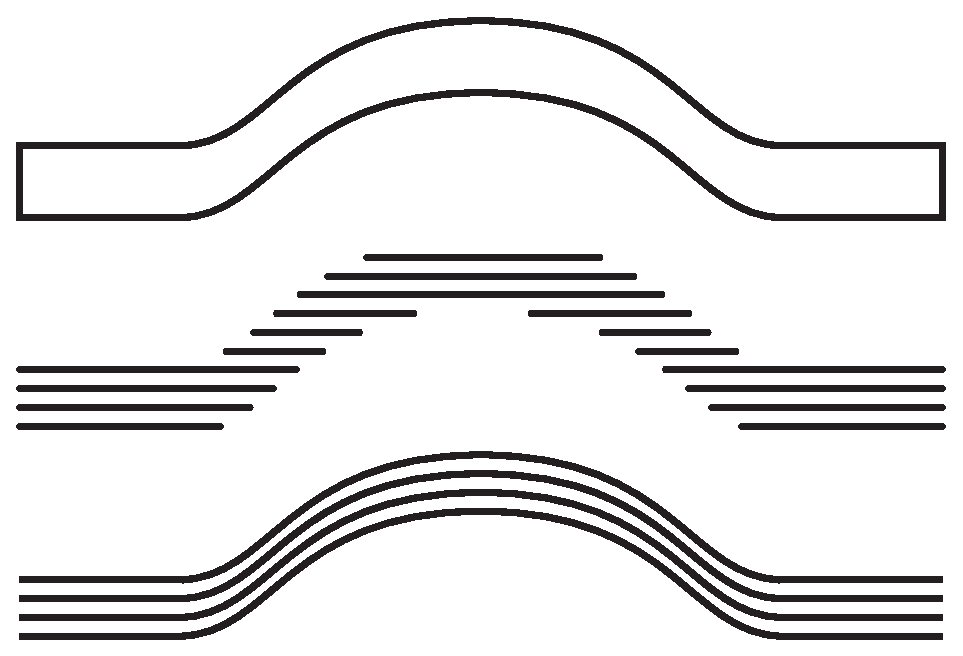
\includegraphics[width=0.5\textwidth]{./figures/layer-methods}
\caption{3D printing layer discretization methods. The desired part (top), typical planar/cartesian layers (middle), and curved layers (bottom).}
\label{fig:layers}
\end{figure}

To realize the goal of a fiber-reinforced composite curved layer 3D printer, the project was broken down into five subsystems, which are outlined in Figure~\ref{fig:flowchart}. First, all components of the 3D printing toolchain must be developed. The toolchain is defined by any hardware or software necessary for the steps between receiving a STereoLithography file (STL) and the printed part, which includes but is not limited to the extruder, control electronics, and the tool path generation scheme. Second, we must locate and learn to control a robot arm capable with six degrees of freedom. Third an appropriate CFRP with a usable ratio carbon fiber and thermoplastic matrix material is to be created. Fourth, computational and experimental methods can be utilized to determine optimal fiber orientation based on user requirements. Fifth, the printed parts will be experimental tests to quantify their mechanical properties. These five subsystems will come together to fully create the curved layer carbon fiber 3D printer.

\begin{figure}[htp]
\centering
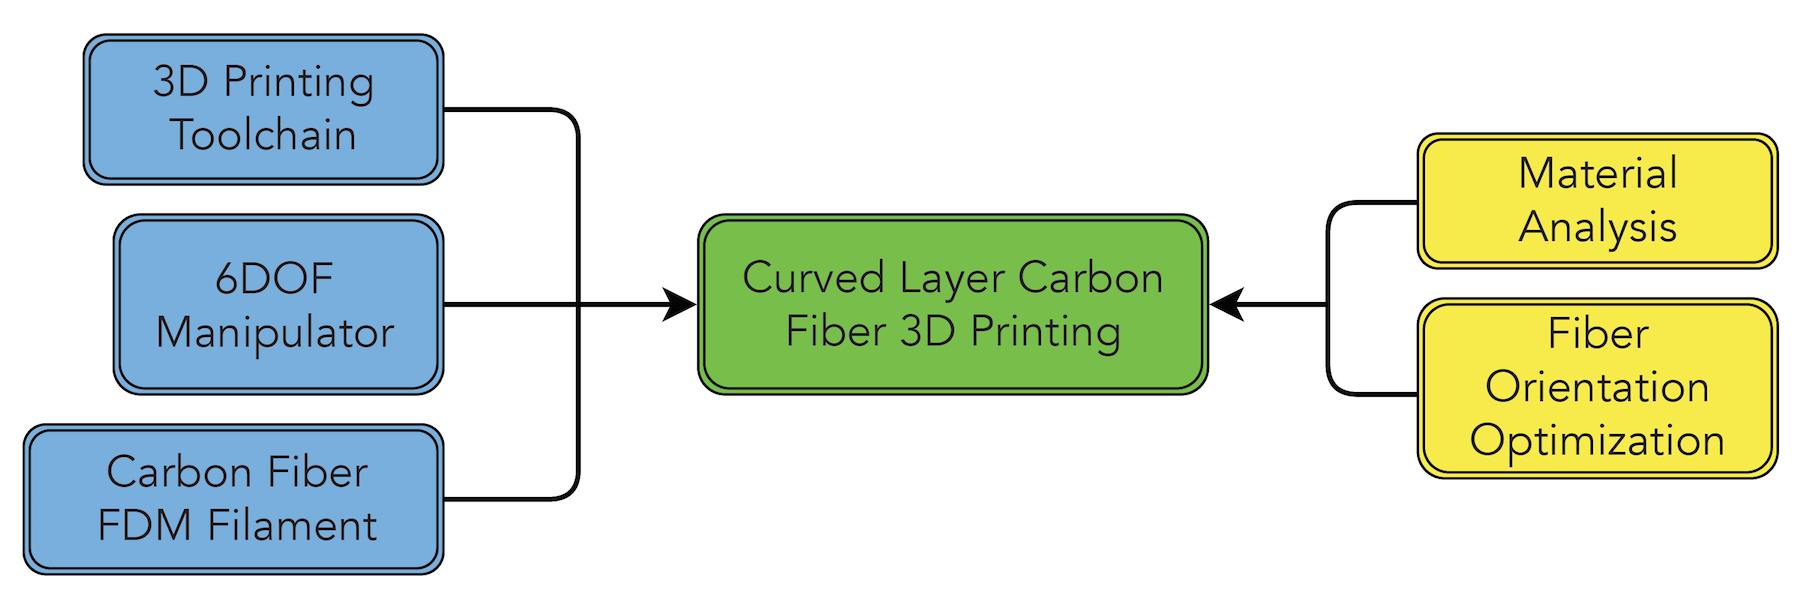
\includegraphics[width=0.75\textwidth]{./figures/flowchart}
\caption{A flow chart of subsystems.}
\label{fig:flowchart}
\end{figure}

%To realize the goal of a fiber-reinforced composite curved layer 3D printer, we will first learn to use to the FANUC LR Mate 200iC robot in The Cooper Union’s ME Rapid Prototyping Lab. This robot arm provides the necessary degrees of freedom for curved layer printing. We first plan to familiarize ourselves with the arm and control software by developing tool paths within its operational envelope. Then, we can mount an extruder to the arm and use an existing software toolchain to create standard flat-layer thermoplastic FDM prints. Once the standard print method is implemented, we can implement new gcode to create curved layer thermoplastic prints, while simultaneously investigating the best fiber composite to use as printing material. We will then alter the extruder mechanism to work with the chosen material. Finally, with curved layer fiber-reinforced 3D printing achieved, we plan to experimentally compare the mechanical strength of curved layer fiver-reinforced FDM prints to thermoplastic flat-layer FDM prints; the Instron machine in The Cooper Union’s ME Materials Lab can be used to load the parts and strain gauges can be attached to the parts to monitor specific local stresses.


%problem definition, background research, our project goal(s)

\clearpage

%----------------------------------------------------------
\section{3D Printing Toolchain}

\subsection{Extruder}

\indent

The extruder is the mechanism responsible for depositing the filament in a 3D printing system. Generally, this mechanism includes a motor that drives a gripping mechanism, which reels in and pushes the filament into a heated nozzle. The nozzle heats the filament to a soft state and lays the filament on the printing bed or on an already printed layer to create the part.\\

In the case of the curved layer carbon fiber 3D printer, the extruder is required to mount to the robot arm, be compact\footnote{The compact size is required for two reasons. First, to ensure that induced torque on the robot arm joints and gripper remain within safe operating conditions. Second, to readily permit the nozzle to deposit material when not perpendicular to the build platform, which will be required for printing curved layers.}, and accept filaments of a variety of sizes (likely ranging in diameter from 1.75 mm to 3 mm). \\

Figure~\ref{fig:old extruder} presents the initial design of the extruder in \emph{SolidWorks}. The extruder mounts to the Fanuc grippers and is constructed out of a combination of machined aluminum parts and RepRap hardware (nozzle, J-head, J-head mounting plate, ceramic heating element, thermistor, fan, and fan mount). This configuration locates the nozzle outlet along the mid-plane of the grippers for simple coordinate transformations when programming the robot to print. Laser-cut acrylic gears provide a 3:1 step up in torque from the stepper motor and drive a notched screw, which grips and pushes the filament into the nozzle. A bearing opposite the screw provides counter-pressure and its mounting plates can adjust the distance between the screw and bearing to accommodate different filament sizes.\\

\begin{figure}[h!]
\centering
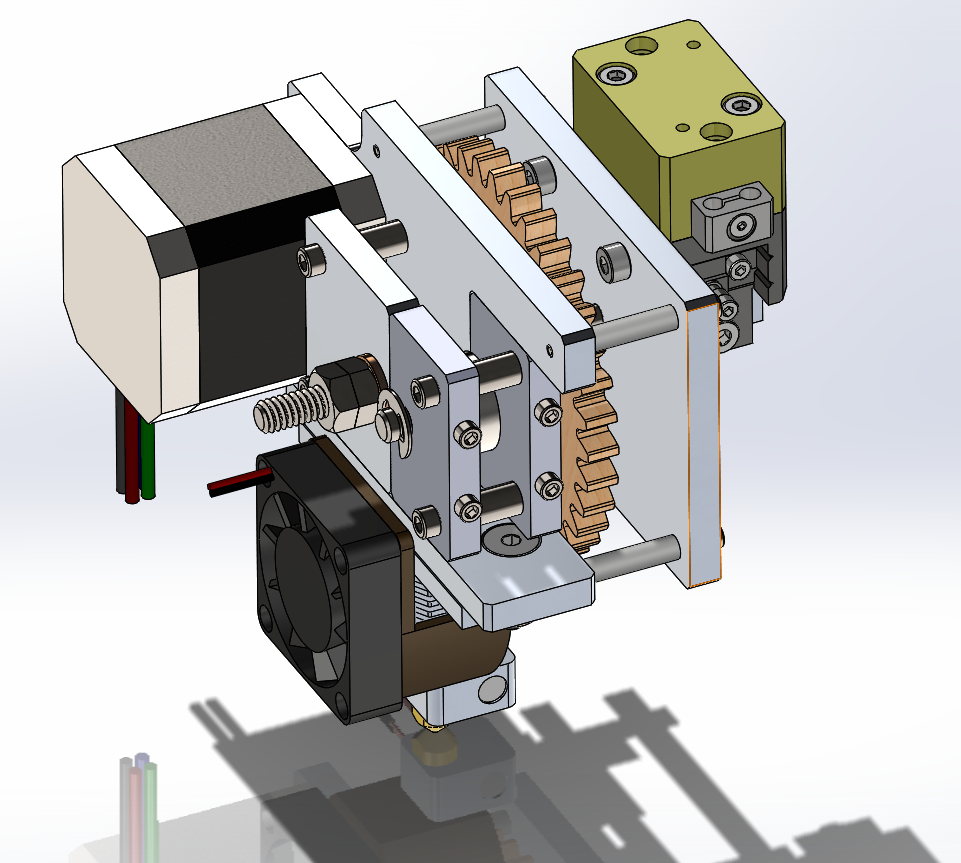
\includegraphics[width=0.5\textwidth]{./figures/extruder-old-2}
\caption{An isometric view of the initial extruder design.}
\label{fig:old extruder}
\end{figure}

To assess the feasibility of the initial extruder design, minor tweaks were implemented within the CAD to make a laser-cut prototype.  Figure~\ref{fig:prototype extruder} shows the prototype mounted on the FANUC grippers. The prototype served its purpose and demonstrated numerous problems with the initial design. There were some mis-measurements of RepRap hardware, using spacers instead of threaded standoffs decreased the rigidity of the structure, the structure was a bit larger than desired, and a few undetected interferences were discovered. Subsequently, the extruder then went through a series of redesigns to develop an acceptable configuration.\\

\begin{figure}[h!]
\centering
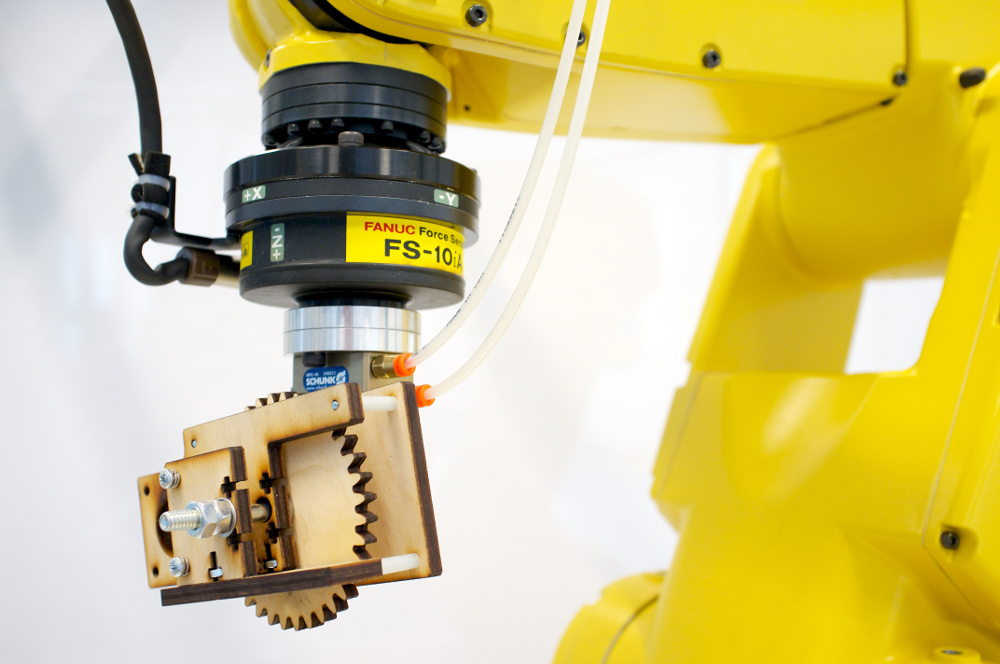
\includegraphics[width=0.5\textwidth]{./figures/extruder-prototype-2}
\caption{A photograph of the mounted prototype.}
\label{fig:prototype extruder}
\end{figure}

Figure~\ref{fig:extruder iso} presents a rendering of the final extruder design. Figure~\ref{fig:extruder drawing} provides general dimensions and annotations to fully present the extruder design concept. The final design is significantly smaller than the initial design, will require less machining, and uses less fastening hardware. The size decrease was accomplished by using smaller gears (50\% scaled versions of gears dimensions taken from \emph{SDP-SI}\footnote{\url{http://www.sdp-si.com/}} and located the stepper motor directly beneath the FANUC grippers. As part of the design process the gears were laser-cut, and physically tested to ensure that the teeth would not shear off under a load less than the stall torque of the stepper motor, before being fully committed to this design. The stepper motor (Sparkfun ROB-10846) outputs 68 oz-in of torque and has a resolution of 400 steps/revolution. Two laser-cut acrylic gears step up the torque to 204 oz-in.\footnote{Most extruders in the 3D printing community use analogous stepper motors and utilize gear trains to step up the torque. Common gear ratios range from 2:1 to 4:1 depending on the specific qualities of the filament. Given that the specifics of the filament are not yet fully determined, the mean value was used.} A partially threaded screw will be notched on the mill to contain teeth-like features along a portion of its length. These teeth will grip the filament and push it into the extruder. The screw rides along two bronze PTFE-coated bearings to ensure smooth rotation during printing. Two adjustment plates locate a bearing just opposite the screw to provide counter-pressure during printing. The plates are secured in place using four screws, which can be loosened or tightened to adjust the distance between the screw and bearing to accommodate different filament sizes. Shims or spring washers may have to be utilized to located this adjustable mechanism in its optimal position for the official CFRP.\\

The extruder will be machined with aluminum to provide rigidity. Many 3D printers utilize 3D printed bodies for mounting RepRap hardware, but the associated poor tolerances and material flexibility are not ideal for the curved layer carbon fiber 3D printer. Machining the extruder out of aluminum will allow easy implementation of any future adjustments and ensures all mechanisms will align properly. The entire extruder assembly secures to the FANUC gripper with four screws.\\

\begin{figure}[h!]
\centering
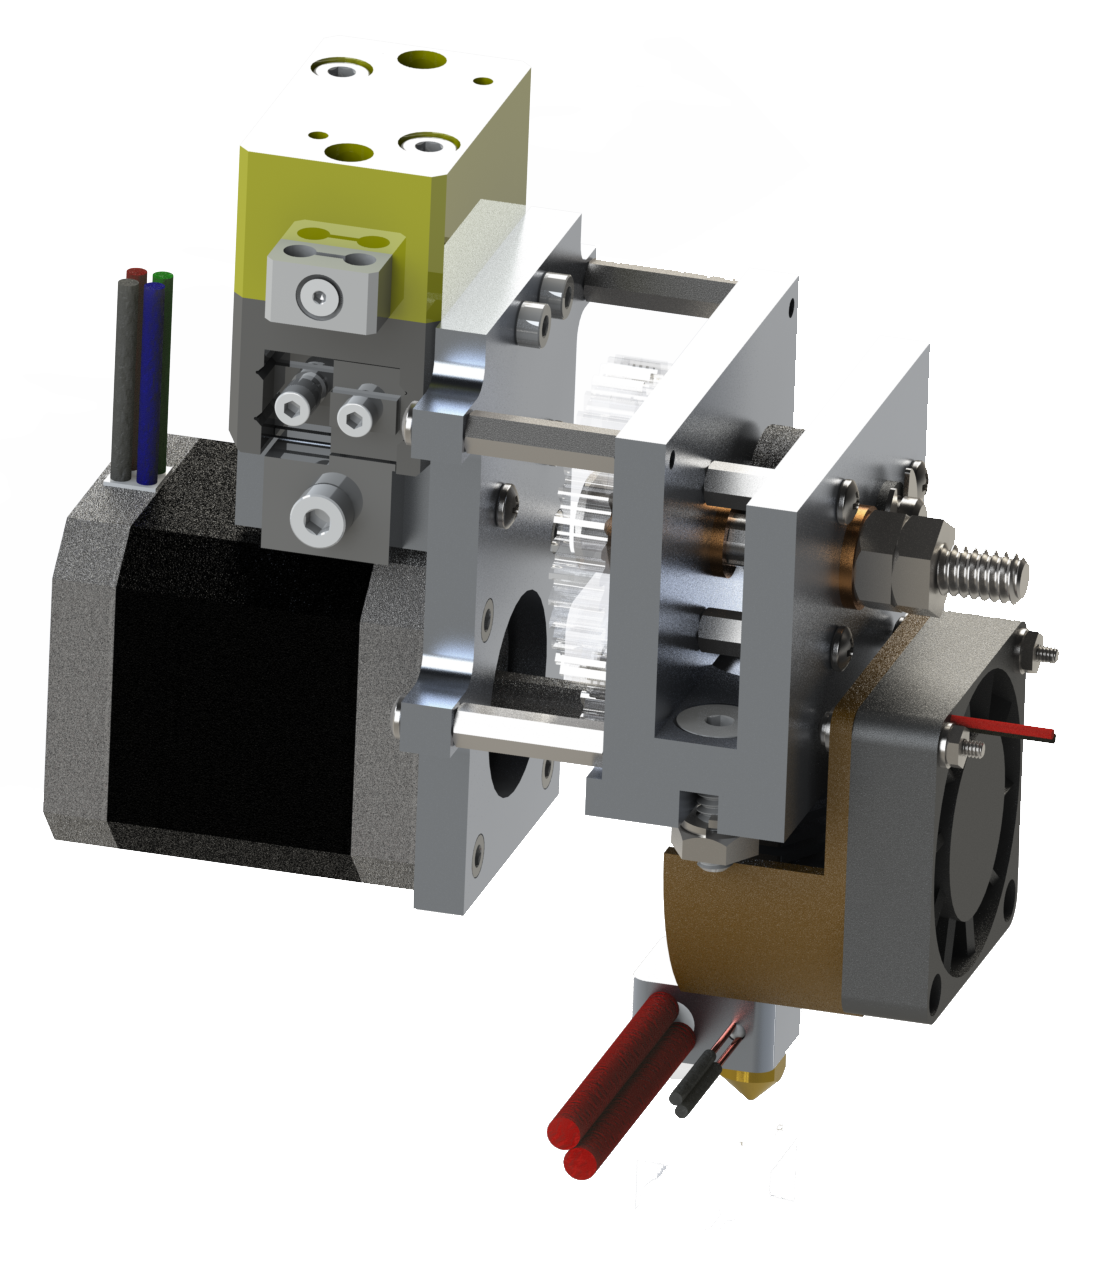
\includegraphics[width=0.5\textwidth]{./figures/extruder-iso}
\caption{An isometric render of the final extruder design.}
\label{fig:extruder iso}
\end{figure}

\begin{figure}[h!]
\centering
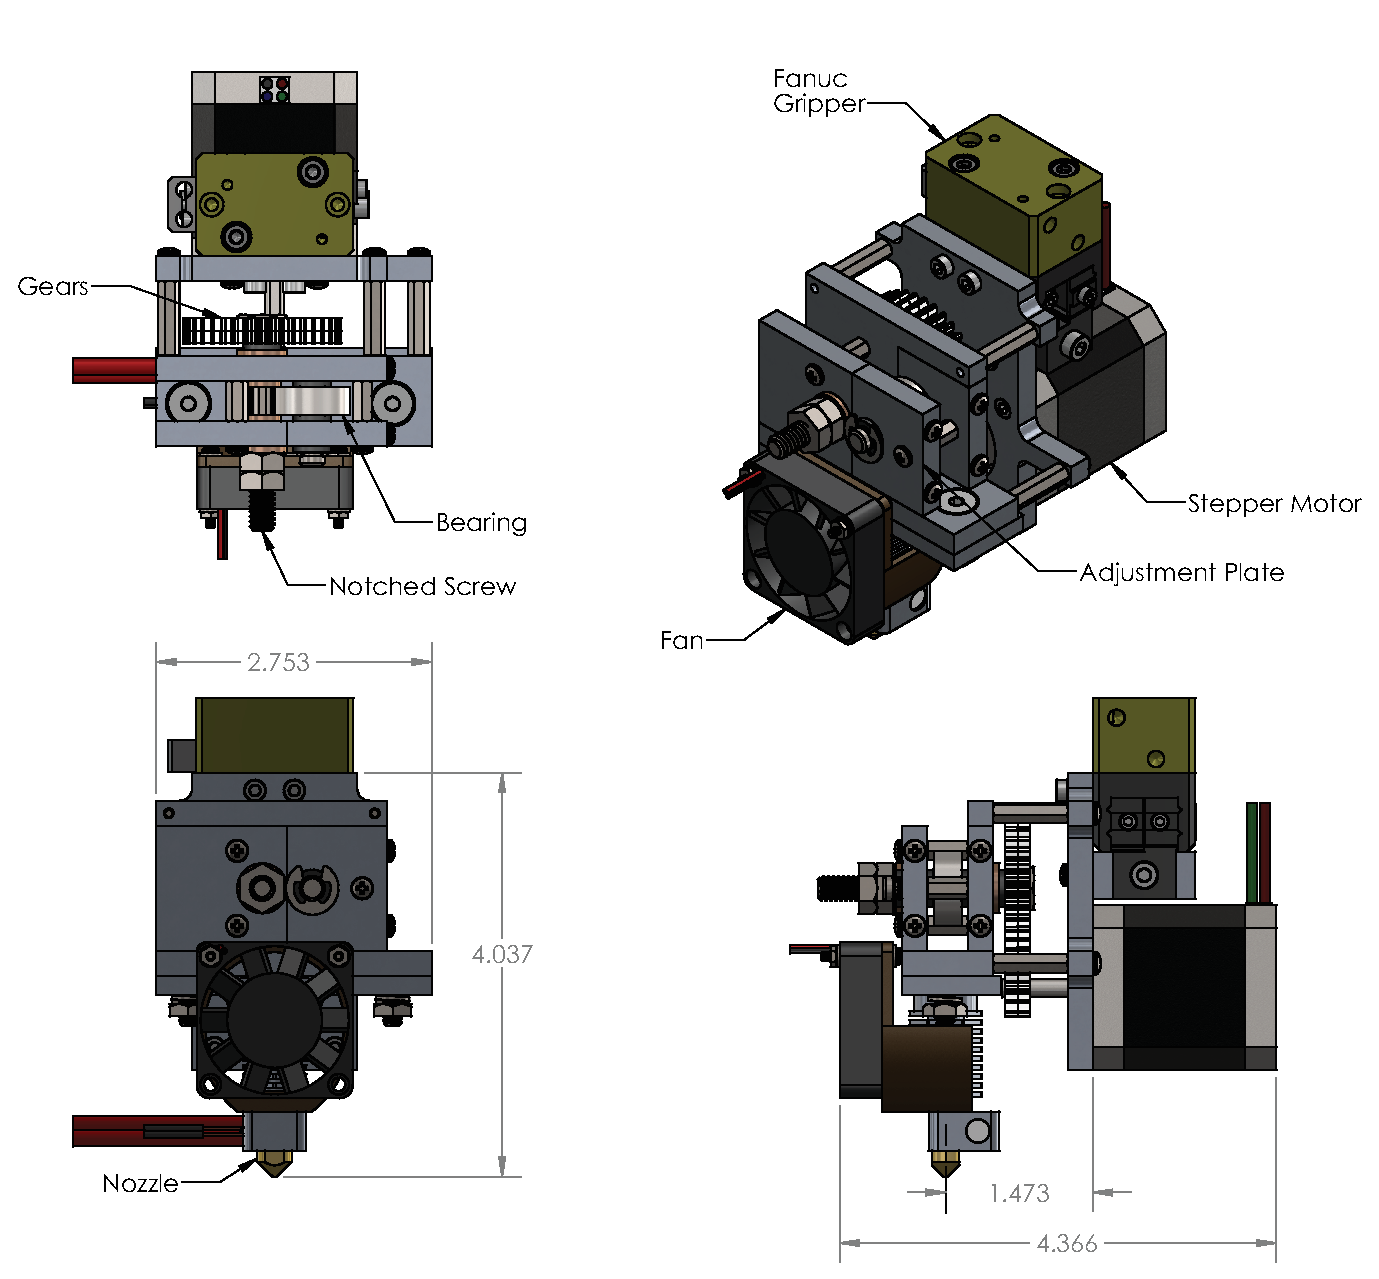
\includegraphics[width=1\textwidth]{./figures/extruder-drawing}
\caption{A general drawing of the final extruder design.}
\label{fig:extruder drawing}
\end{figure}

\clearpage




\subsection{Control Electronics}

\indent 

The extruder is controlled by a Megatronics control board, shown in Figure~\ref{fig:megatronics}, which was developed for the RepRap open source 3D printer project. The board contains all the necessary electronics to drive a Cartesian coordinate based FDM desktop 3D printer. The board can drive numerous positioning and extruder motors, heating elements, sensors, displays, and more. Because the FANUC robot handles the extruder positioning, the Megatronics board will be used to control the extruder elements only.\\

\begin{figure}[htp]
\centering
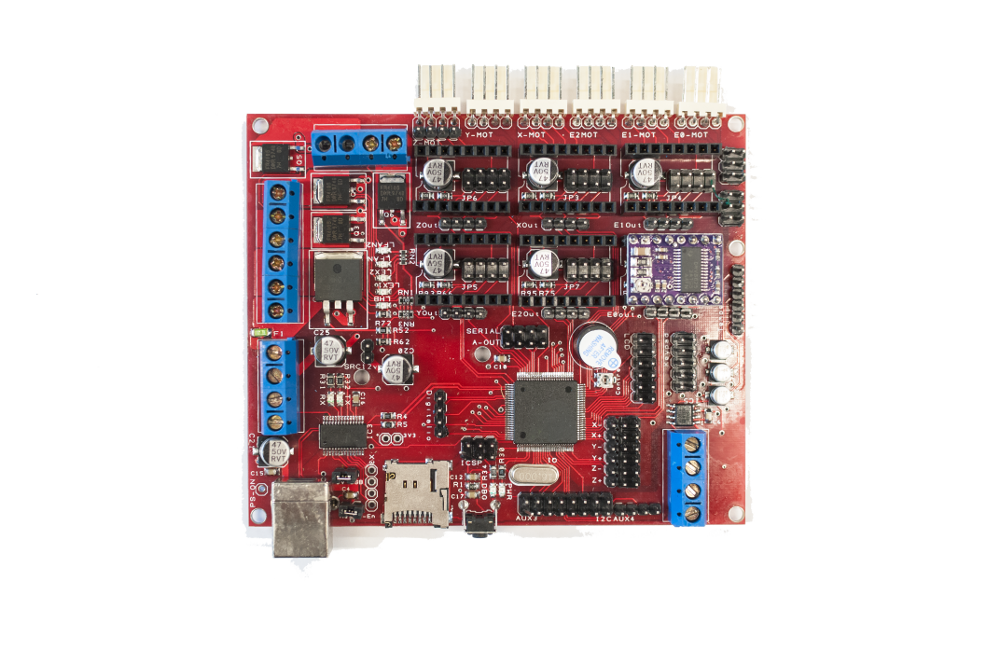
\includegraphics[width=0.5\textwidth]{./figures/electronics-board}
\caption{A photo of the Megatronics Control Board.}
\label{fig:megatronics}
\end{figure}

\subsubsection{Firmware}

\indent

When used in RepRap printers, the Megatronics board is typically used with one of several open source firmwares that are also associated with the RepRap project. Because these firmwares were designed with Cartesian desktop FDM printers in mind, they work well with the Megatronics board. The chosen firmware is uploaded to the board using a USB cable. For the FANUC-mounted extruder, a suitable firmware will be chosen and modified to work with the FANUC robot.\\

The firmware will be modified to control only the components present on the FANUC-mounted extruder. The firmware's timing functions must be modified as well. Normally, the firmware calculates its own filament feed rates and motor speeds in order to ensure that the flow rate of the extruded material follows the surface speed of the extruder with respect to the print surface. Because the FANUC controller has its own closed-loop control and is much less flexible than the RepRap firmware, the firmware will be modified to monitor the FANUC robot speed and position, and act accordingly. The monitoring will be accomplished by polling robot status system variables from a digital output on the FANUC controller.

\subsubsection{Enclosure}

\indent

The Megatronics board is too large to be mounted directly to the extruder, so it has been mounted inside the FANUC robot cage. The board is housed in a clear acrylic housing, shown in Figures~\ref{fig:megatronics-mount-back} and \ref{fig:megatronics-mount-front}, which serves several purposes. The housing protects the board from debris and accidental touches by either people or by the robot. The clear front makes the on-board status LEDs visible for debugging and operation. The back of the housing has built-in slots that provide anchors for cable management hardware. The cable management hardware will both organize the wires connected to the board and provide strain relief. The strain relief is especially important for the wires that connect the board and the extruder, because they will move with the extruder. The housing is positioned in a location that will cause the least interference between the wires and the arm. The power and USB cables for the board will be routed through the robot cage members. The USB cable will provide convenient access for updating the board firmware and collecting data using a laptop. 

\begin{figure}[htp]
\centering
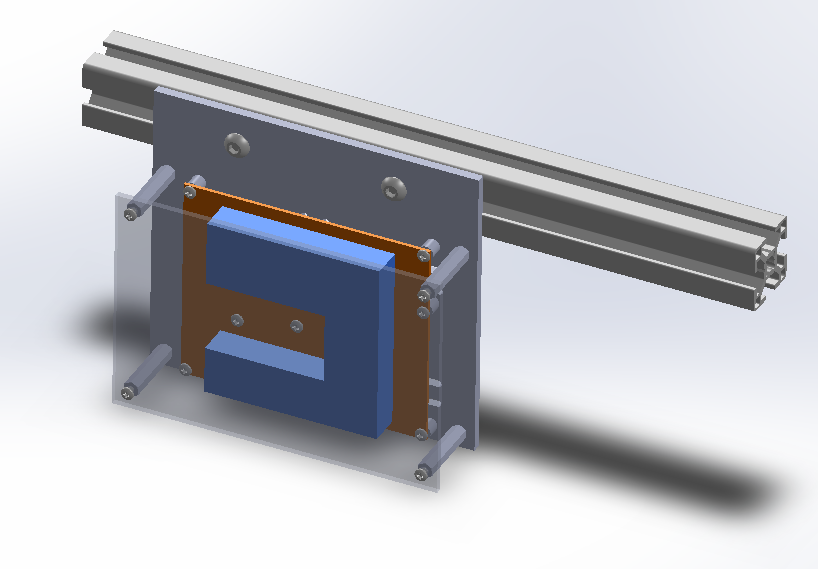
\includegraphics[width=0.5\textwidth]{./figures/megatronics-mount-1}
\caption{A \emph{SolidWorks} model of the mounted Megatronics board.}
\label{fig:megatronics-mount-back}
\end{figure}

\begin{figure}[htp]
\centering
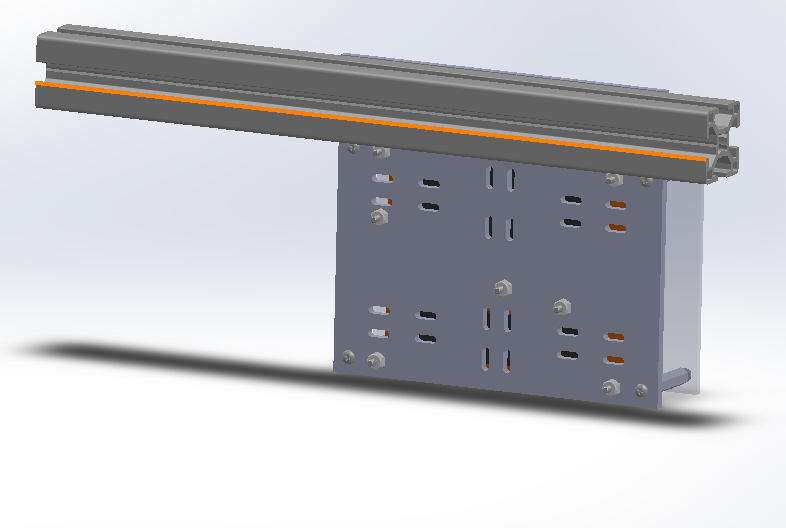
\includegraphics[width=0.5\textwidth]{./figures/megatronics-mount-2}
\caption{A \emph{SolidWorks} model of the mounted Megatronics board.}
\label{fig:megatronics-mount-front}
\end{figure}




%extruder, control electronics, slicing algorithm & layer generation

\clearpage

%----------------------------------------------------------
\section{6 Degree of Freedom Manipulator}

\indent

To extrude a consistent bead of material along a surface, the extruder nozzle should be normal to the surface. This means that in flat layer printing, the extruder may always be held vertically above the print surface. However, curved layers may require the extruder to tilt and rotate to reach some areas properly. Thus, curved layer FDM 3D printing requires the extruder positioning mechanism to have more degrees of freedom than flat-layer printing. \\

The FANUC LR Mate 200iC 6 degree of freedom industrial robot arm provides the necessary degrees of freedom for curved layer printing. The robot was acquired as part of an eductional package that includes the robot, its housing, the controller, a gripper and vision system, and related softwrae. The robot is compact and has positioning repeatable to 0.02 mm. As such, the robot is a suitable platform for a curved layer 3D printer. The extruder will be mounted to the existing gripper, and the control electronics and filament will be mounted to the side of the robot cage. Figure~\ref{fig:robot} provides a photograph of the FANUC robot itself, while Figure~\ref{fig:robot with things} shows a photograph of the FANUC with the electronics board and extruder.\\

%% talk about speed / position tracking and built in language?

\begin{figure}[htp]
\centering
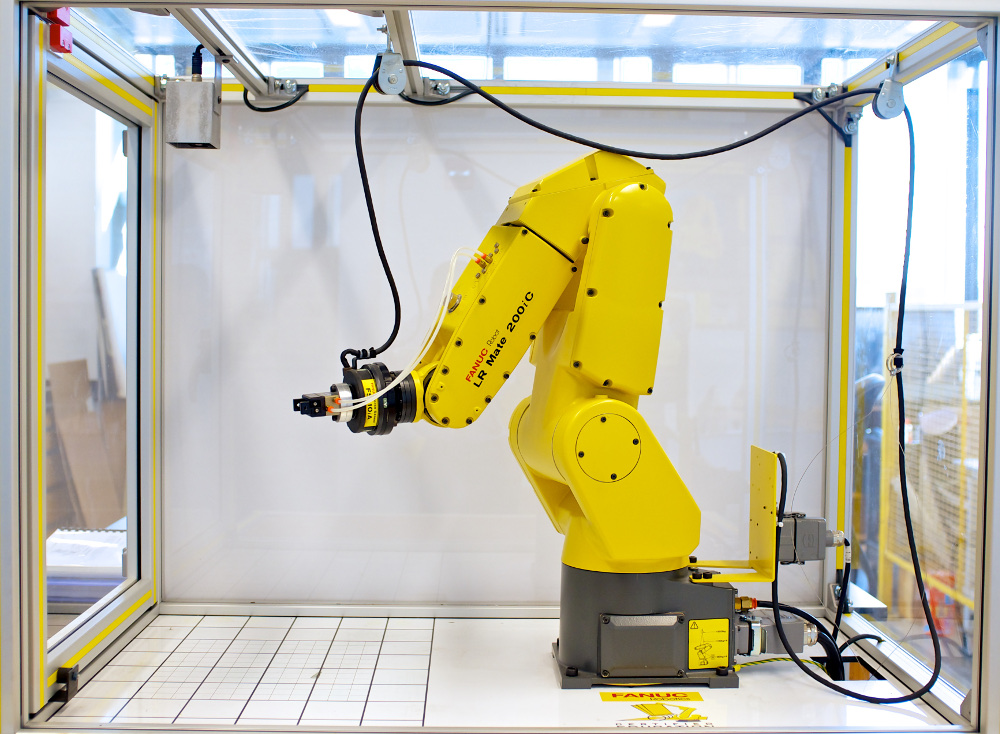
\includegraphics[width=0.5\textwidth]{./figures/robot}
\caption{A photograph of the FANUC LR Mate 200iC robot arm inside its cage.}
\label{fig:robot}
\end{figure}

\begin{figure}[htp]
\centering
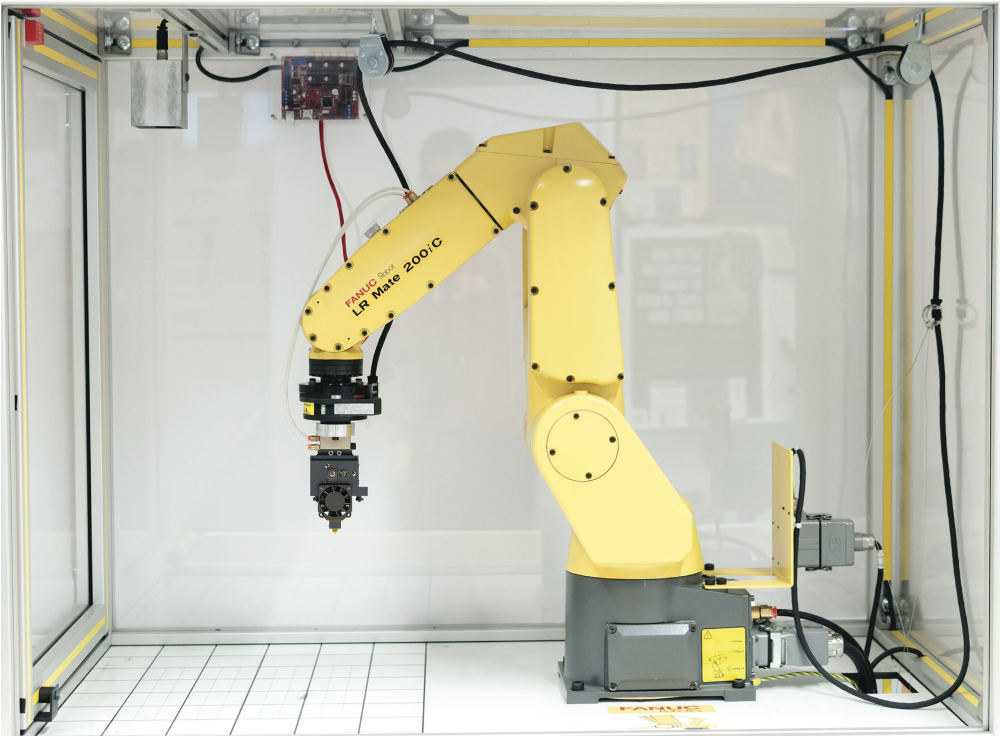
\includegraphics[width=0.5\textwidth]{./figures/robot-extruder-electronics}
\caption{A photograph of the robot with the mounted electronics and a rendering of the extruder.}
\label{fig:robot with things}
\end{figure}

%robots

\clearpage

%----------------------------------------------------------
\section{Carbon Fiber Filament}

\indent

In order to print the CFRP material, carbon fiber and a resin were combined into a CFRP filament. As in conventional FDM printing, the CFRP filament is extruded by driving it through a heated nozzle. ABS plastic was chosen as the matrix material for this filament for several reasons. First, ABS has already successfully been combined with chopped carbon fiber in FDM filaments. Second, ABS does not require post-processing to reach full strength, as epoxy-based pre-impregnated carbon fiber composites do. In all filament development methods a 1K carbon fiber tow (shown in Figure~\ref{fig:carbon-fiber-spool}) was utilized.\\

\begin{figure}[htp]
    \centering
    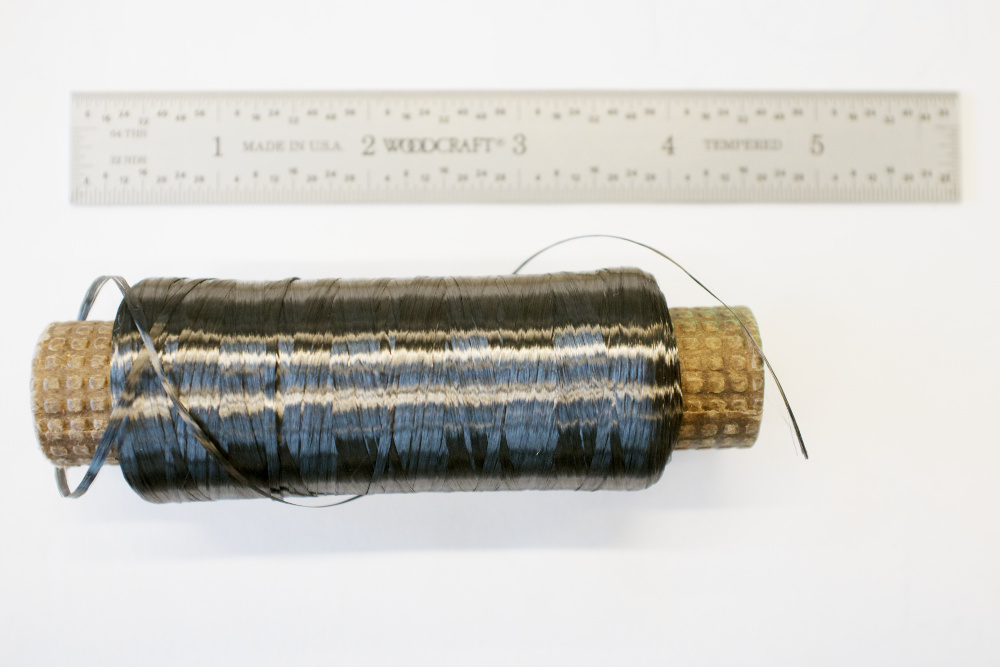
\includegraphics[width=0.5\textwidth]{./figures/carbon-fiber-spool}
    \caption{The 1K carbon fiber spool.}
    \label{fig:carbon-fiber-spool}
\end{figure}

\subsection{Production Methods}

\indent

Two proudction methods were explored for developing a CFRP filament. The first was pultrusion, an efficient fabrication method widely used to manufacture fiber-reinforced structural members. The second was a slurry dipping method, a tedious process where fibers were guided through a solution containing ABS, which would air dry onto the fibers and provide full fiber wet-out.\\

\subsubsection{Pultrusion}

\indent

A 3Doodler handheld 3D printing device was employed in pultrusion tests. The 3Doodler's feed motor was disabled, and then a bundle of carbon fiber and an ABS rod were simultaneously fed through the 3Doodler's heater and nozzle. The combined materials were manually drawn through from the exit end of the nozzle. This process is shown in Figure~\ref{fig:pultrusion-vid}. In the resulting filament, the carbon fiber bundle and the ABS adhered together well. However, due to the high viscosity of the heated ABS, most of the individual carbon fibers were not in contact with the ABS. Additionally, the fiber is not centered within the new CFRP filament, which is necessary printing.\footnote{Fibers located on the outside of the CFRP filament encounter a no-slip condition when entering the heated nozzle and subsequently never leave the nozzle with the ABS.} This effect is visible in Figure~\ref{fig:pultruded-scope}.\\

\begin{figure}[h!]
    \centering
    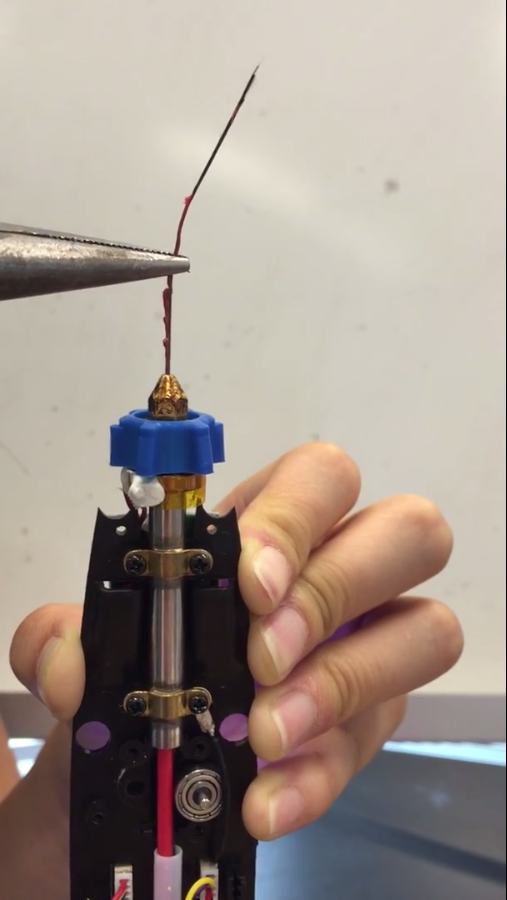
\includegraphics[width=0.4\textwidth]{./figures/pultrusion-vid}
    \caption{The experimental pultrusion setup, using the 3Doodler.}
    \label{fig:pultrusion-vid}
\end{figure}

\begin{figure}[h!]
    \centering
    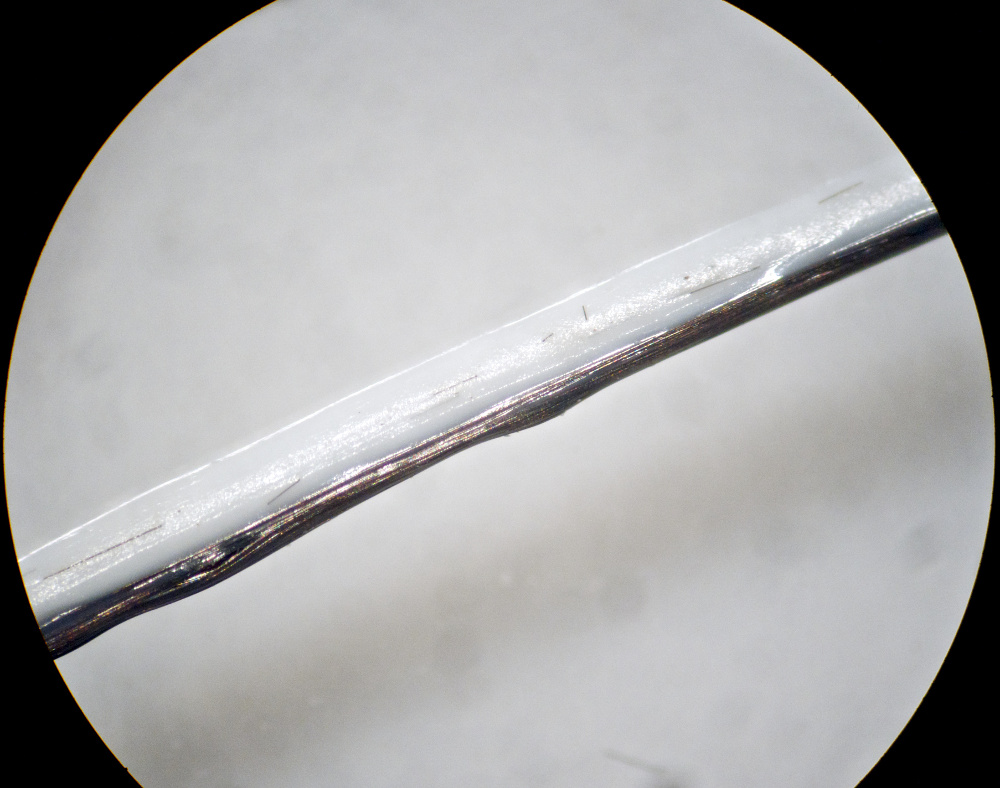
\includegraphics[width=0.6\textwidth]{./figures/pultruded-scope}
    \caption{Pultruded filament sample, magnified 10x under a microscope.}
    \label{fig:pultruded-scope}
\end{figure}

\clearpage

\subsubsection{Slurry Dipping}

Good fiber wet-out is critical to the performance of fiber composites, so another filament production method was explored. In the new procedure, achieving complete wet-out was prioritized. ABS plastic was dissolved in acetone to make a slurry. A fiber guide was fabricated to guide the carbon fiber in and out of the slurry. Carbon fiber bundles were then drawn through the fiber guide and allowed to dry. The process setup is shown in Figure~\ref{fig:dipping-vid}. As the acetone evaporated from the slurry, a small amount of ABS was left on the carbon fibers. The resulting filament showed very good wet-out. A pultruded sample and a dipped sample are shown side-by-side in Figure~\ref{fig:two-samples}.\\

\begin{figure}[h!]
    \centering
    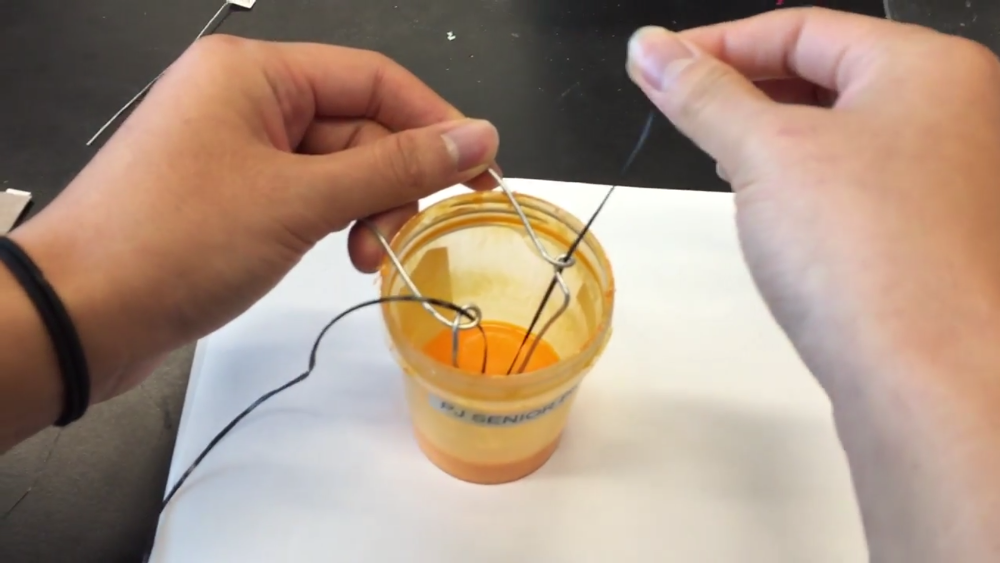
\includegraphics[width=0.8\textwidth]{./figures/dipping-vid}
    \caption{The basic slurry dipping process.}
    \label{fig:dipping-vid}
\end{figure}

\begin{figure}[h!]
    \centering
    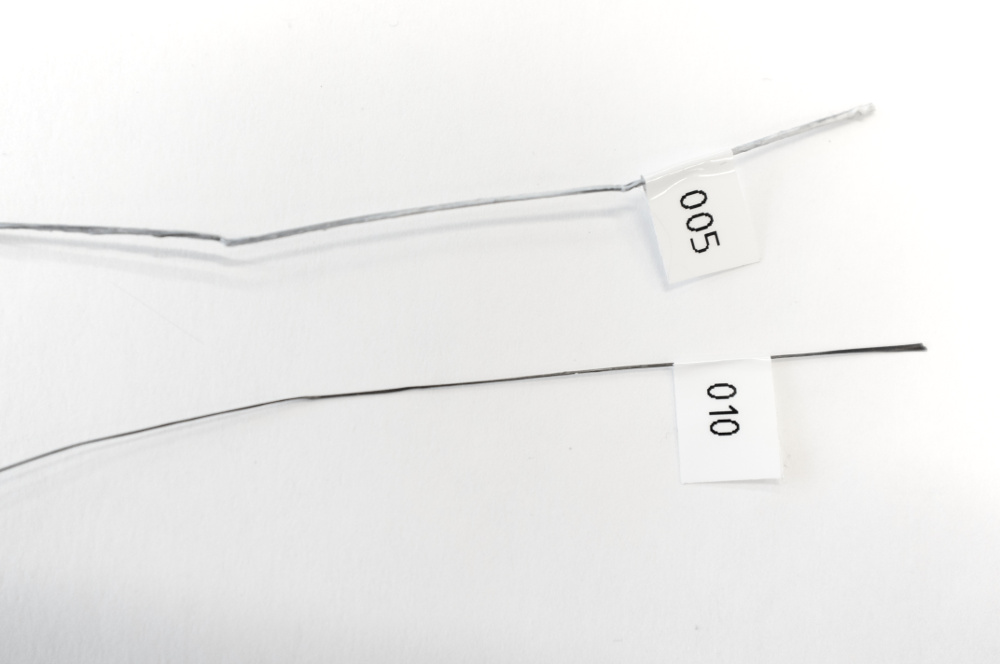
\includegraphics[width=0.6\textwidth]{./figures/FilamentSample}
    \caption{A pultruded filament sample (top) and a dipped filament sample (bottom), labeled with sample numbers.}
    \label{fig:two-samples}
\end{figure}

As the more promising of the two methods, dipping was explored further in attempt to create a viable CFRP filament.\\

%%% Slurry Photos



%%% Dipping Method Diagrams

%\begin{figure}[h!]
%    \centering
%    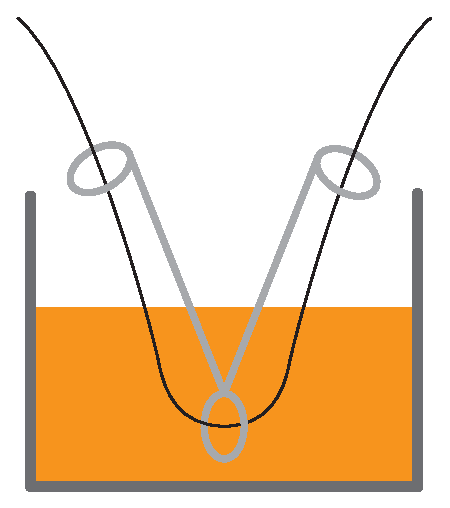
\includegraphics[width=0.5\textwidth]{./figures/external-dip-diagram}
%    \caption{An illustration of a wire-guided dipping method with the guide only partially immersed in the slurry.}
%    \label{fig:external-dip-diagram}
%\end{figure}
%
%\begin{figure}[h!]
%    \centering
%    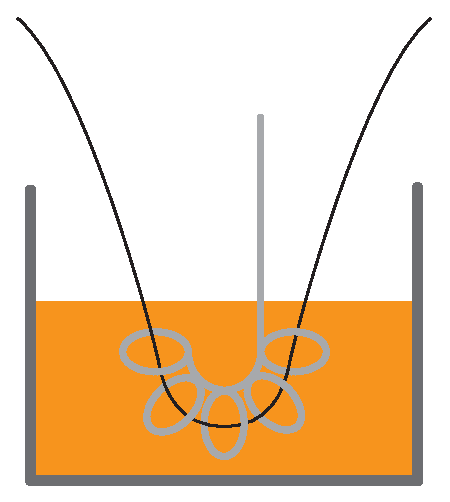
\includegraphics[width=0.5\textwidth]{./figures/internal-dip-diagram}
%    \caption{An illustration of a wire-guided dipping method with the guide fully immersed in the slurry.}
%    \label{fig:internal-dip-diagram}
%\end{figure}
%
%\begin{figure}[h!]
%    \centering
%    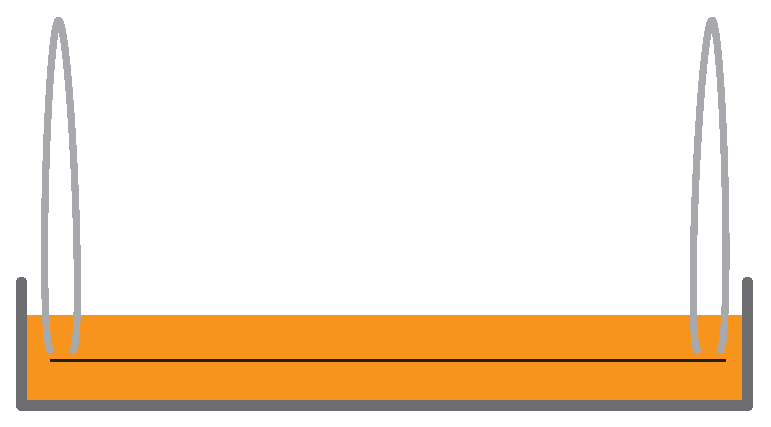
\includegraphics[width=0.5\textwidth]{./figures/flat-dip-diagram}
%    \caption{An illustration of the bath dipping method.}
%    \label{fig:flat-dip-diagram}
%\end{figure}

\begin{figure}[h!]
        \centering
        \begin{subfigure}[b]{0.3\textwidth}
                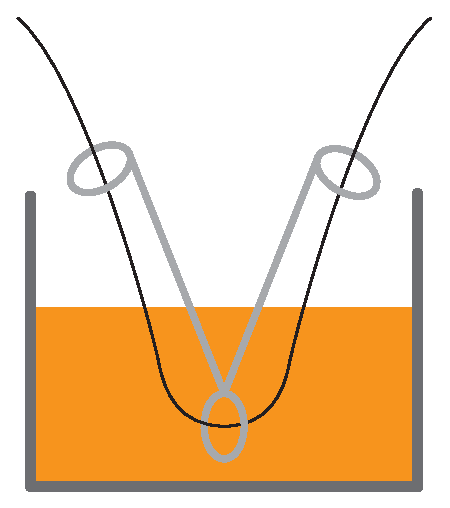
\includegraphics[width=\textwidth]{./figures/external-dip-diagram}
                \caption{Partially immersed guide.}
                \label{fig:external-dip-diagram}
        \end{subfigure}%
        ~ %add desired spacing between images, e. g. ~, \quad, \qquad, \hfill etc.
          %(or a blank line to force the subfigure onto a new line)
        \begin{subfigure}[b]{0.3\textwidth}
                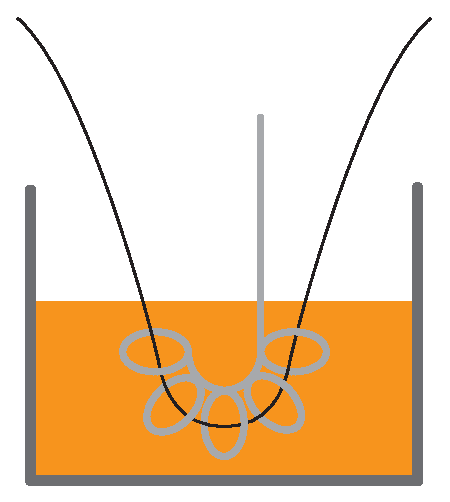
\includegraphics[width=\textwidth]{./figures/internal-dip-diagram}
                \caption{Fully immersed guide.}
                \label{fig:internal-dip-diagram}
        \end{subfigure}
        ~ %add desired spacing between images, e. g. ~, \quad, \qquad, \hfill etc.
          %(or a blank line to force the subfigure onto a new line)
        \begin{subfigure}[b]{0.3\textwidth}
                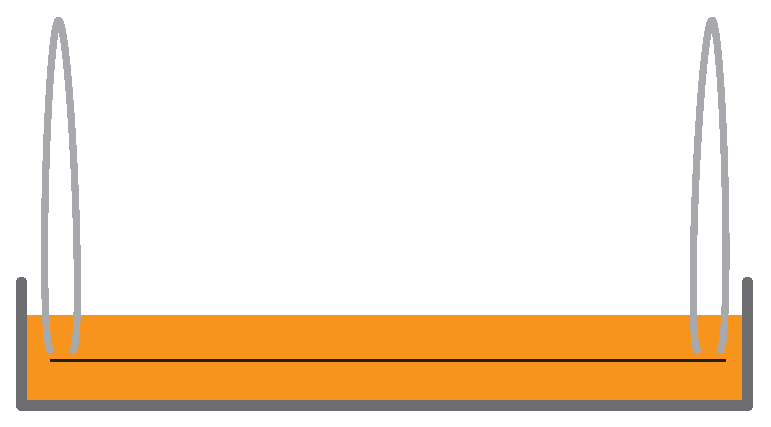
\includegraphics[width=\textwidth]{./figures/flat-dip-diagram}
                \caption{Bath dipping.}
                \label{fig:flat-dip-diagram}
        \end{subfigure}
        \caption{Slurry Dippng Methods.}\label{fig:dip-diagram}
\end{figure}

%%% slurry making photos

\begin{figure}[h!]
        \centering
        \begin{subfigure}[b]{0.3\textwidth}
                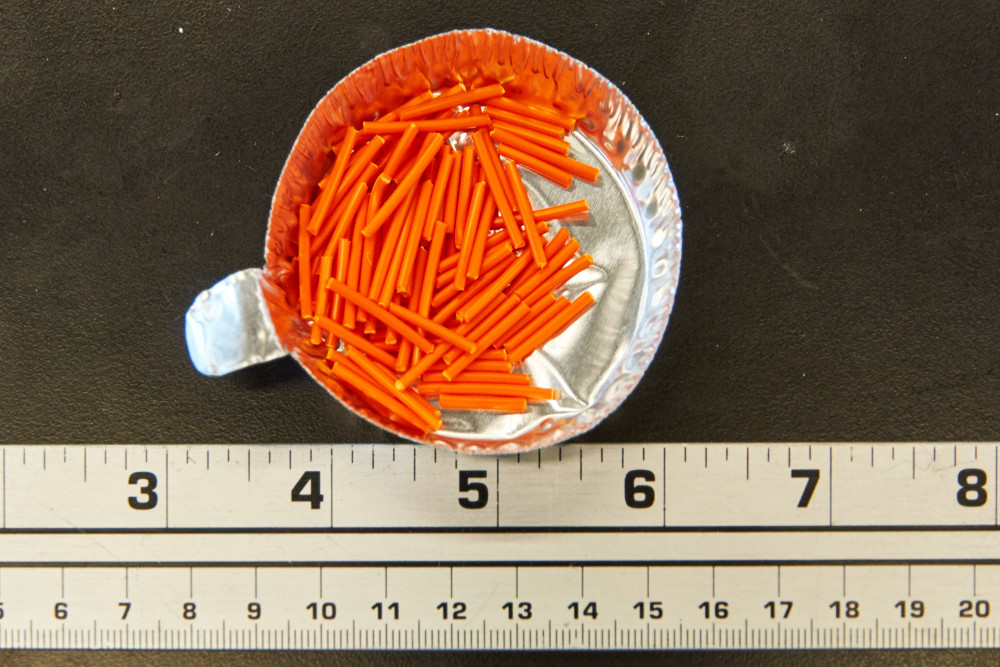
\includegraphics[width=\textwidth]{./figures/filament-abs-chopped}
                \caption{Chopped ABS.}
                \label{fig:filament-abs-chopped}
        \end{subfigure}%
        \begin{subfigure}[b]{0.3\textwidth}
                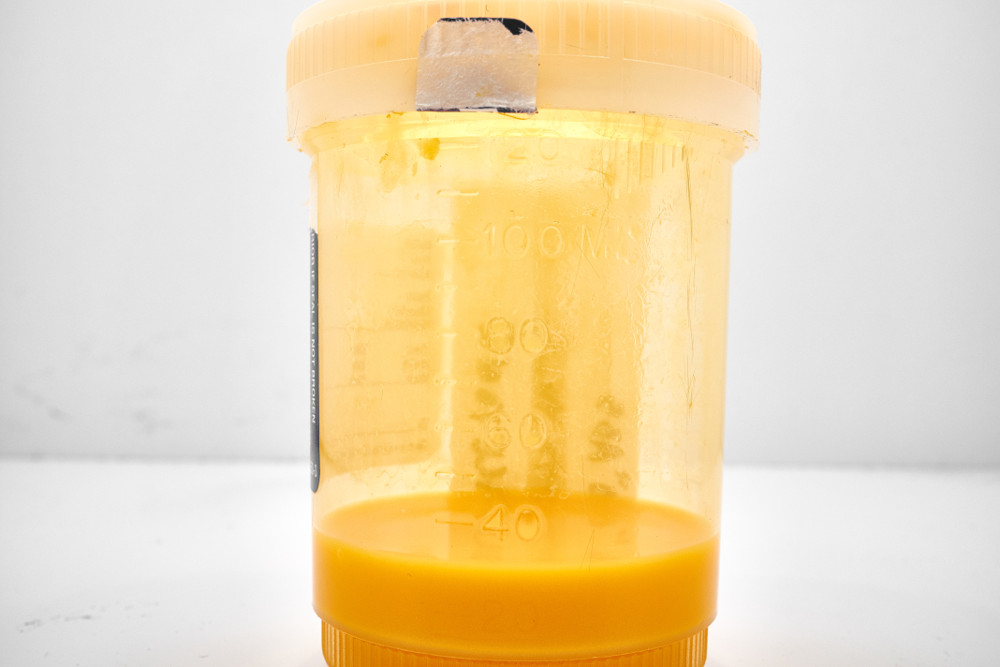
\includegraphics[width=\textwidth]{./figures/filament-mixture-volume-markings}
                \caption{Various mixtures.}
                \label{fig:filament-mixture-volume-markings}
        \end{subfigure}
        \begin{subfigure}[b]{0.3\textwidth}
                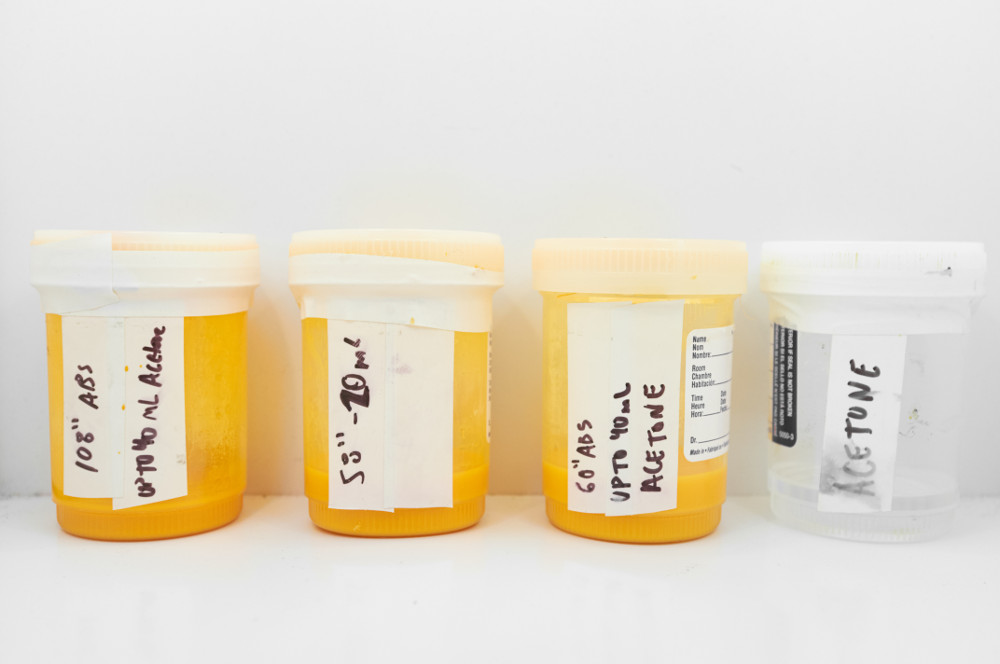
\includegraphics[width=\textwidth]{./figures/filament-mixtures}
                \caption{Volume markings.}
                \label{fig:filament-mixtures}
        \end{subfigure}
        \caption{Photos of the ABS-acetone slurry-making process}\label{fig:slurry-making}
\end{figure}

%%% Filament Photos

% external guide

\begin{figure}[h!]
        \centering
        \begin{subfigure}[b]{0.3\textwidth}
                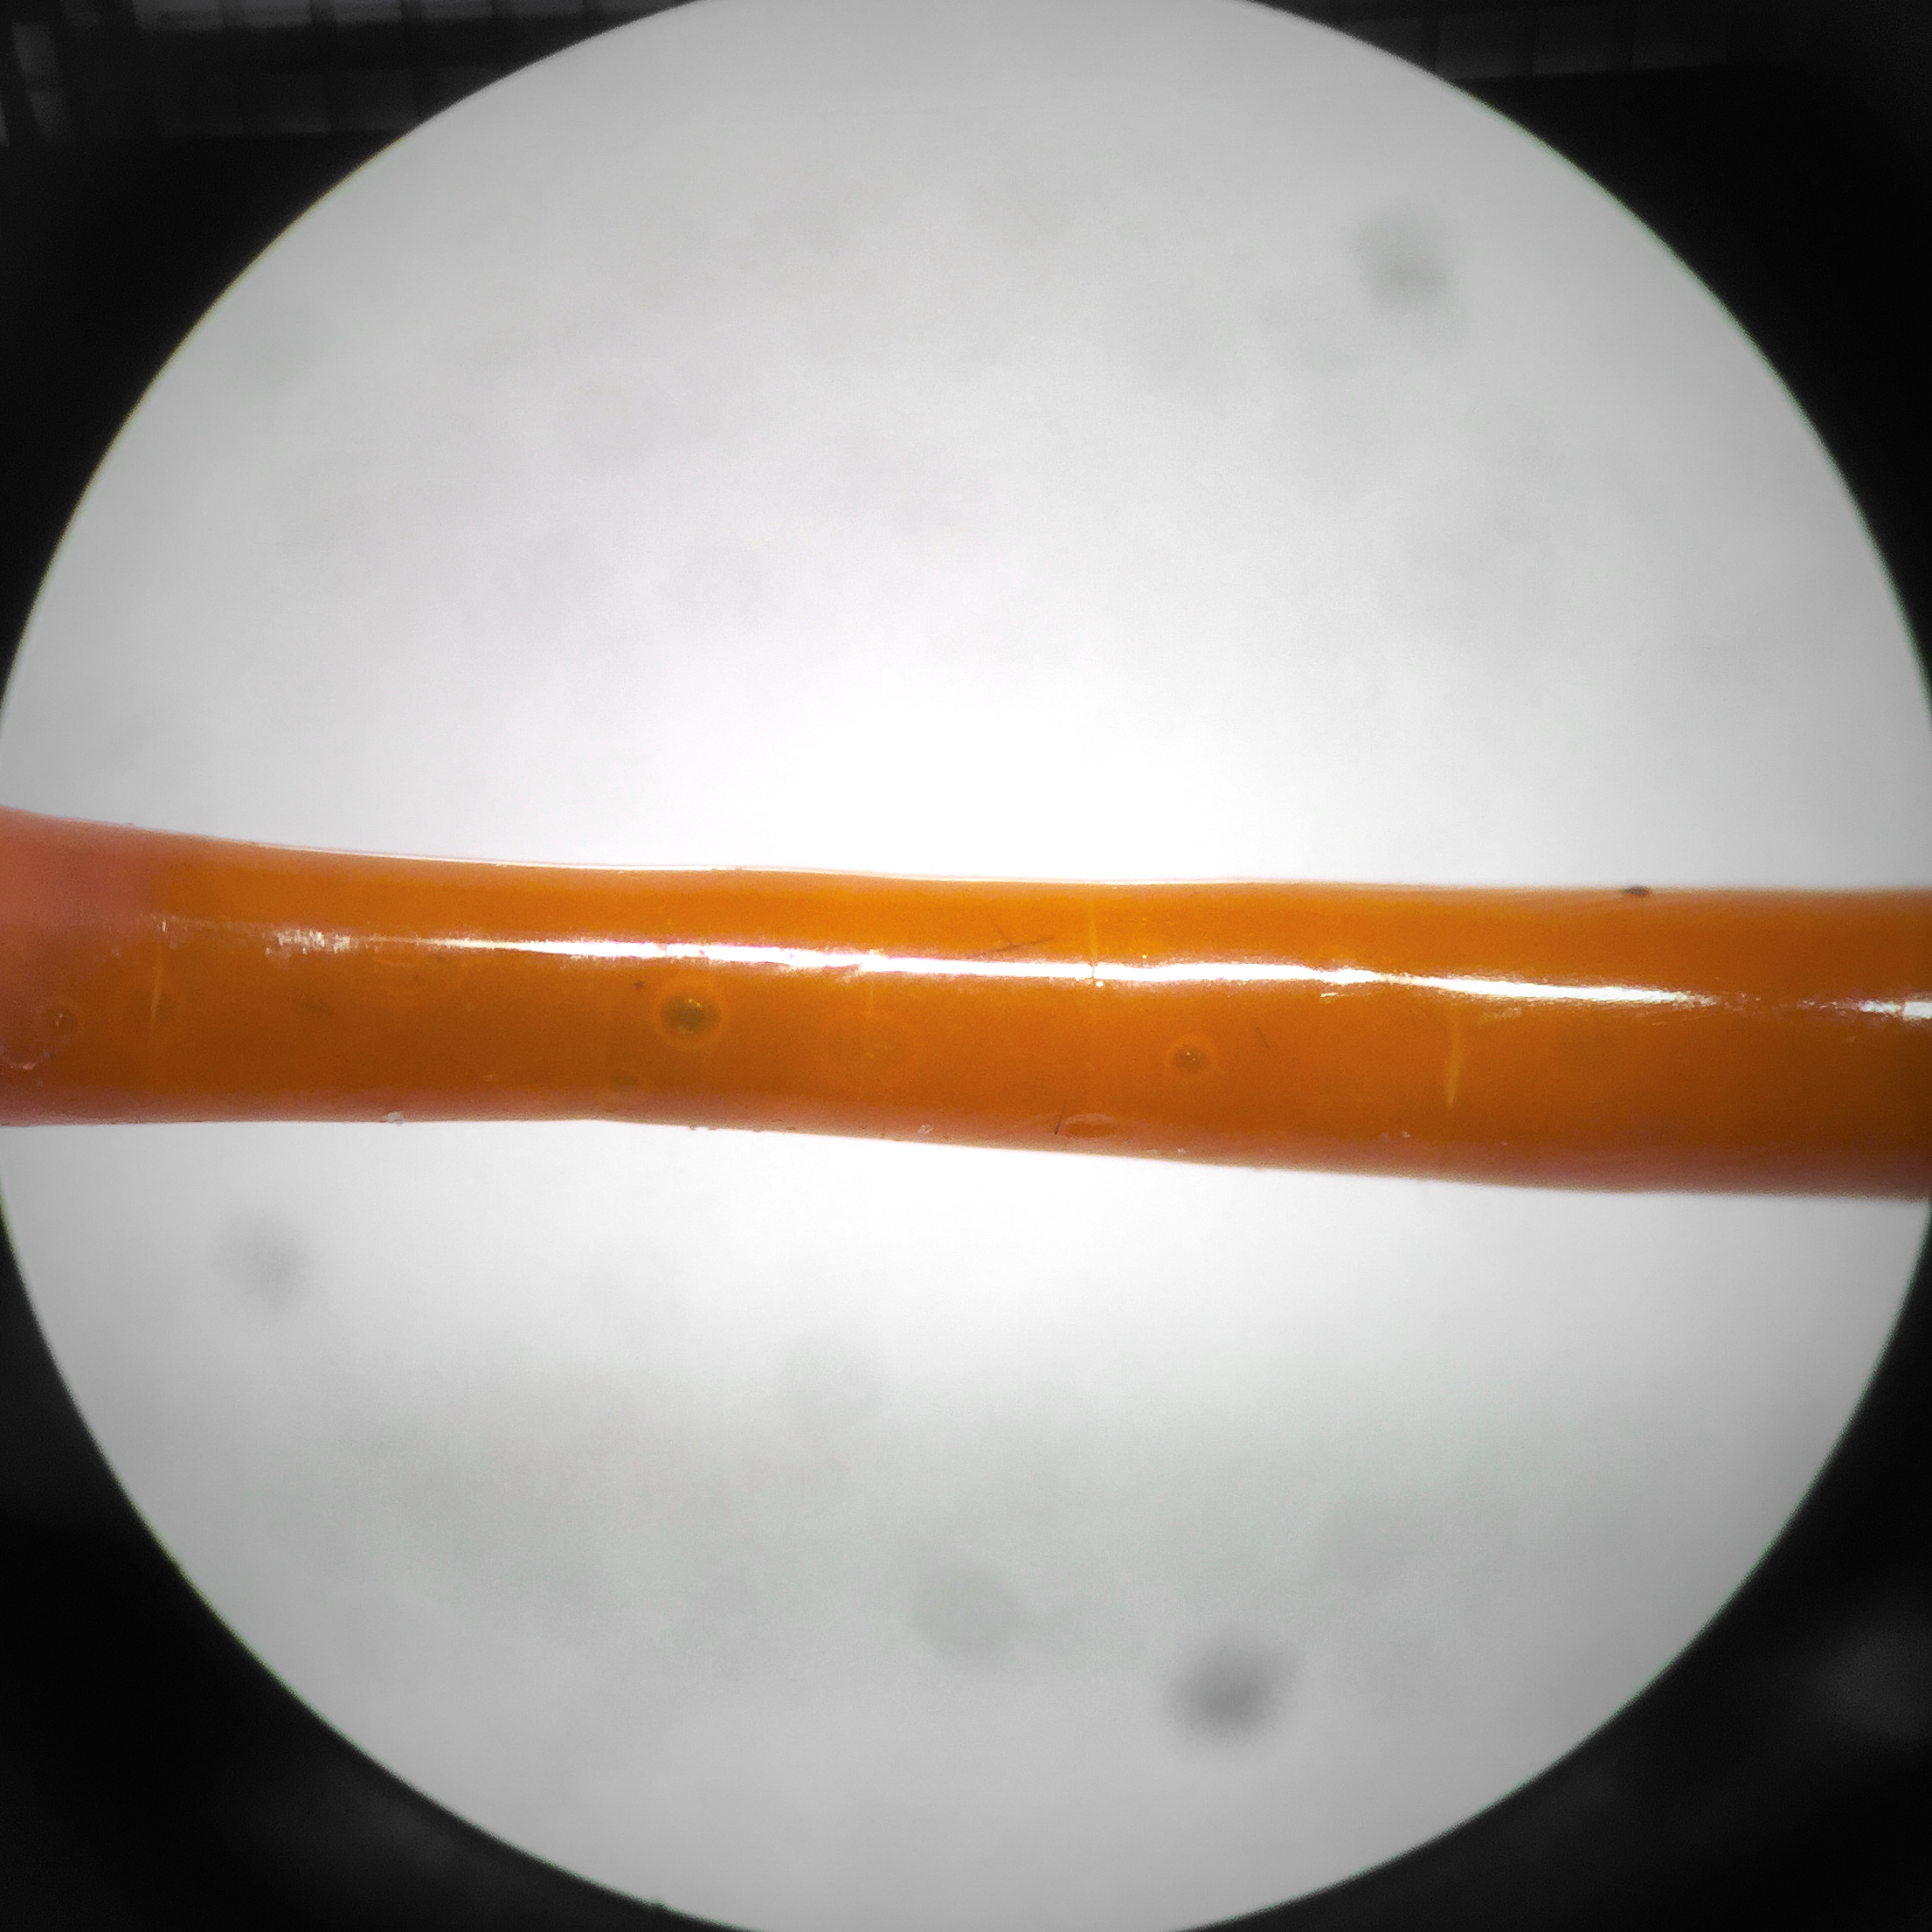
\includegraphics[width=\textwidth]{./figures/20-og-normal}
                \caption{Length normal.}
                \label{fig:20-og-normal}
        \end{subfigure}%
        ~ %add desired spacing between images, e. g. ~, \quad, \qquad, \hfill etc.
          %(or a blank line to force the subfigure onto a new line)
        \begin{subfigure}[b]{0.3\textwidth}
                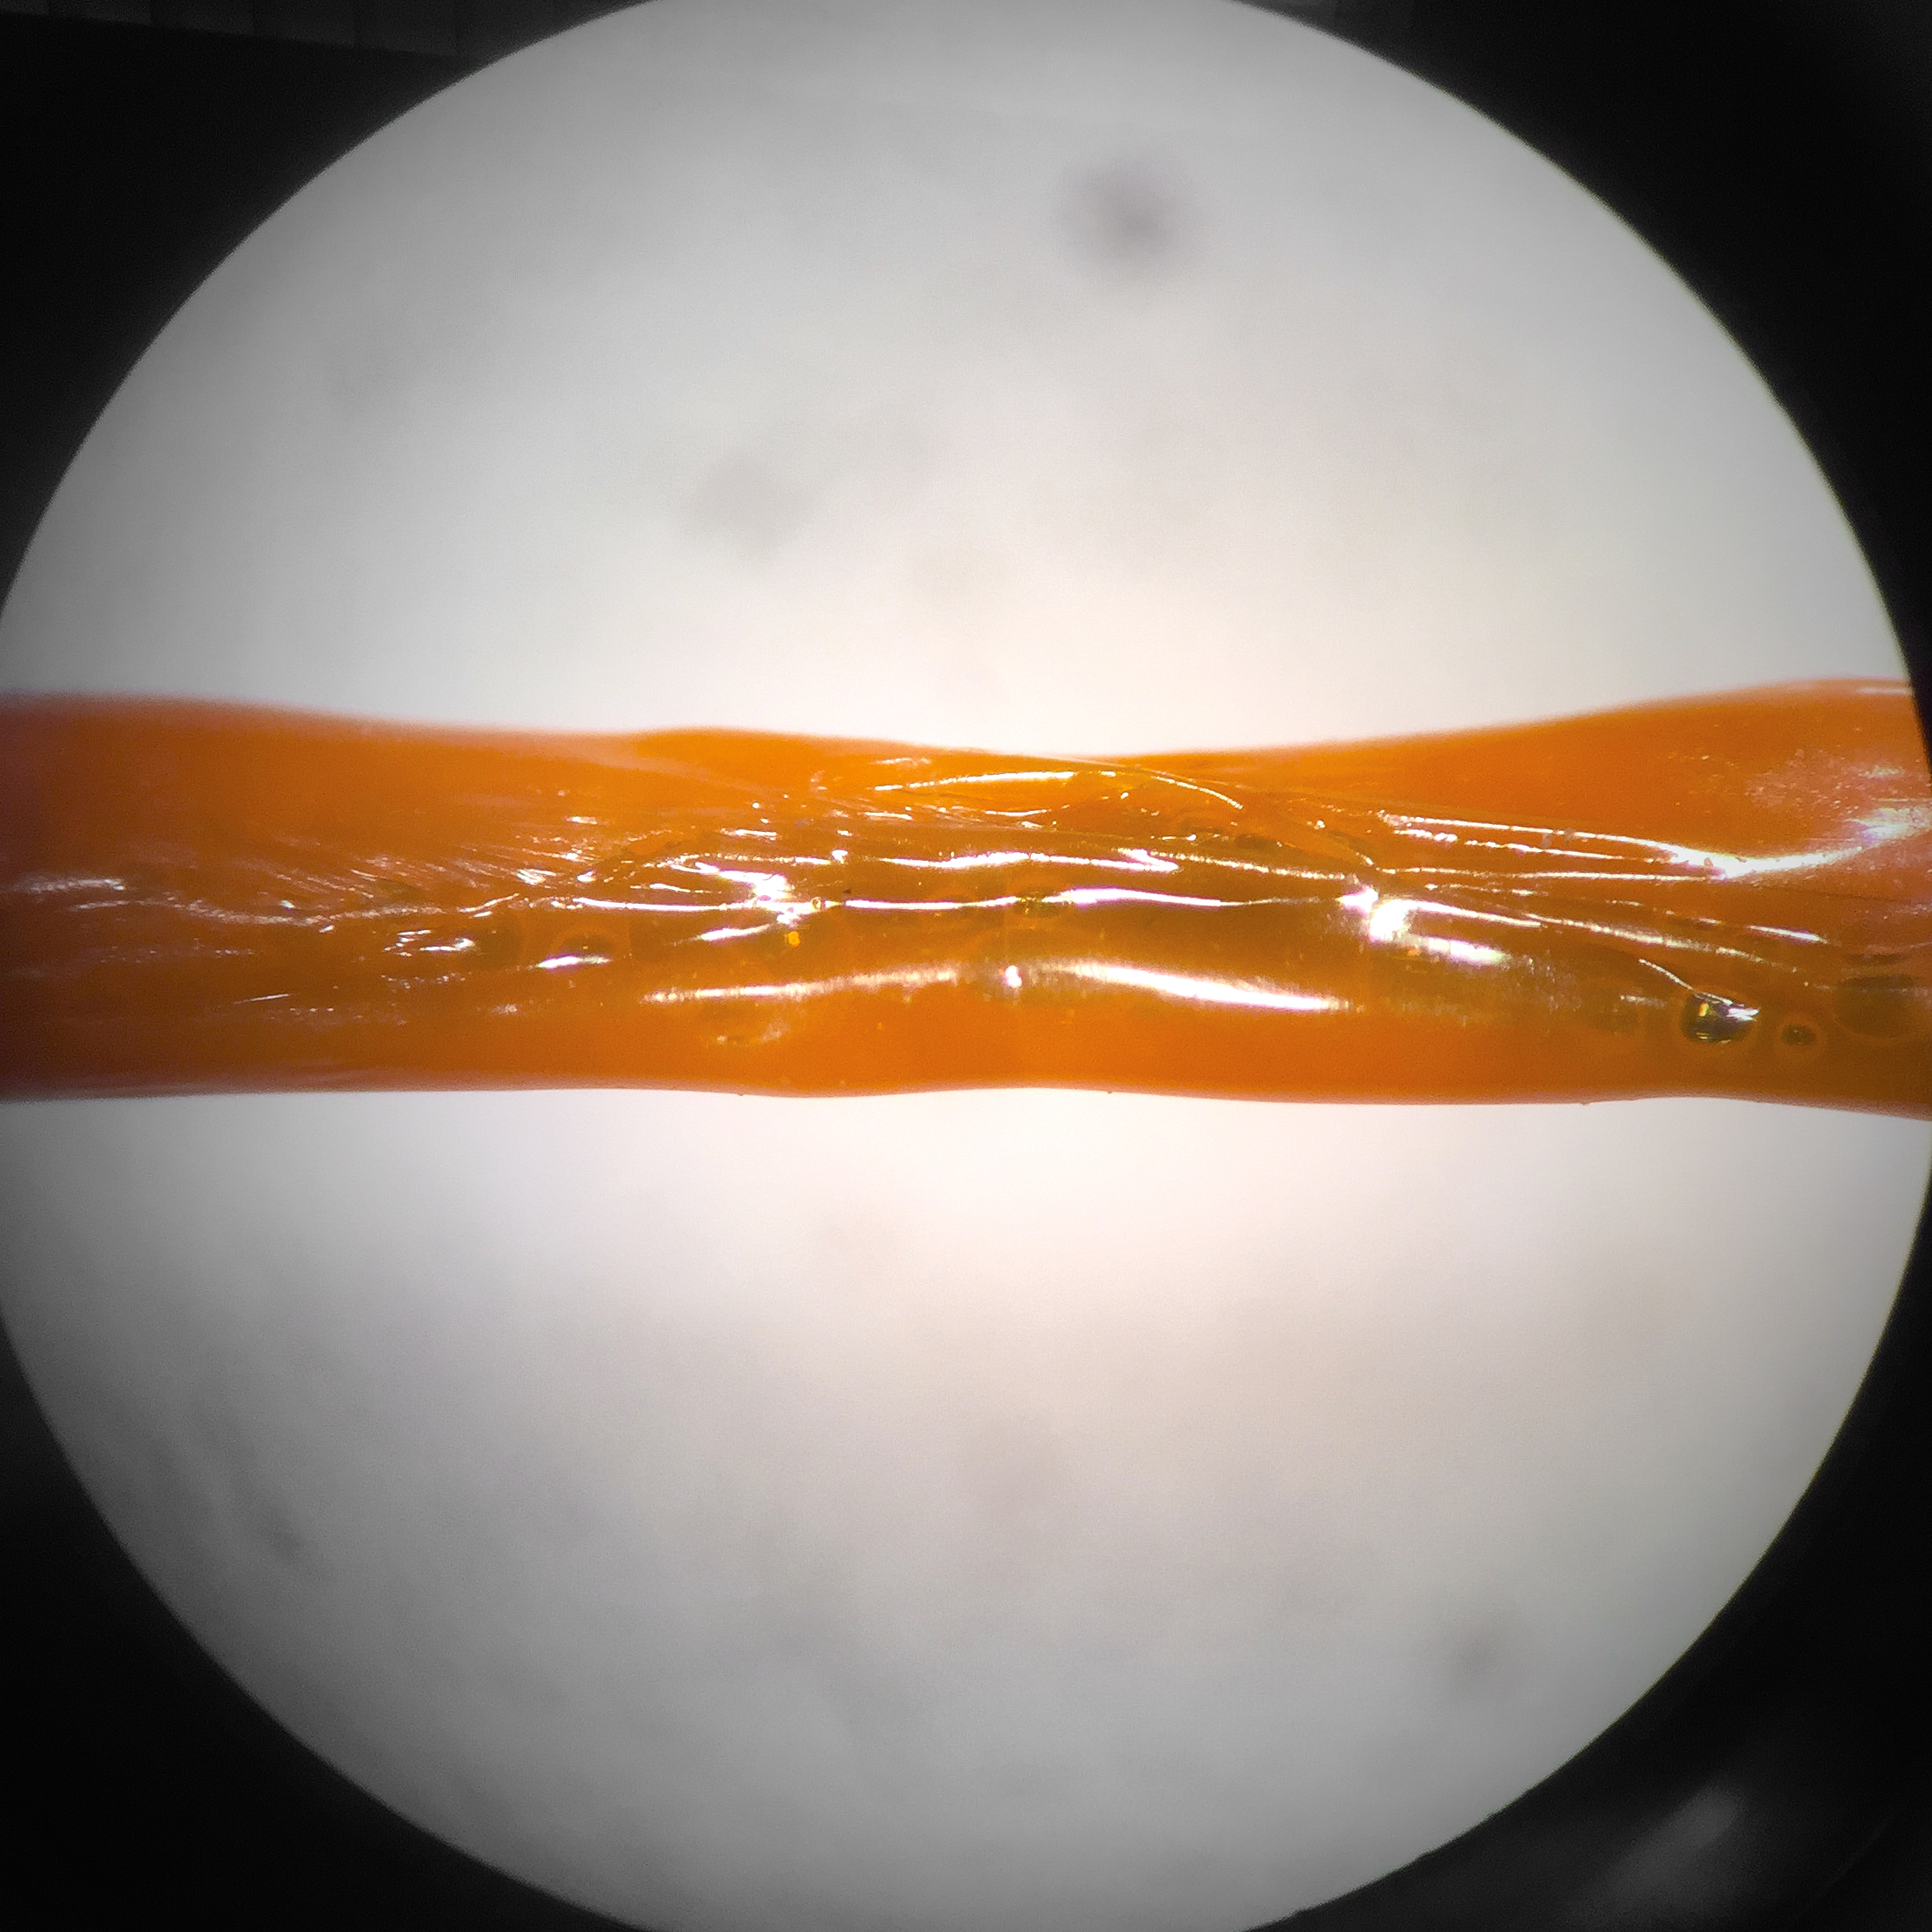
\includegraphics[width=\textwidth]{./figures/20-og-defect}
                \caption{Length defect.}
                \label{fig:20-og-defect}
        \end{subfigure}
        ~ %add desired spacing between images, e. g. ~, \quad, \qquad, \hfill etc.
          %(or a blank line to force the subfigure onto a new line)
        \begin{subfigure}[b]{0.3\textwidth}
                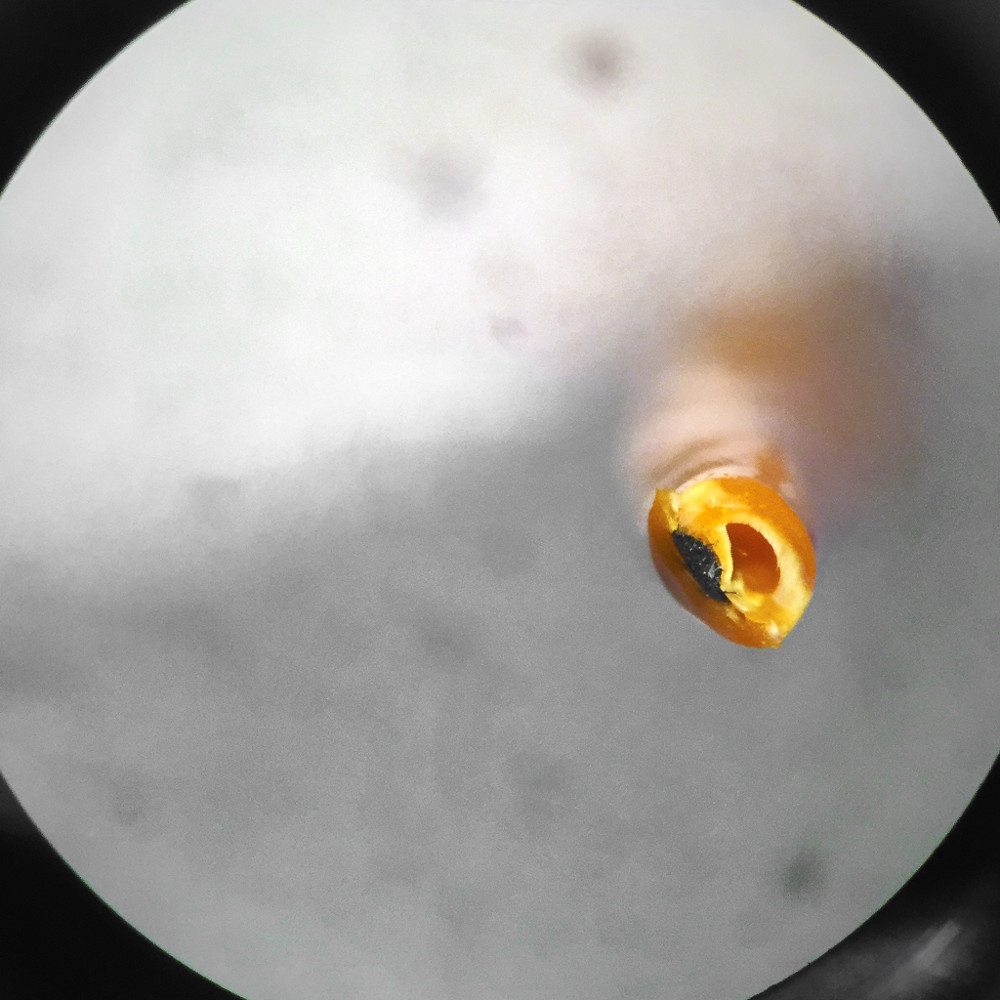
\includegraphics[width=\textwidth]{./figures/20-og-end}
                \caption{Cross section.}
                \label{fig:20-og-end}
        \end{subfigure}
        \caption{Microscopic views (10x) of a CFRP filament created with 20 dips using the partially immersed guide.}\label{fig:20-og}
\end{figure}

% inernal guide

\begin{figure}[h!]
        \centering
        \begin{subfigure}[b]{0.3\textwidth}
                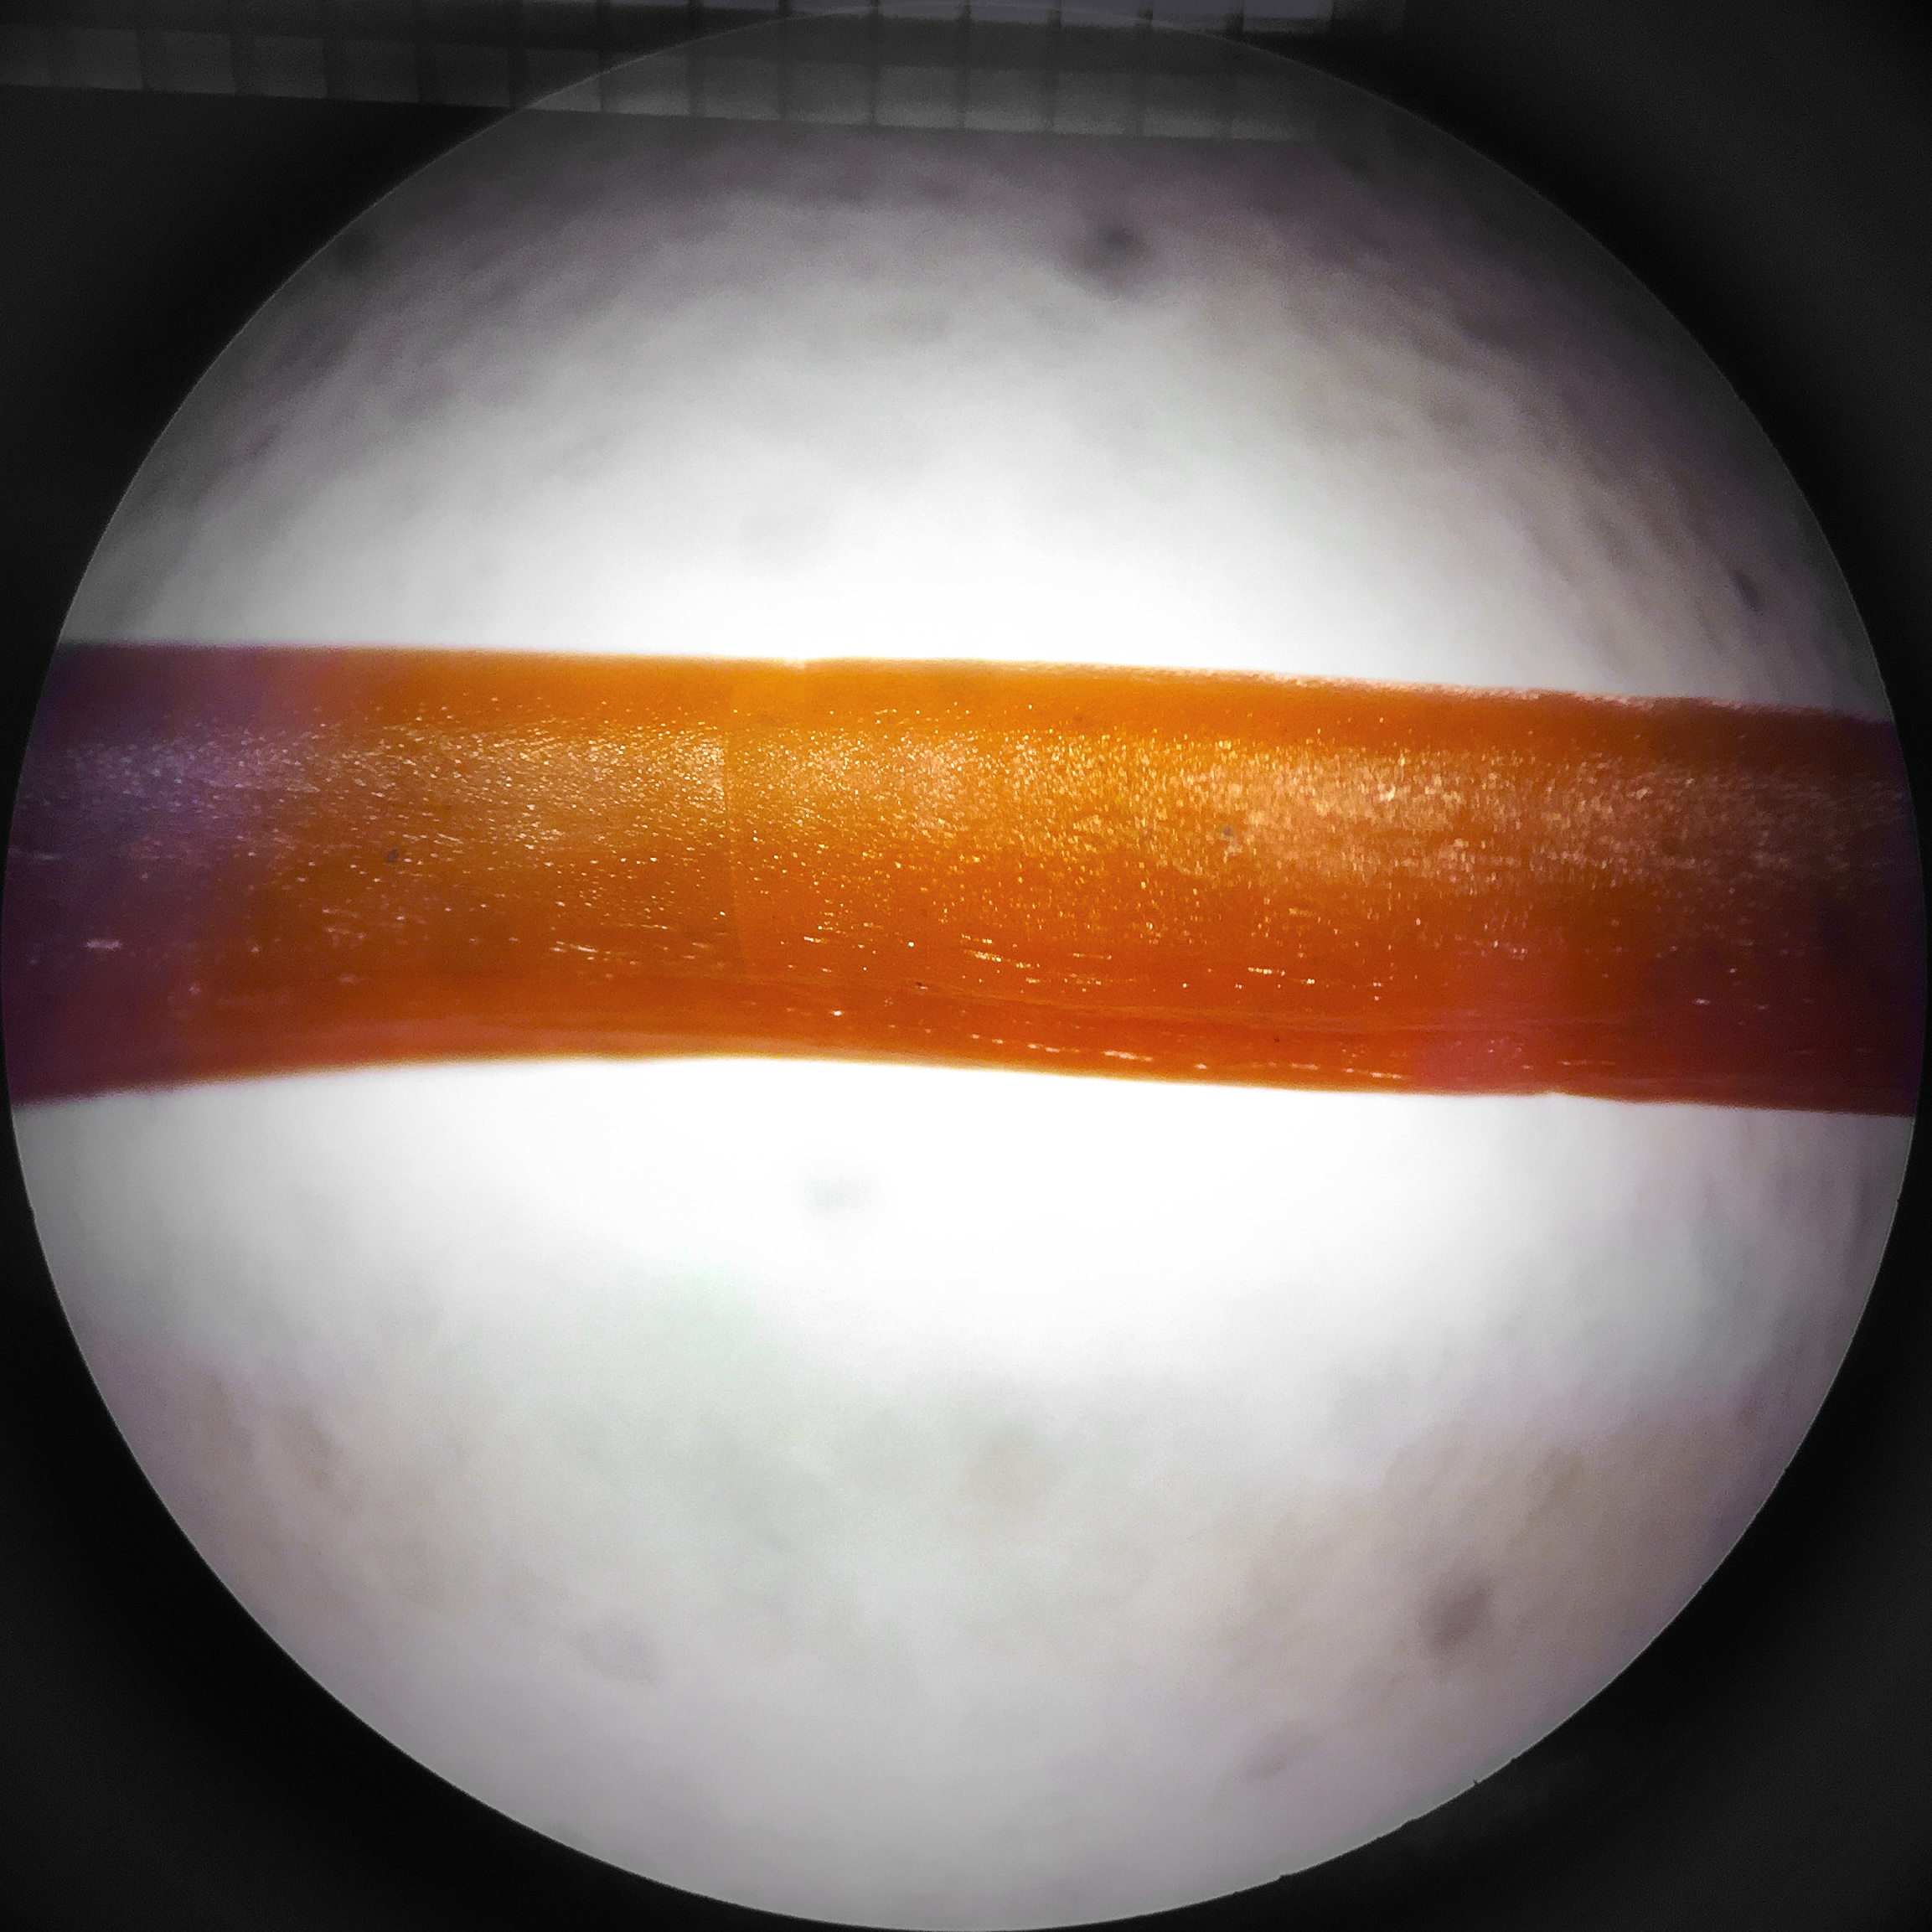
\includegraphics[width=\textwidth]{./figures/20-ng-normal}
                \caption{Length normal.}
                \label{fig:20-og-normal}
        \end{subfigure}%
        ~ %add desired spacing between images, e. g. ~, \quad, \qquad, \hfill etc.
          %(or a blank line to force the subfigure onto a new line)
        \begin{subfigure}[b]{0.3\textwidth}
                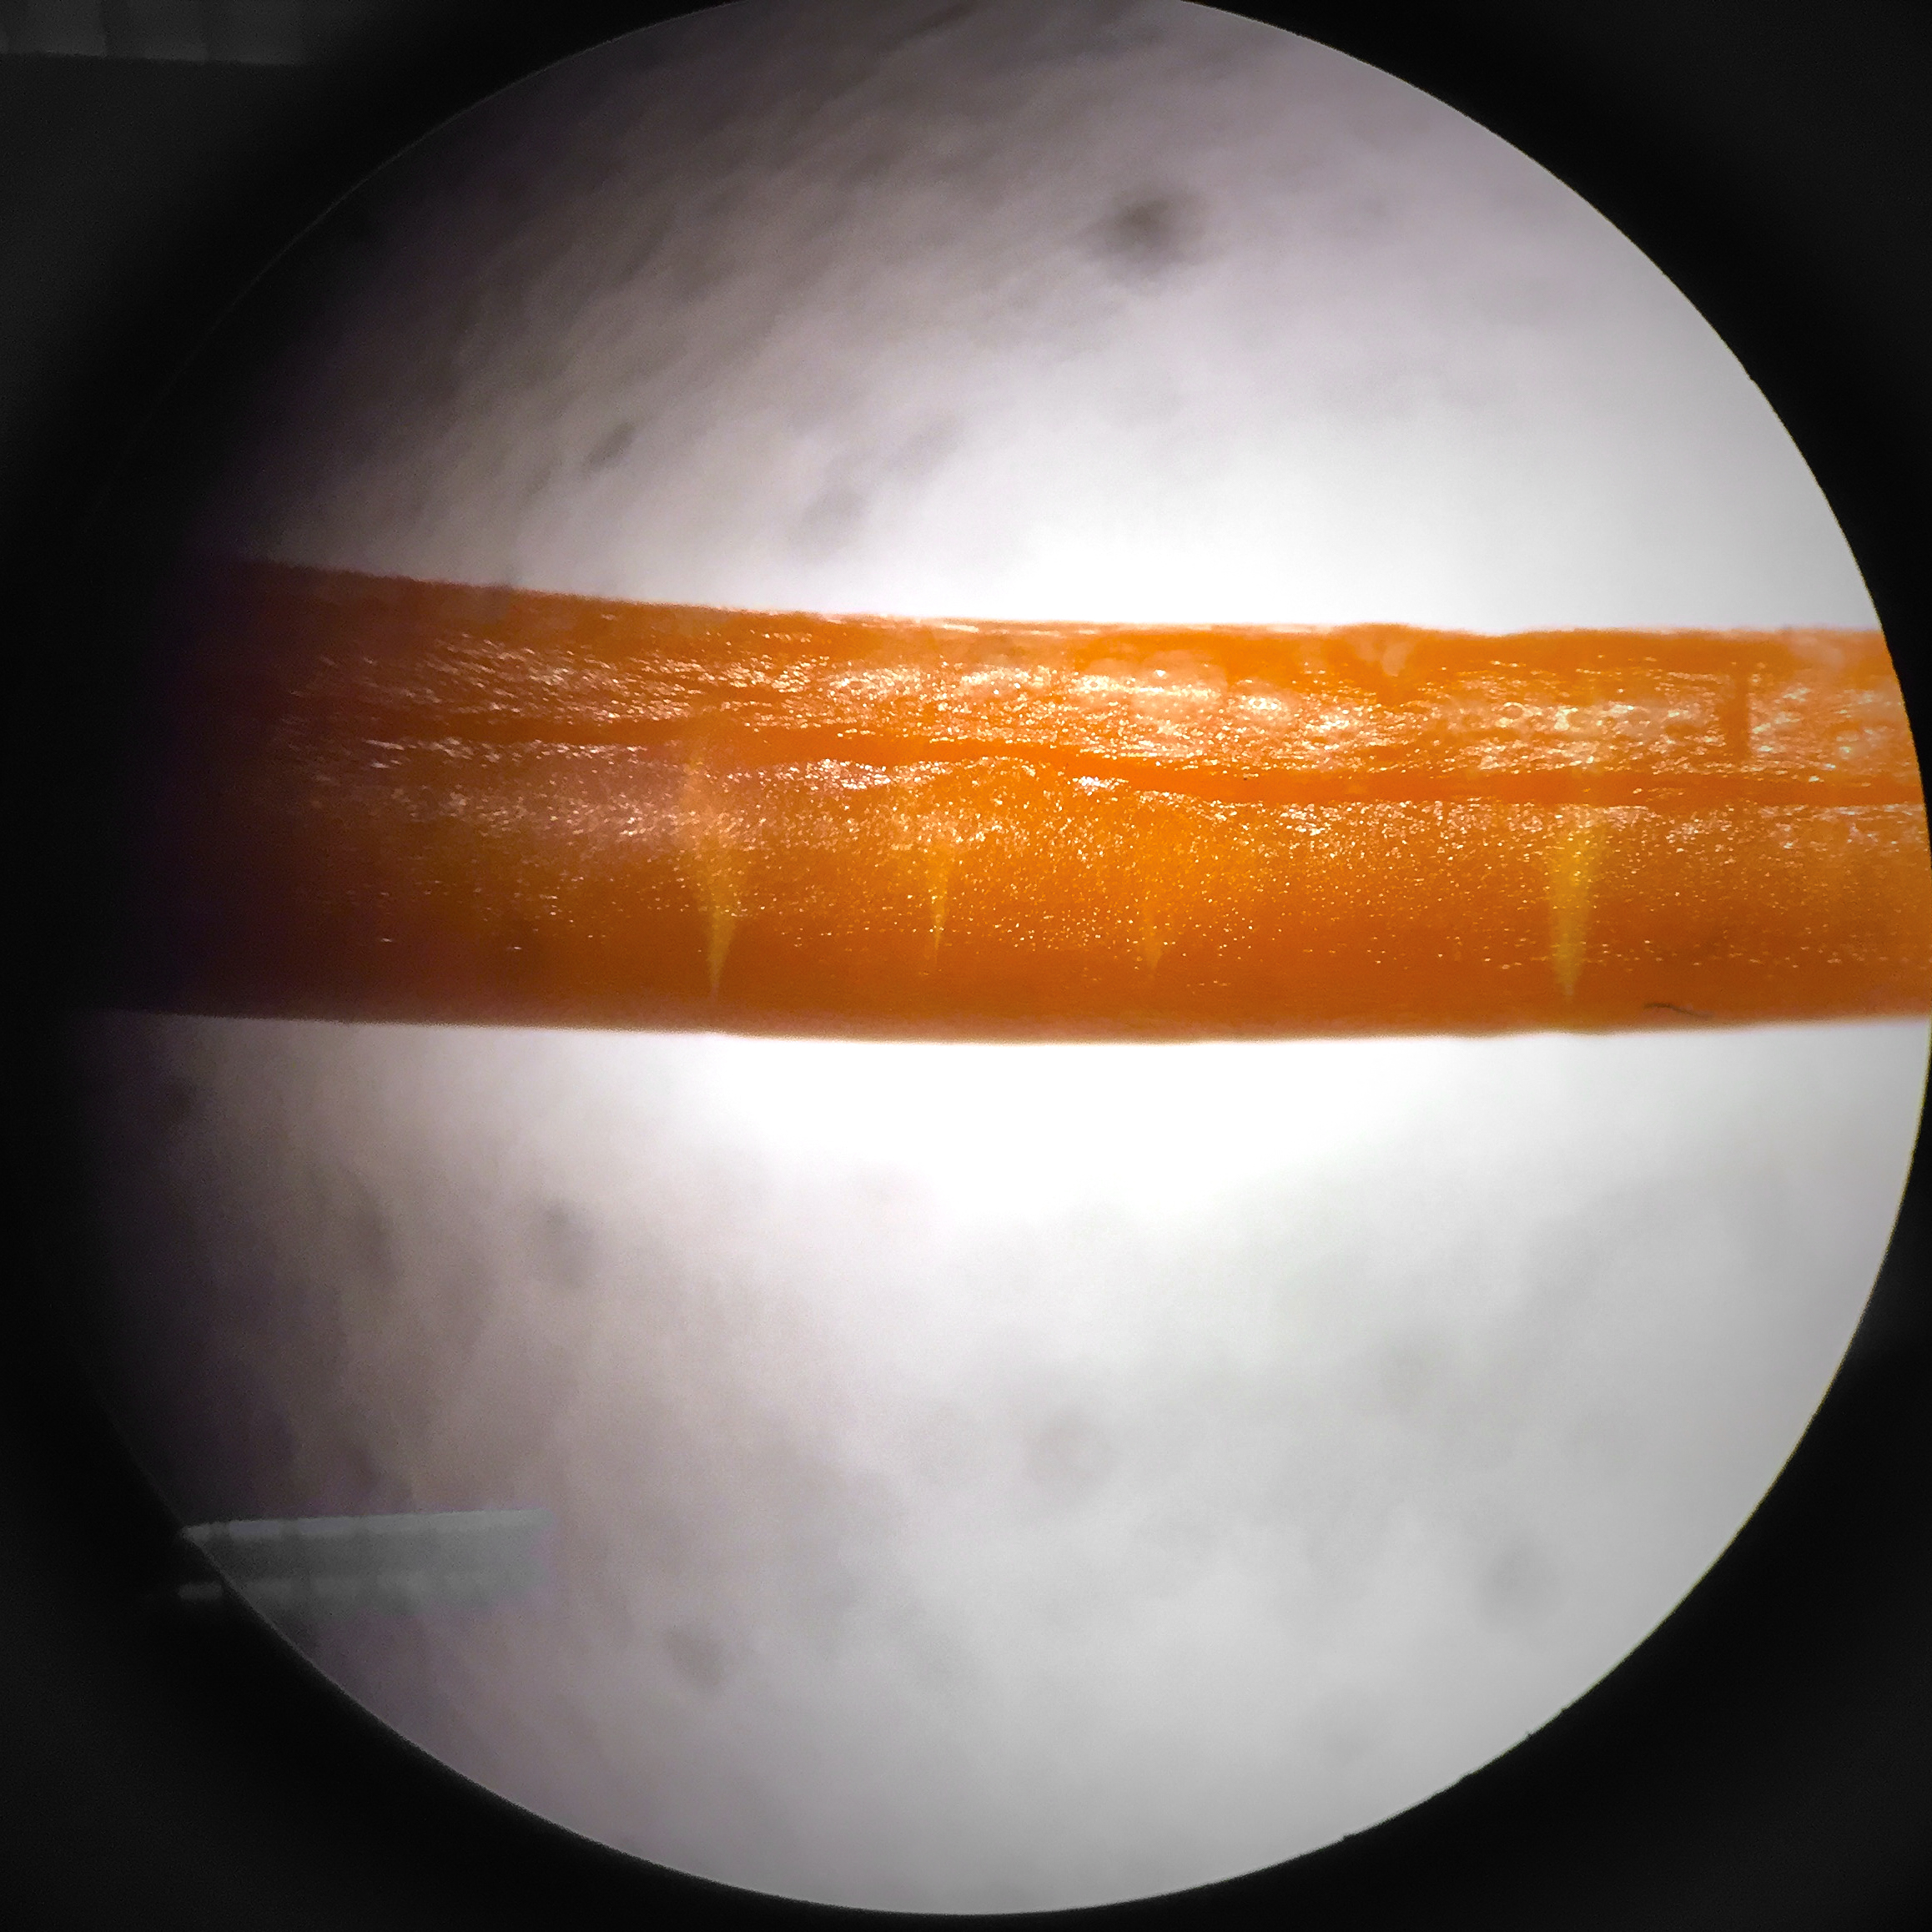
\includegraphics[width=\textwidth]{./figures/20-ng-defect}
                \caption{Length defect.}
                \label{fig:20-og-defect}
        \end{subfigure}
        ~ %add desired spacing between images, e. g. ~, \quad, \qquad, \hfill etc.
          %(or a blank line to force the subfigure onto a new line)
        \begin{subfigure}[b]{0.3\textwidth}
                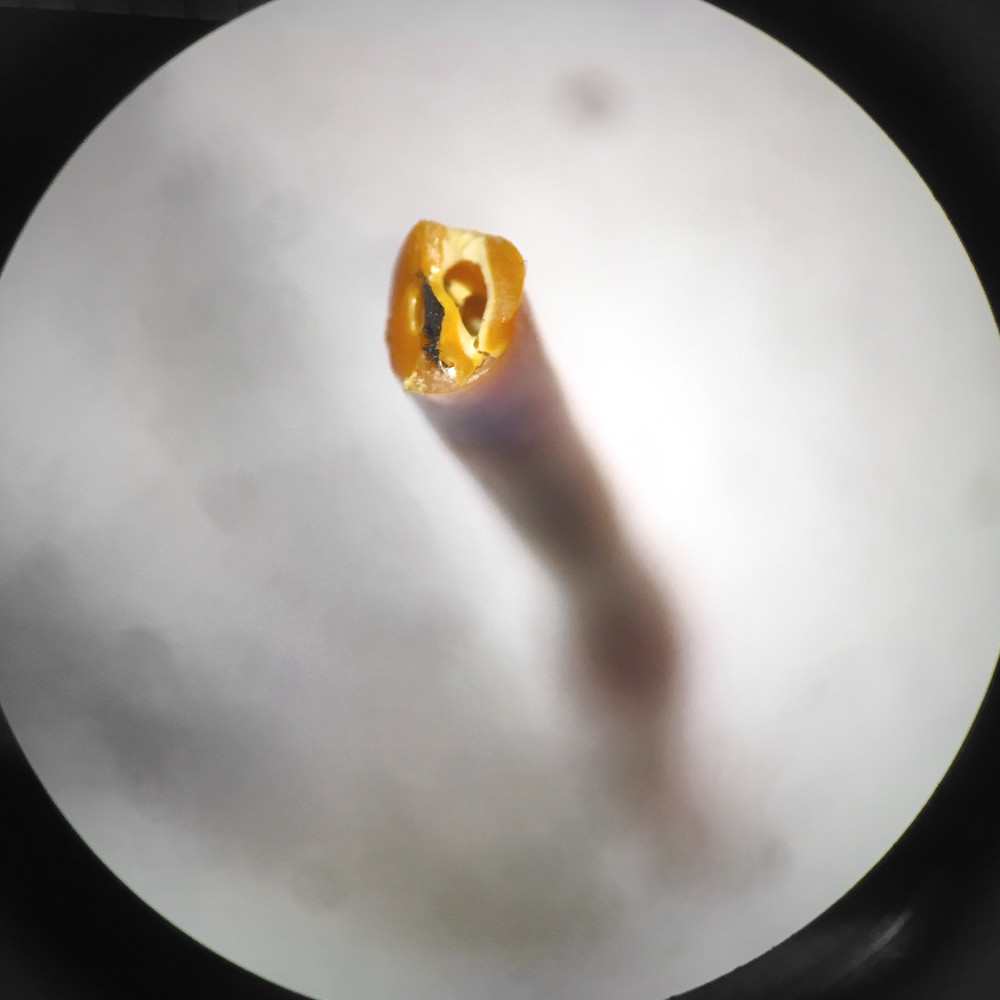
\includegraphics[width=\textwidth]{./figures/20-ng-end}
                \caption{Cross section.}
                \label{fig:20-og-end}
        \end{subfigure}
        \caption{Microscopic views (10x) of a CFRP filament created with 20 dips using the fully immersed guide.}\label{fig:20-ng}
\end{figure}

% 108 40 dip

\begin{figure}[h!]
        \centering
        \begin{subfigure}[b]{0.3\textwidth}
                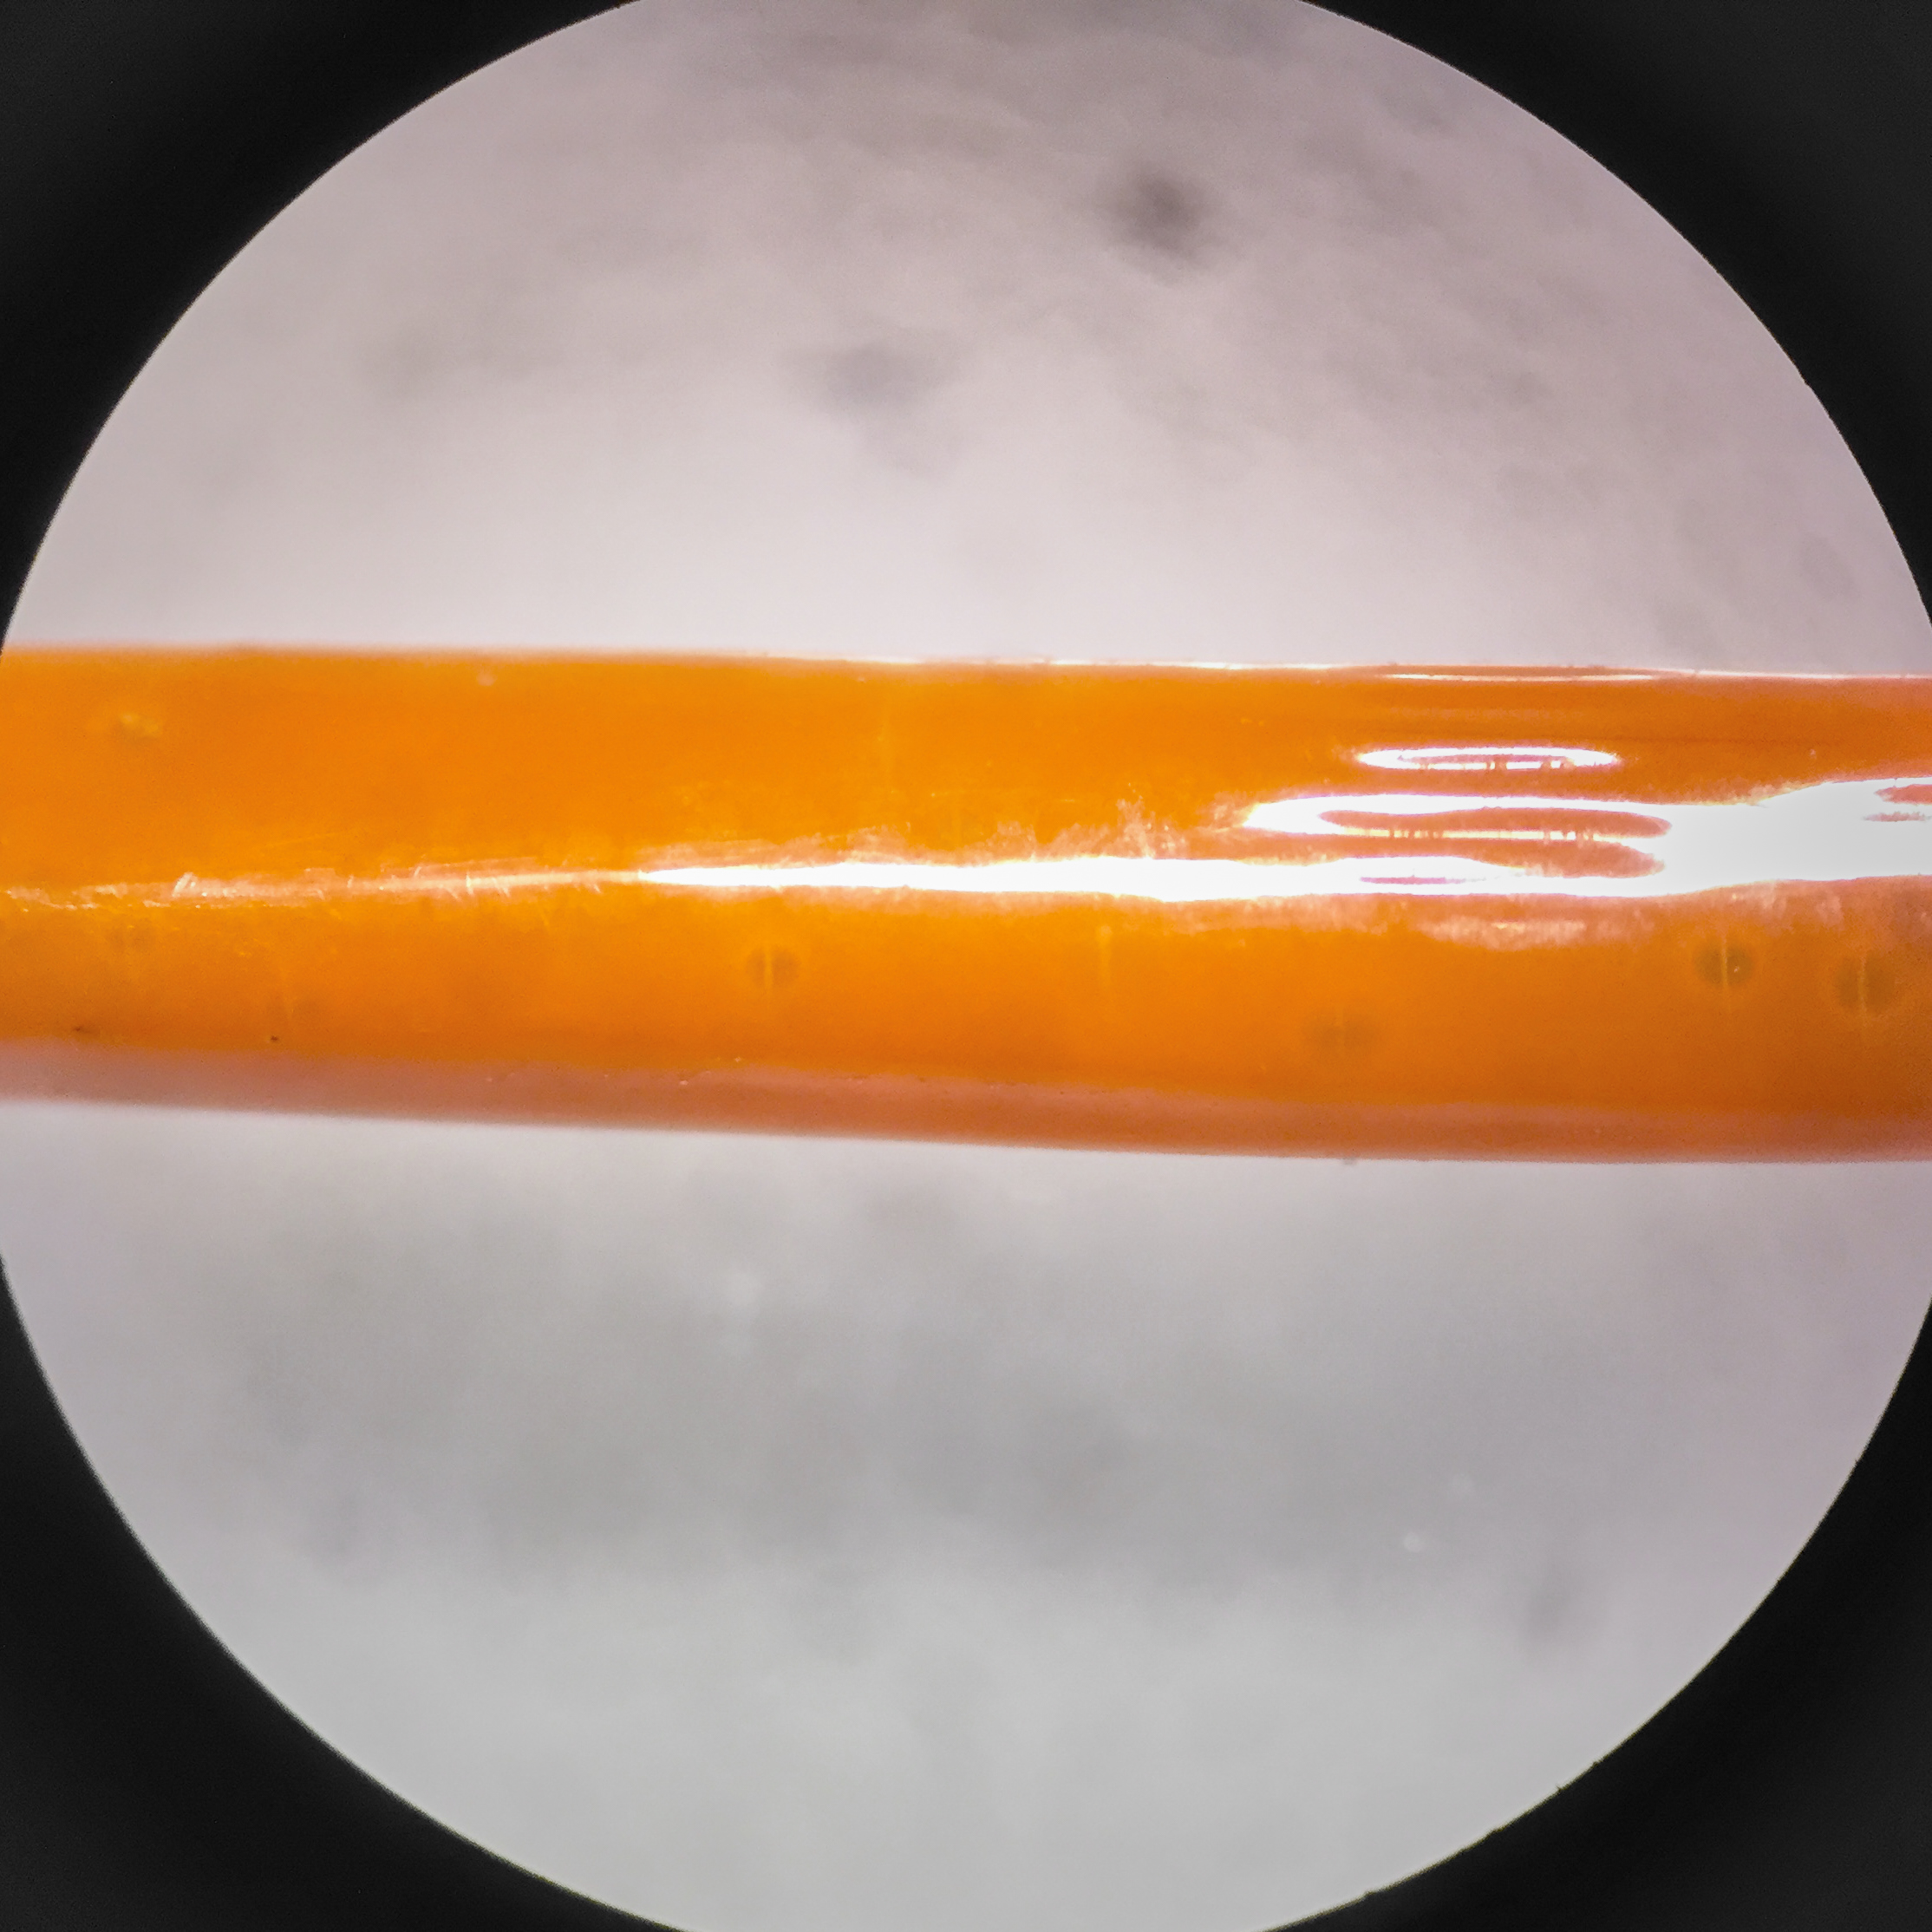
\includegraphics[width=\textwidth]{./figures/filament-108-40-dip-side}
                \caption{Length.}
                \label{fig:filament-108-40-dip-side}
        \end{subfigure}
        \begin{subfigure}[b]{0.3\textwidth}
                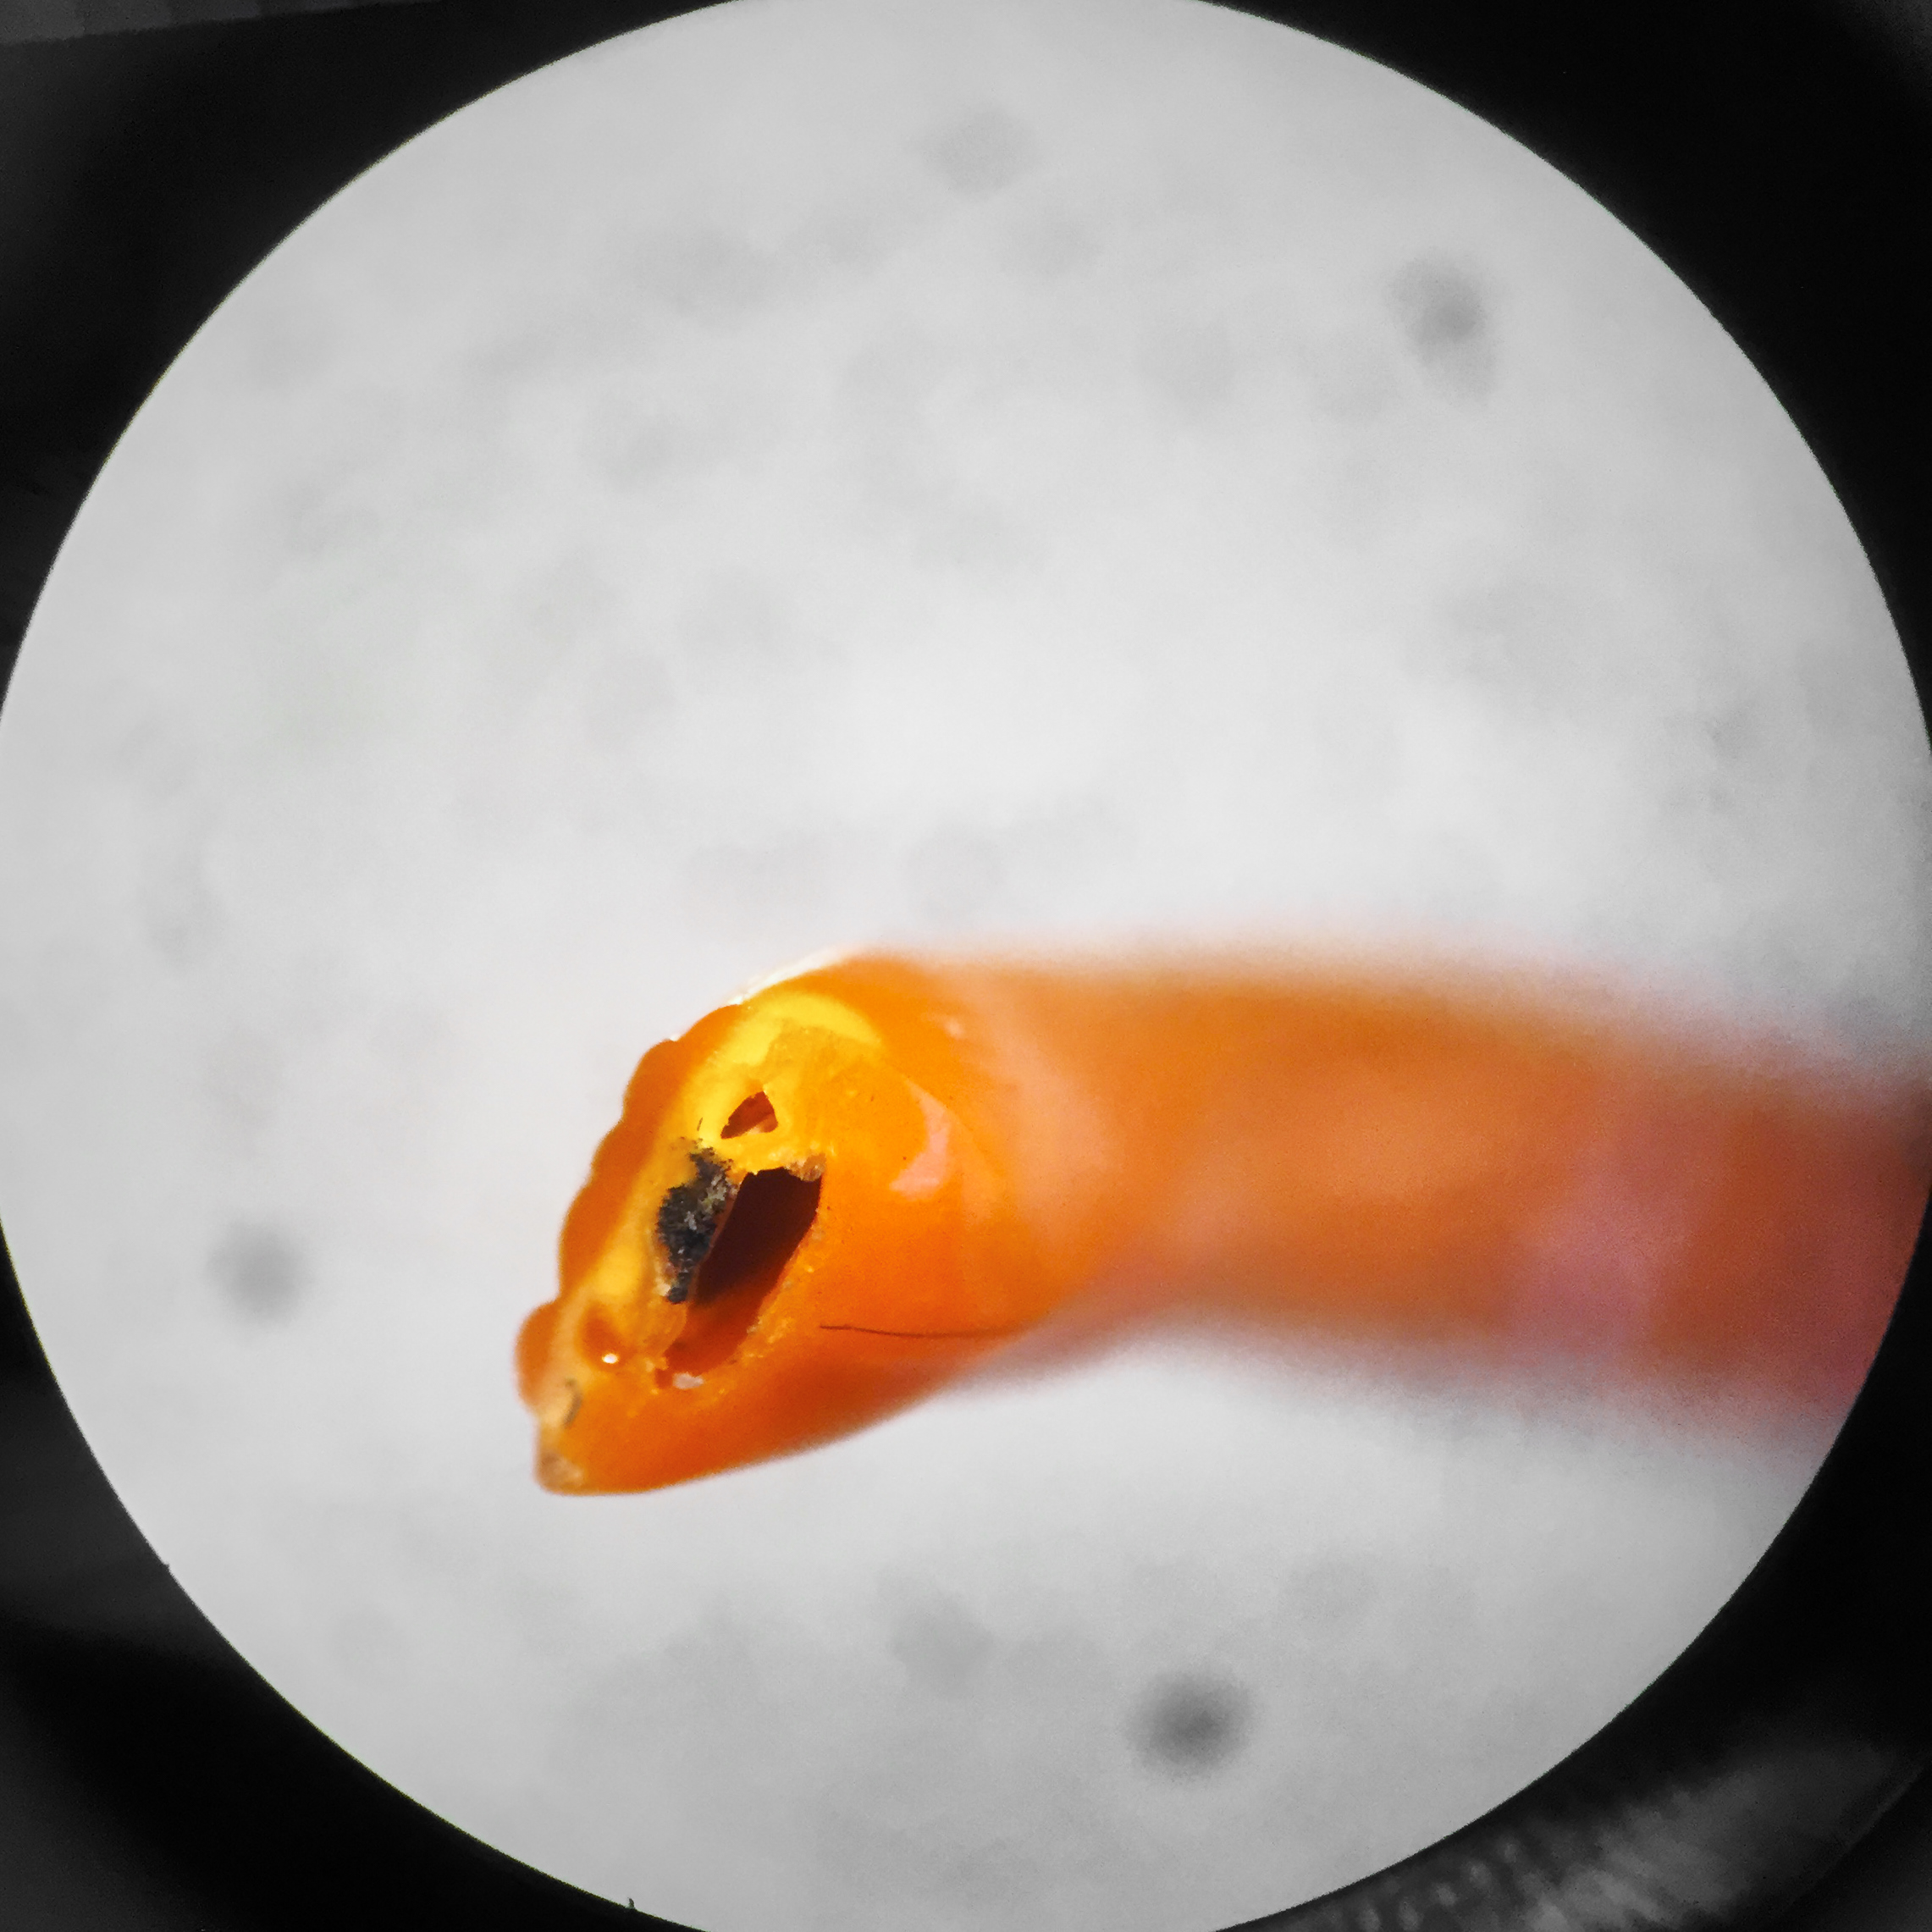
\includegraphics[width=\textwidth]{./figures/filament-108-40-dip-end}
                \caption{Cross section.}
                \label{fig:filament-108-40-dip-end}
        \end{subfigure}
        \caption{Microscopic views (10x) of a CFRP filament created with 10 dips using the fully immersed guide in a 4\% ABS solution.}\label{fig:filament-108-40-dip-microscope}
\end{figure}

% 108 40 bath

\begin{figure}[h!]
        \centering
        \begin{subfigure}[b]{0.3\textwidth}
                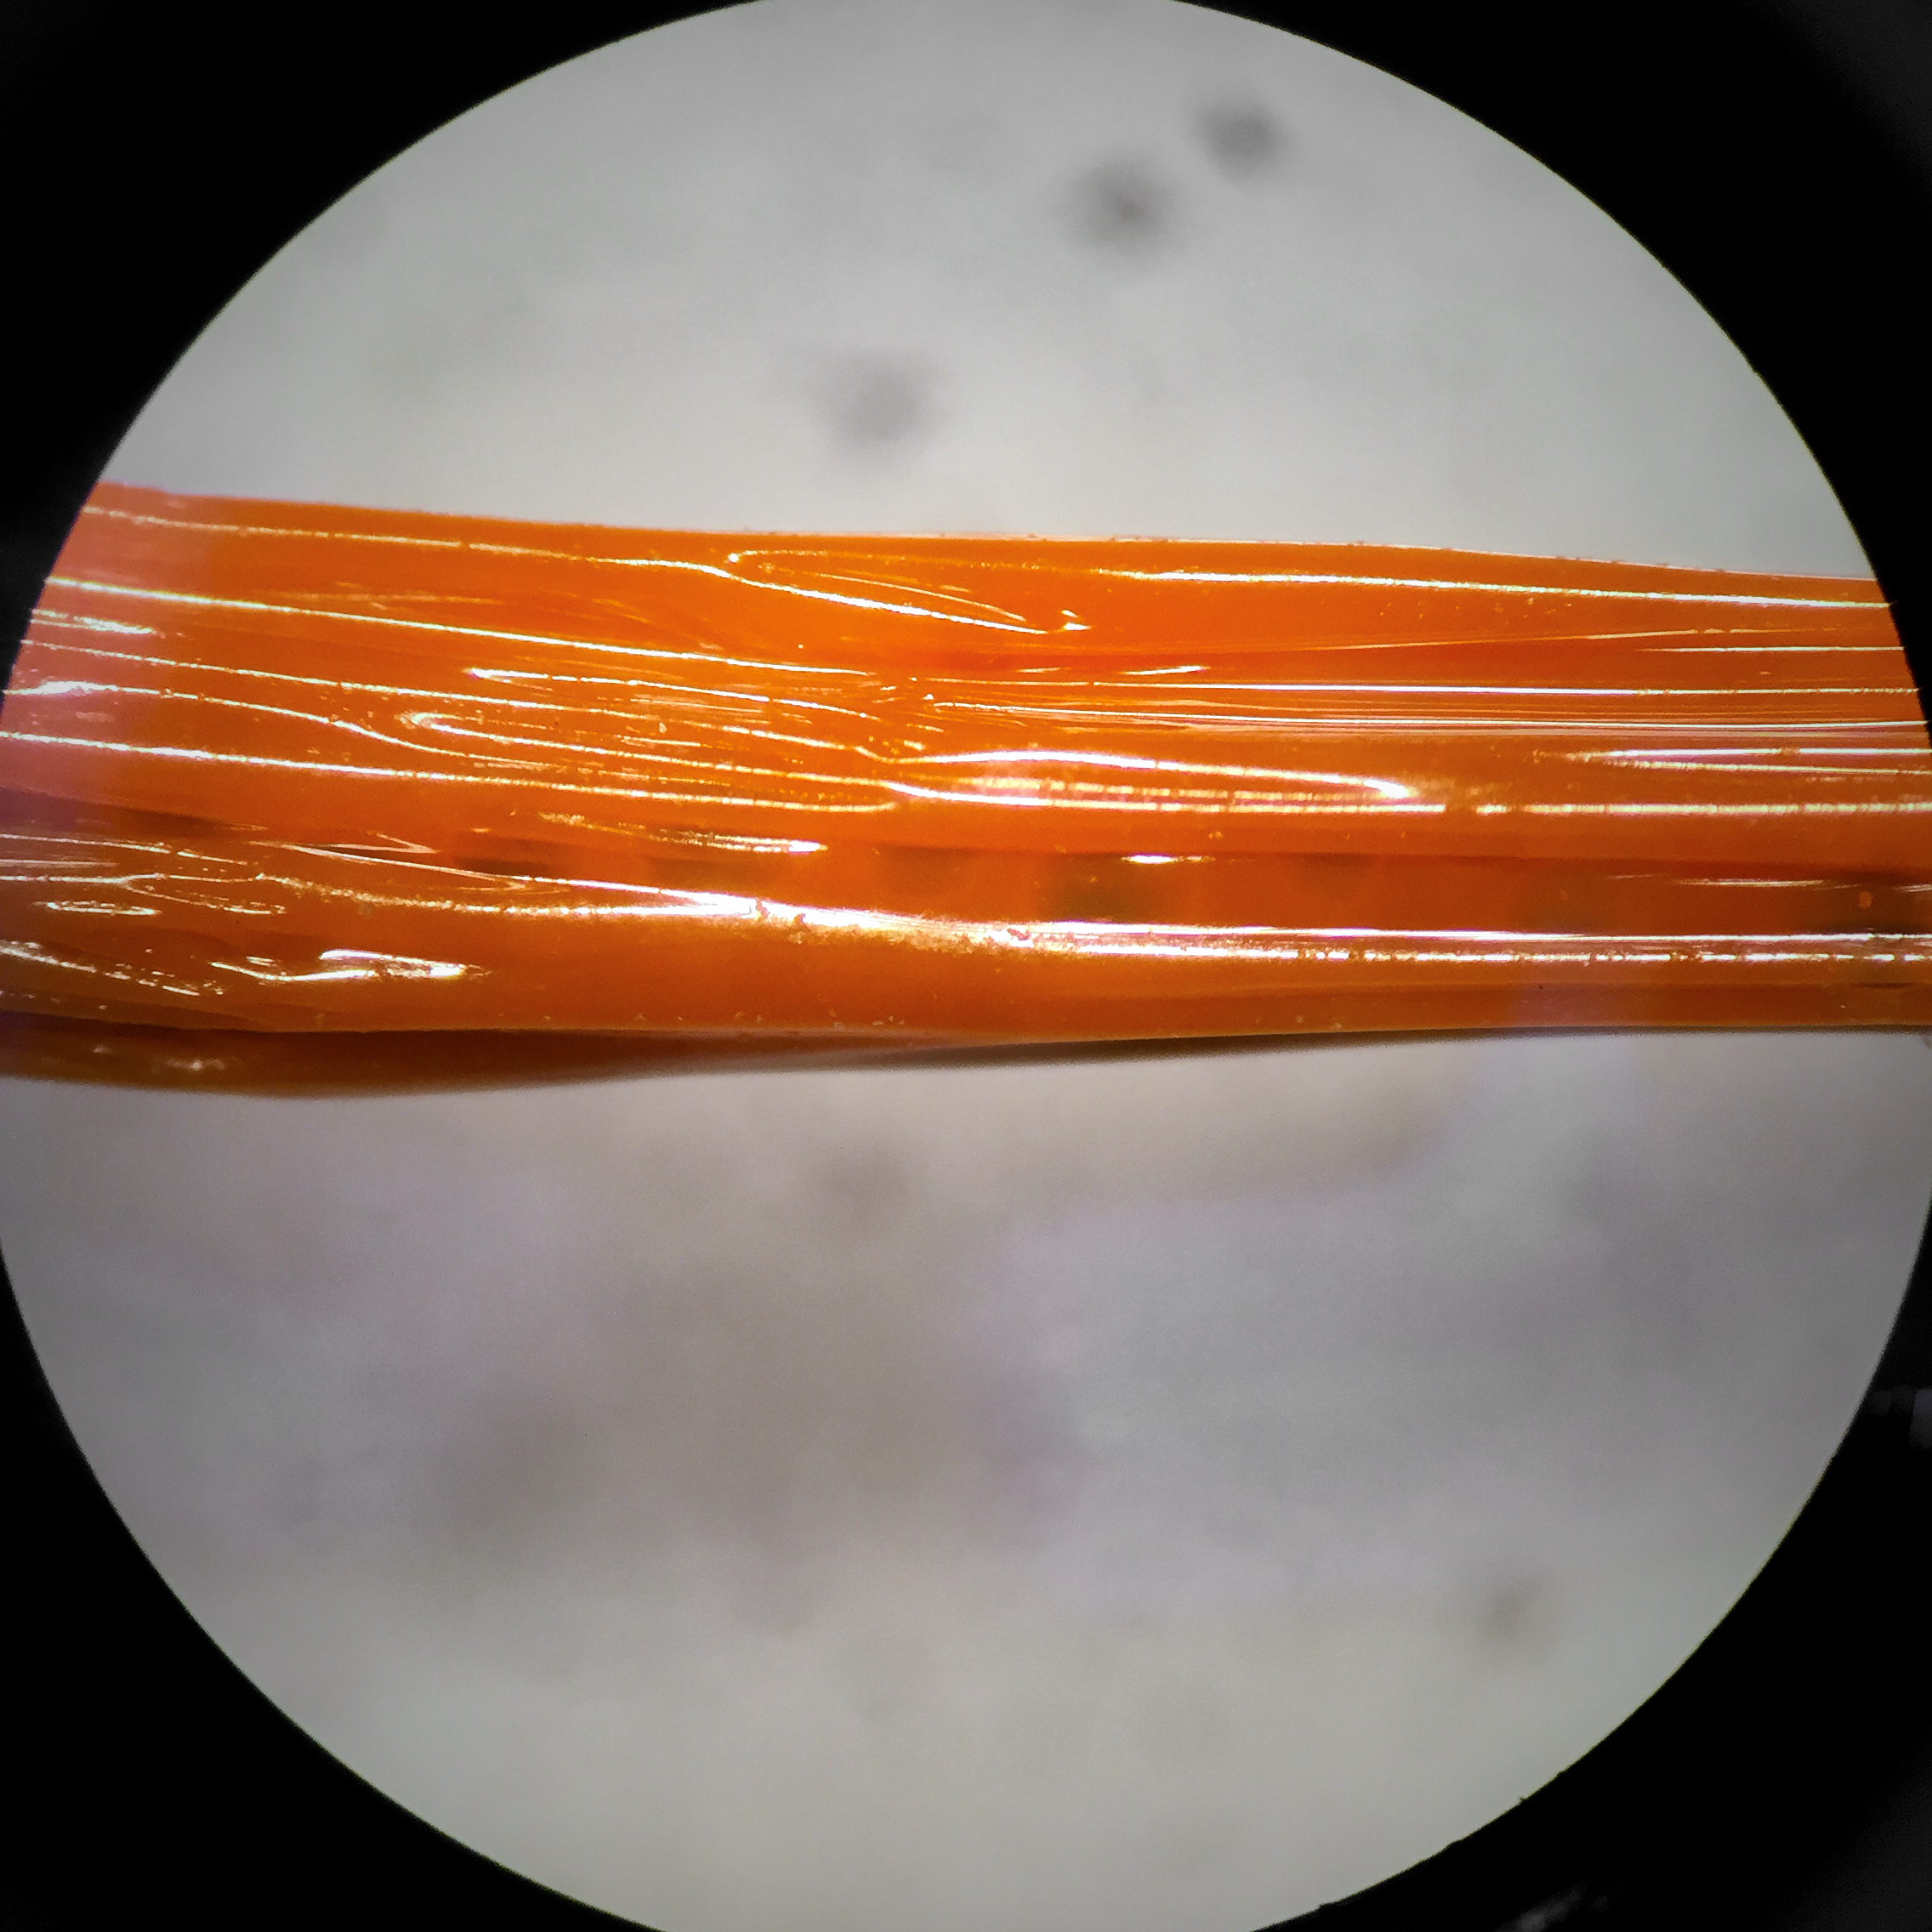
\includegraphics[width=\textwidth]{./figures/filament-108-40-flat-side}
                \caption{Length.}
                \label{fig:filament-108-40-flat-side}
        \end{subfigure}
        \begin{subfigure}[b]{0.3\textwidth}
                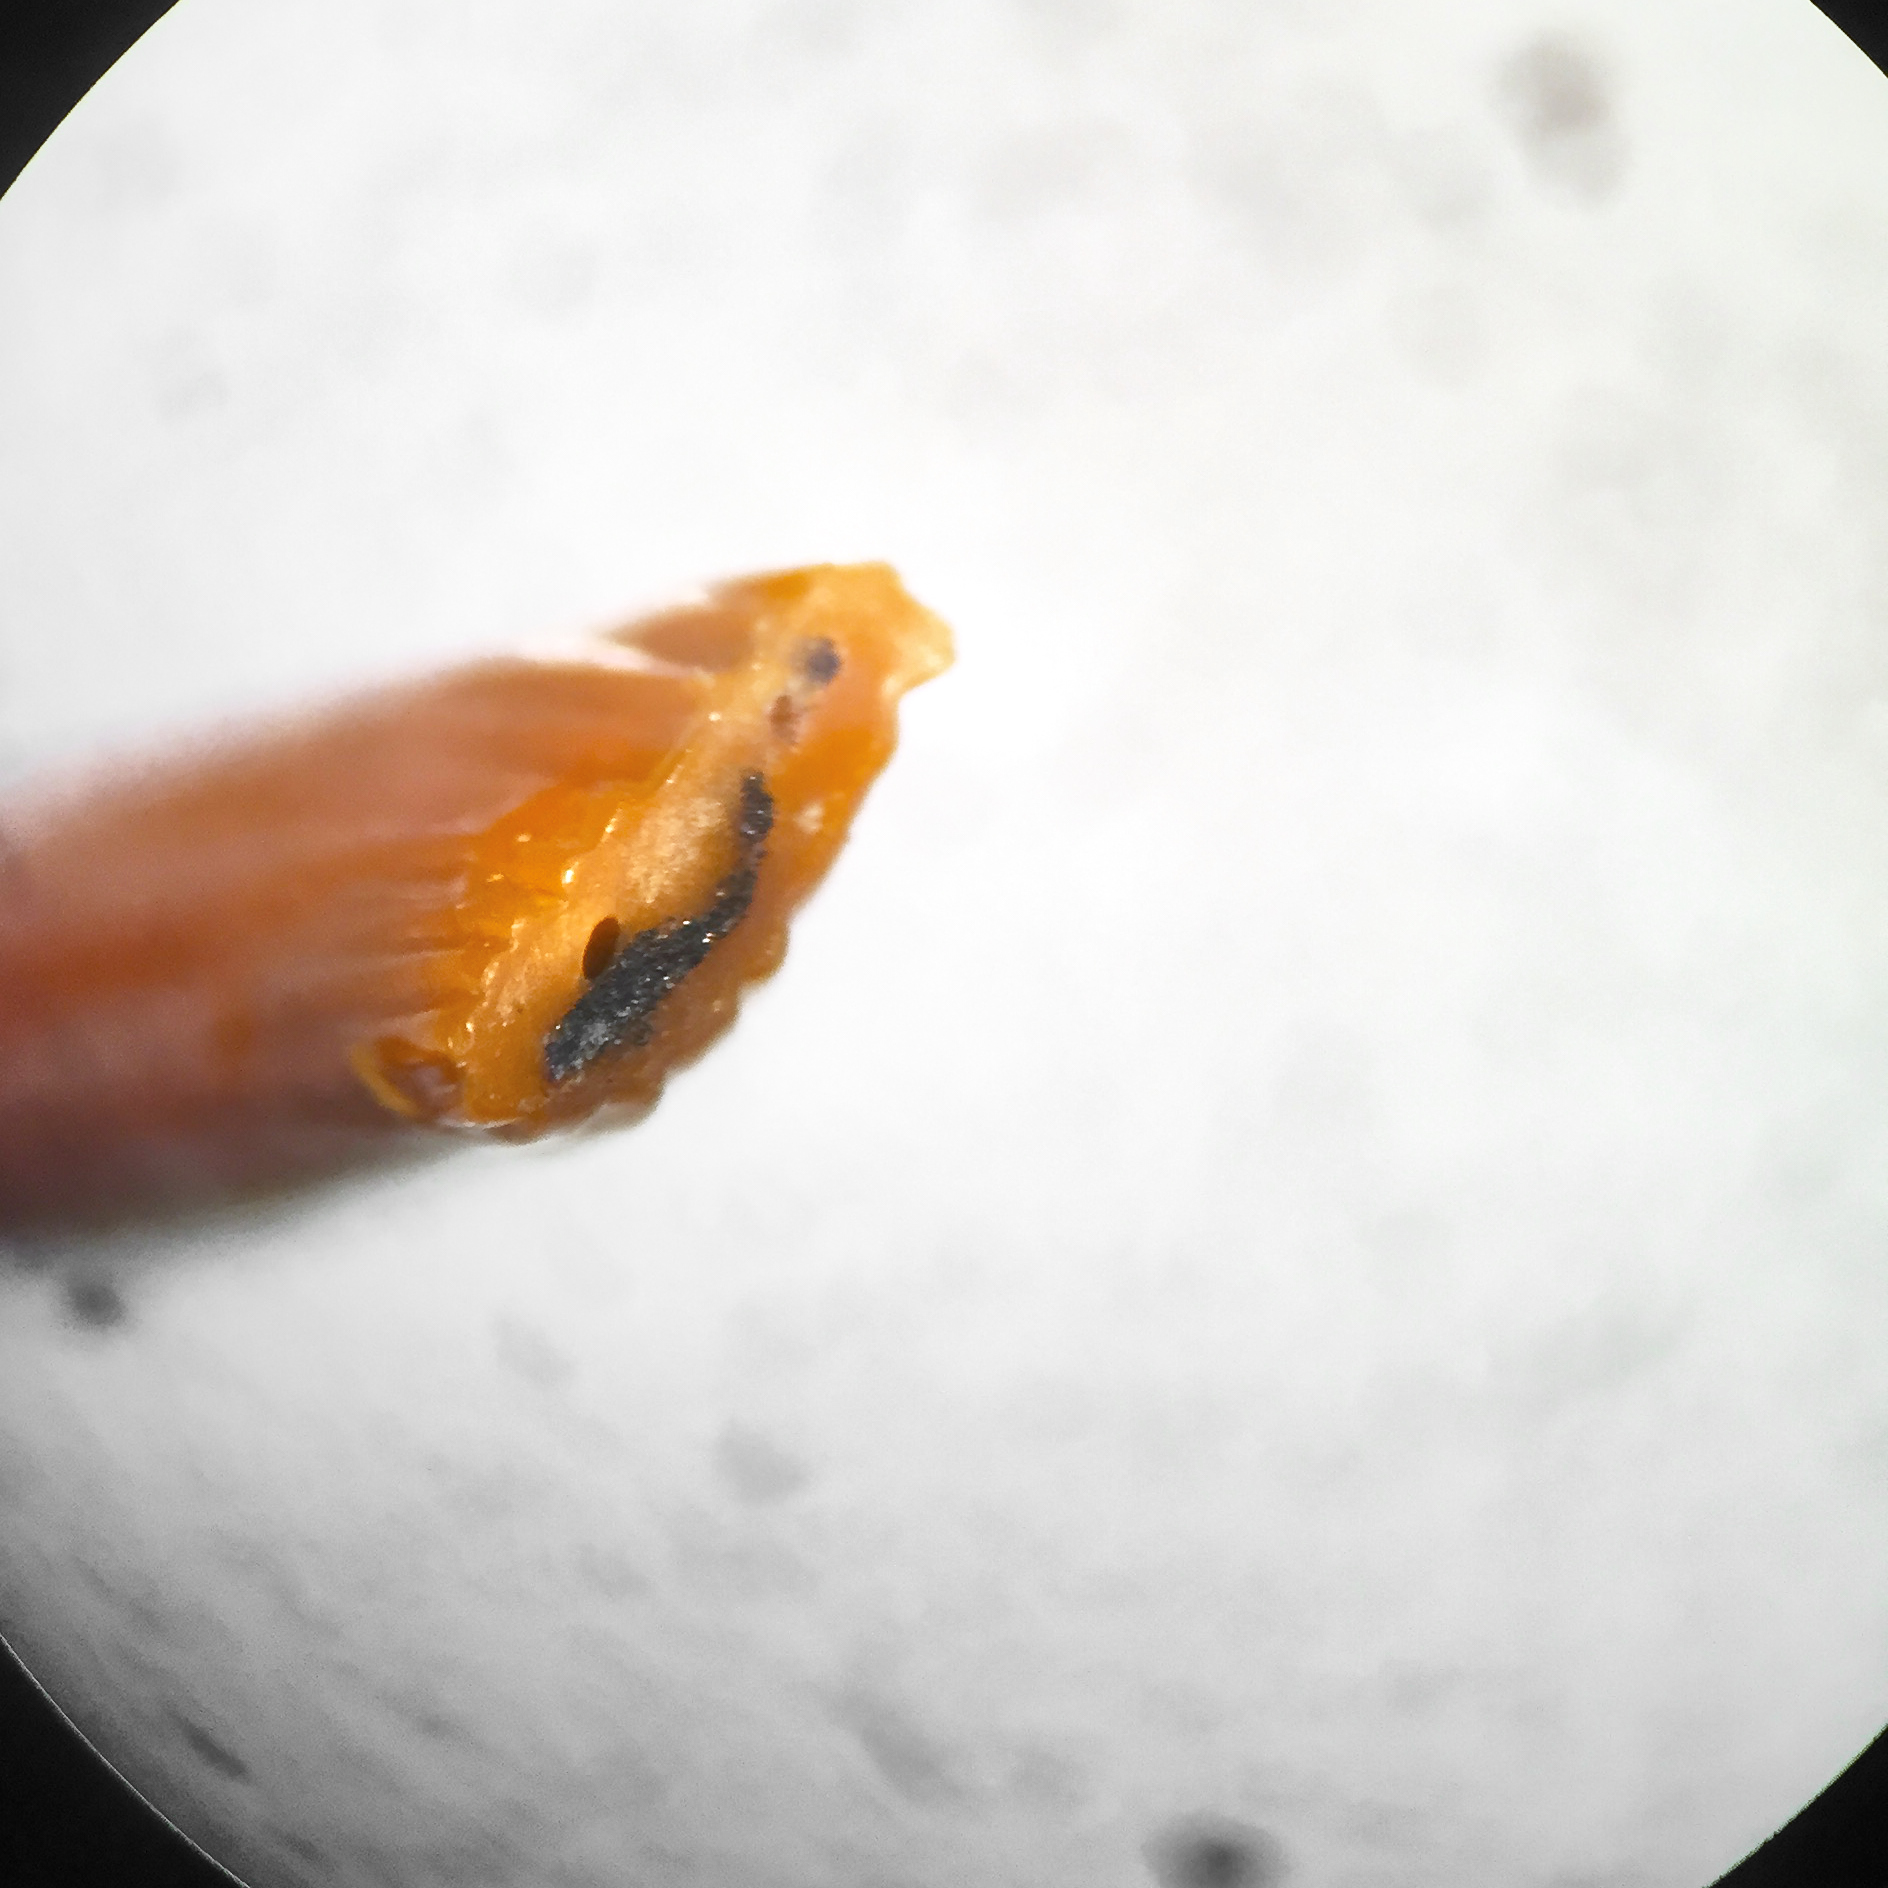
\includegraphics[width=\textwidth]{./figures/filament-108-40-flat-end}
                \caption{Cross section.}
                \label{fig:filament-108-40-flat-end}
        \end{subfigure}
        \caption{Microscopic views (10x) of a CFRP filament created with 5 bathing rotations in a 5\% ABS solution.}\label{fig:filament-108-40-bath-microscope}
\end{figure}


%%% Dipping Results Summary

\begin{table}[h!]
    \centering
    \begin{tabular}{p{1.5in}|p{1in}|p{0.75in}|p{0.75in}|p{0.75in}|p{0.75in}}
        Filament Formulation & Concentration of ABS, $m^3/m^3$ & Density, $kg/m^3$ & Percent Carbon Fiber, $kg/kg$ & Filament Diameter, $mm$ & ABS Added per Dip per Length, $kg/m$  \\ \hline \hline
        60 \textit{in} ABS, 40 \textit{mL} Acetone, Guided & 0.09 & 818 & 19 & 0.73 & 0.017 \\ \hline
        108 \textit{in} ABS, 40 \textit{mL} Acetone, Guided & 0.16 & 758 & 4 & 1.63 & 0.157 \\ \hline
        108 \textit{in} ABS, 40 \textit{mL} Acetone, Bath & 0.16 & 645 & 5 & 1.67 & 0.282 \\
 
    \end{tabular}
    \caption{A summary of dipping results from different slurry concentrations and guide methods.}
    \label{tab:dipping-results}
\end{table}

%%% Dipping Results Discussion

\begin{figure}[htp]
    \centering
    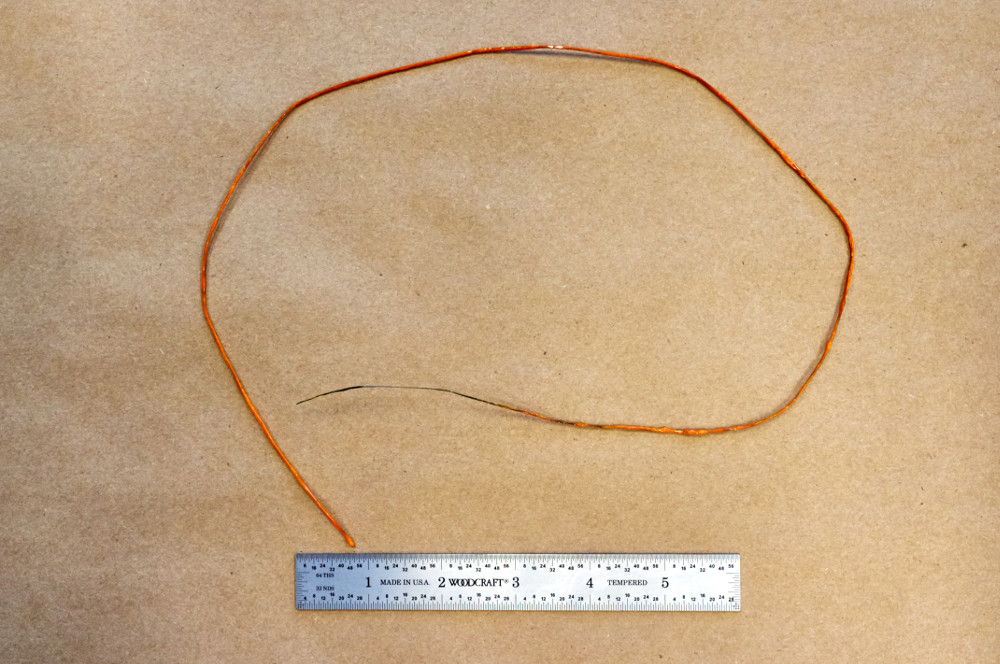
\includegraphics[width=0.8\textwidth]{./figures/filament-dipping-dried}
    \caption{A drying CFRP filament.}
    \label{fig:filament-dipping-dried}
\end{figure}



\begin{figure}[htp]
    \centering
    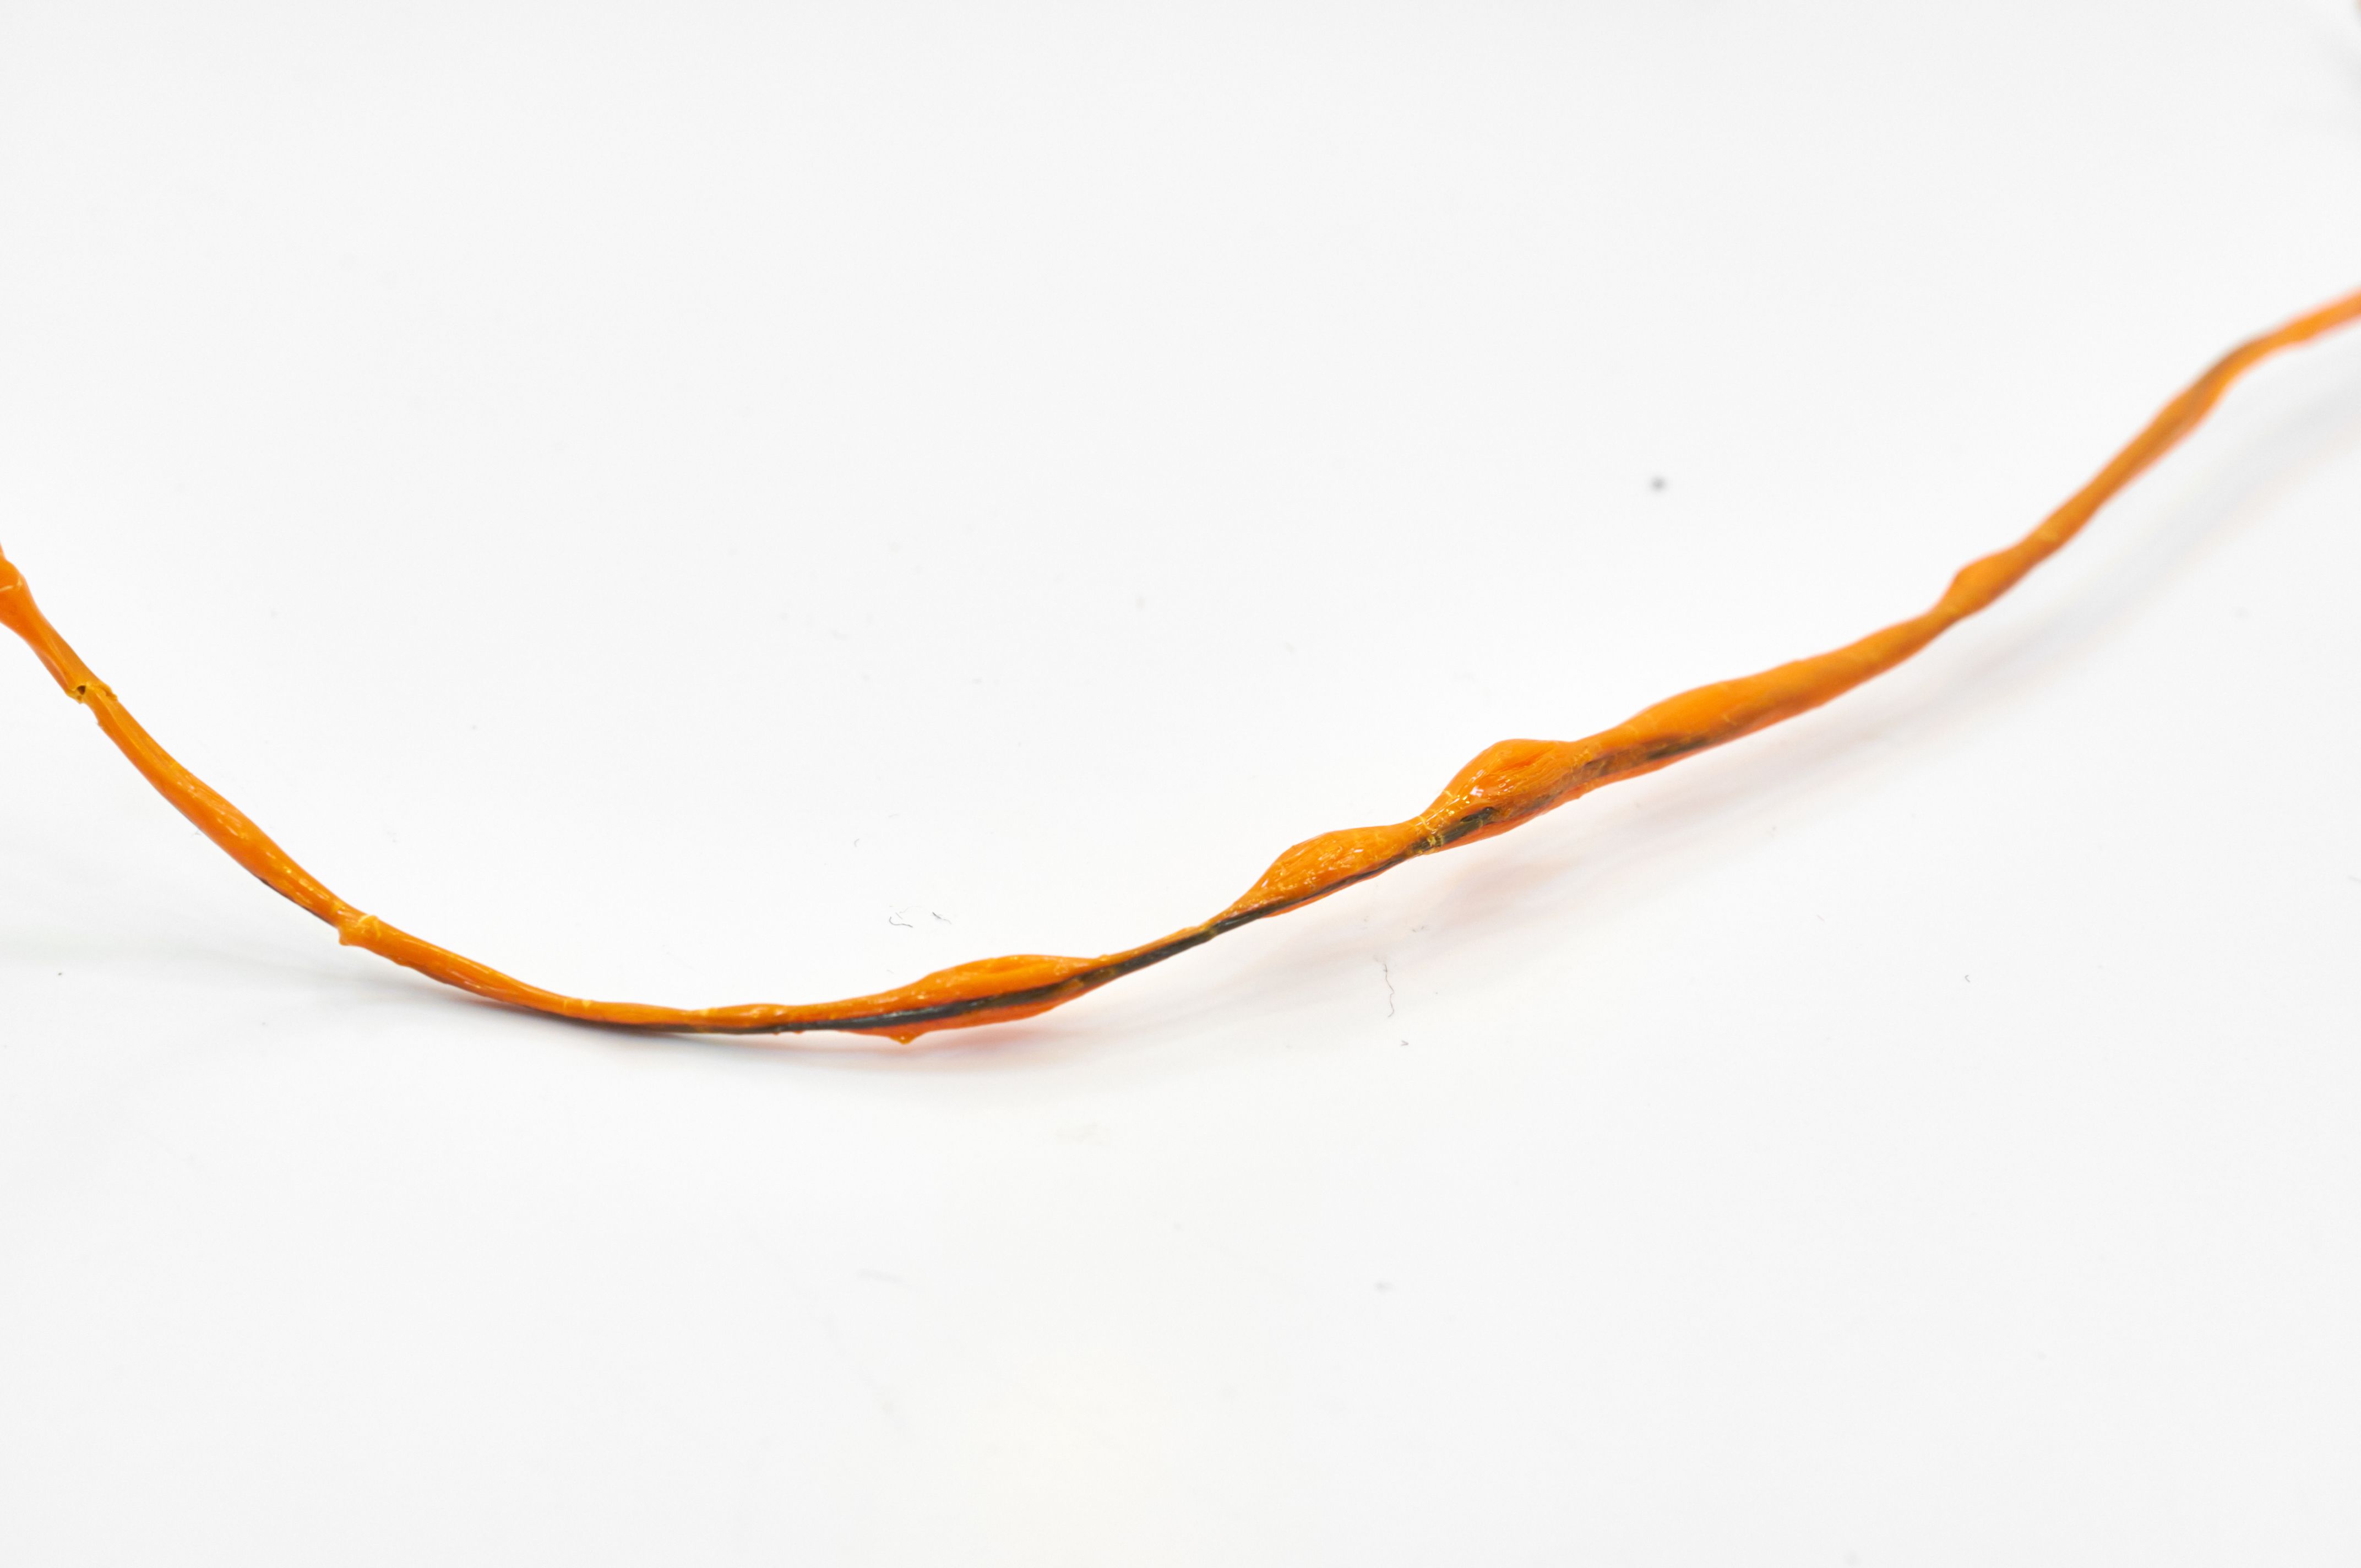
\includegraphics[width=0.8\textwidth]{./figures/filament-dipping-shear}
    \caption{CFRP filament with ABS sheared off from external guides.}
    \label{fig:filament-dipping-shear}
\end{figure}

\clearpage

\subsection{Mechanical Testing}

\indent

\subsubsection{Setup}

\indent

Tensile tests were performed on the filament samples that were produced using the pultrusion and dipping methods. An Instron mechanical testing machine was used for these tests. Short lengths of filament (roughly 2 in) were cut from larger samples for testing. Due to the small, slippery,  and flexible nature of the filament samples, the regular serrated jaw inserts of the Instron tensile test jaws could not be used alone to secure the samples. Instead of clamping the samples directly in the jaws, the samples were securely mounted to aperture cards using melted ABS. The ends of the card were folded over the filament. Once clamped in the serrated jaws, the cardboard protected the filament from the jaws and held it securely in place. The card also assisted in aligning the filament with the jaws. Once clamped, the exposed portion of the card was cut with scissors, and the test was started.\\

\begin{figure}[h!]
    \centering
    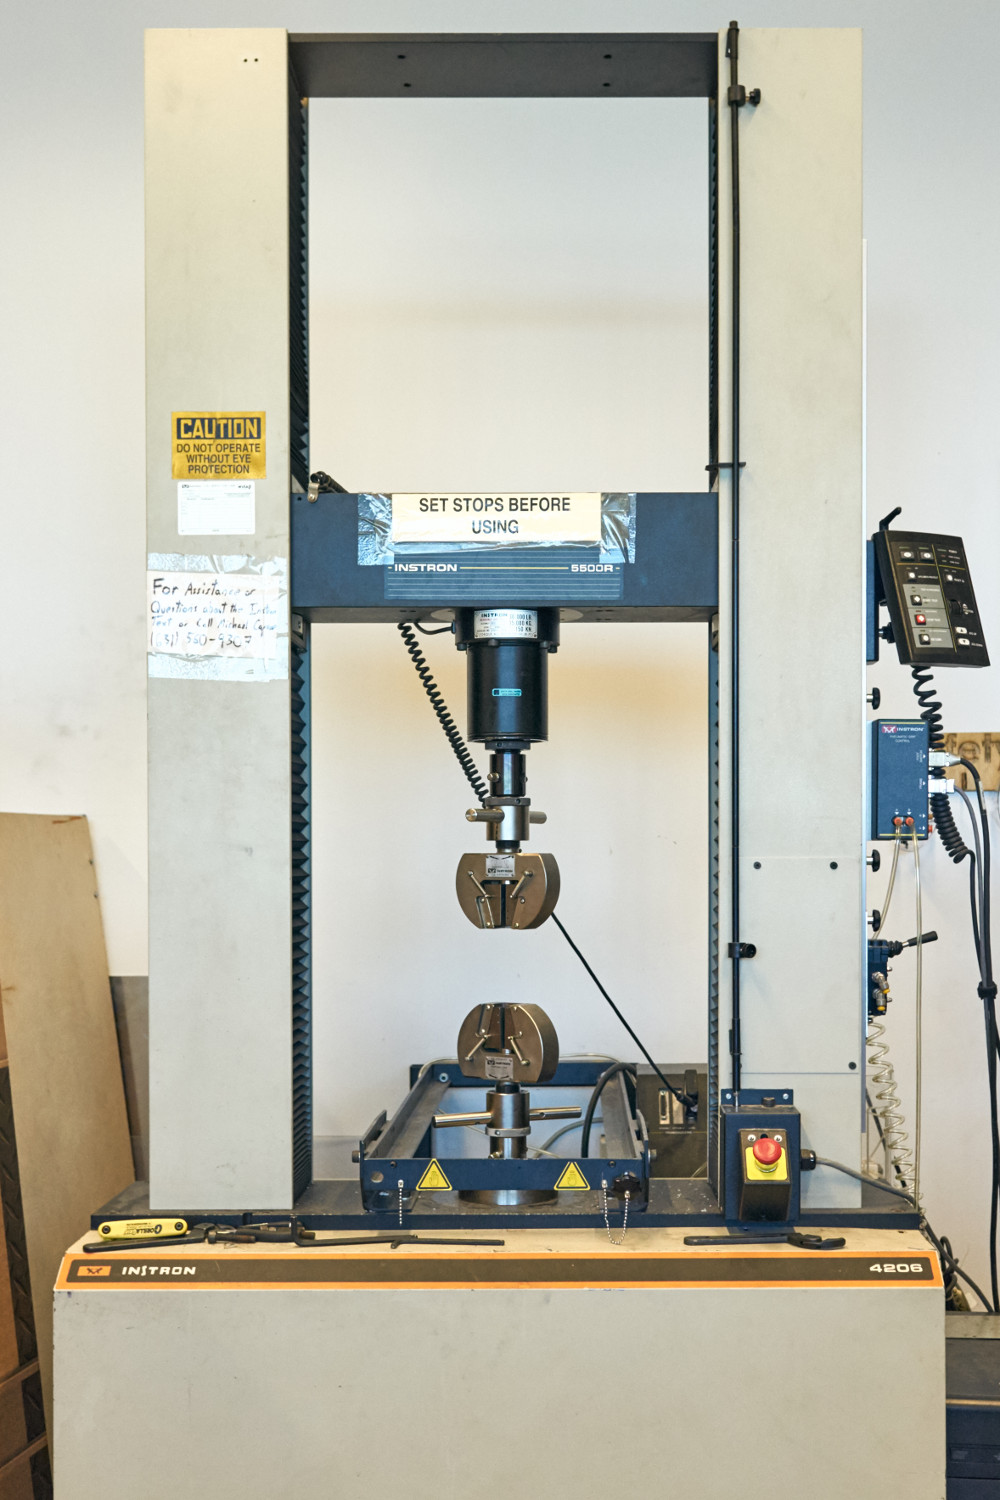
\includegraphics[width=0.5\textwidth]{./figures/intstron-overview}
    \caption{A photo of the Instron machine.}
    \label{fig:intstron-overview}
\end{figure}

\begin{figure}[h!]
        \centering
        \begin{subfigure}[b]{0.3\textwidth}
                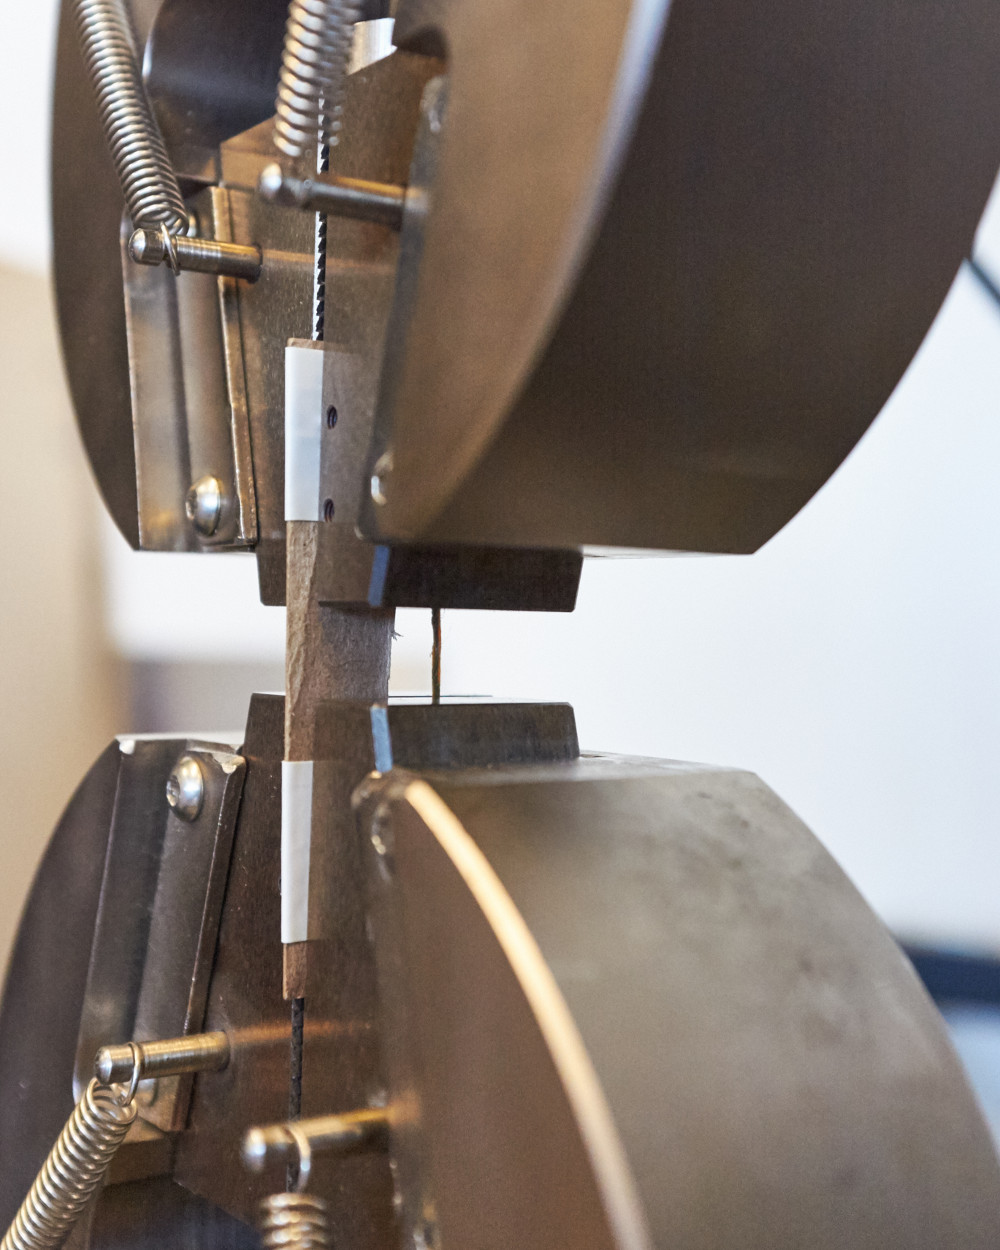
\includegraphics[width=\textwidth]{./figures/filament-instron-1}
                \caption{Installed in jaws.}
                \label{fig:filament-instron-1}
        \end{subfigure}
        \begin{subfigure}[b]{0.3\textwidth}
                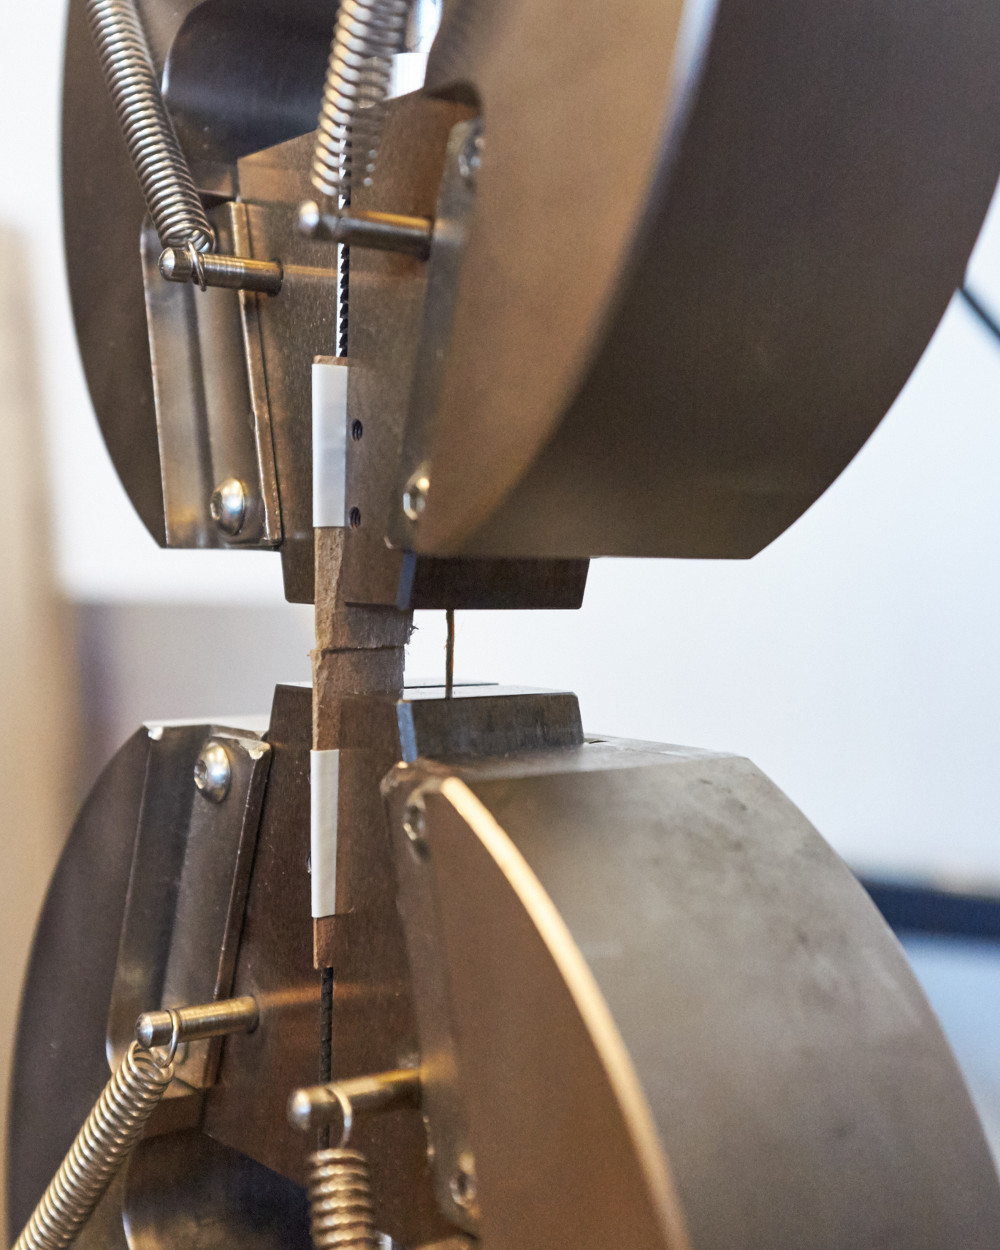
\includegraphics[width=\textwidth]{./figures/filament-instron-2}
                \caption{Cut card ready for testing.}
                \label{fig:filament-instron-2}
        \end{subfigure}
        \caption{A filament specimen loaded in the Instron for a tensile test.}
\end{figure}

\begin{figure}[h!]
    \centering
    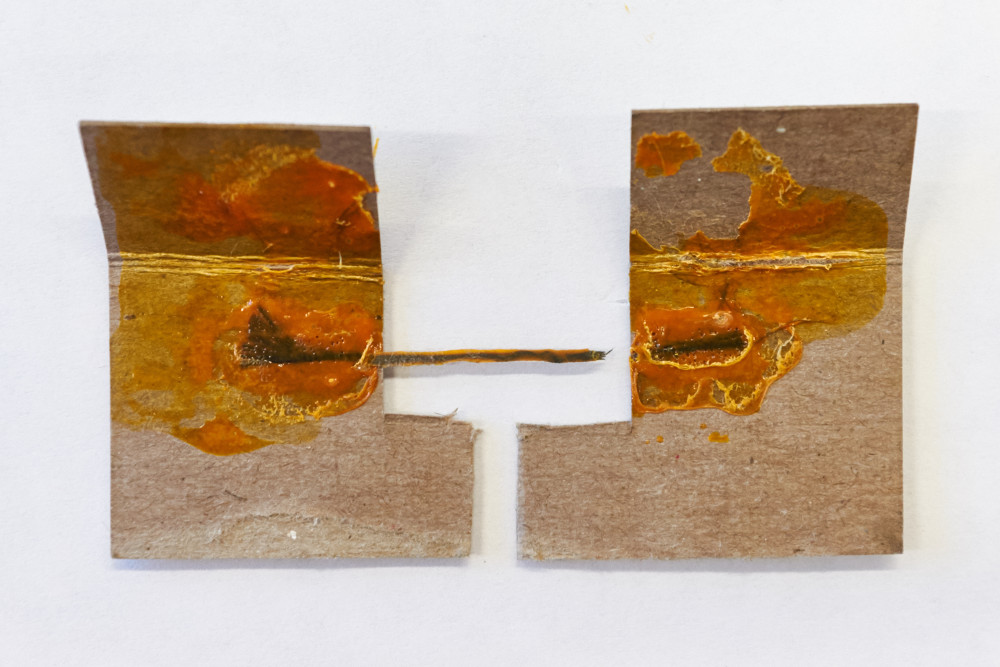
\includegraphics[width=0.5\textwidth]{./figures/filament-card-after-instron}
    \caption{A photo of a filament specimen after tensile testing.}
    \label{fig:filament-card-after-instron}
\end{figure}

\clearpage

\subsubsection{Results}

\indent

The tensile tests performed on the filament samples provide insight into some of their basic mechanical properties. A representative tensile test extension-load plot is provided in Figure~\ref{fig:instron-sample}. The CFRP samples showed fairly linear behavior before failing. Table~\ref{tab:test-results} compares the estimated ultimate tensile strength, stiffness, and density of two\footnote{Nearly a dozen samples were created. These two filaments selected for the table exhibited the most reasonable properties.} filament samples with those of ABS, carbon fiber, and aluminum 6061. The properties of aluminum were included for comparison because CFRP materials are often used to replace aluminum parts. Because it was difficult to consistently clamp the test samples without slipping once the test began, these are only very preliminary results. The results are also affected by inconsistencies in the filament samples themselves. Once the filament production method and test setup are further refined for consistency, further tests will be done to better characterize the properties of the filament. For now, however, the results are promising: both the pultruded and dipped filament samples are lighter and have a higher ultimate tensile strength than aluminum 6061, although they are not as stiff.\\

\begin{figure}[htp]
    \centering
    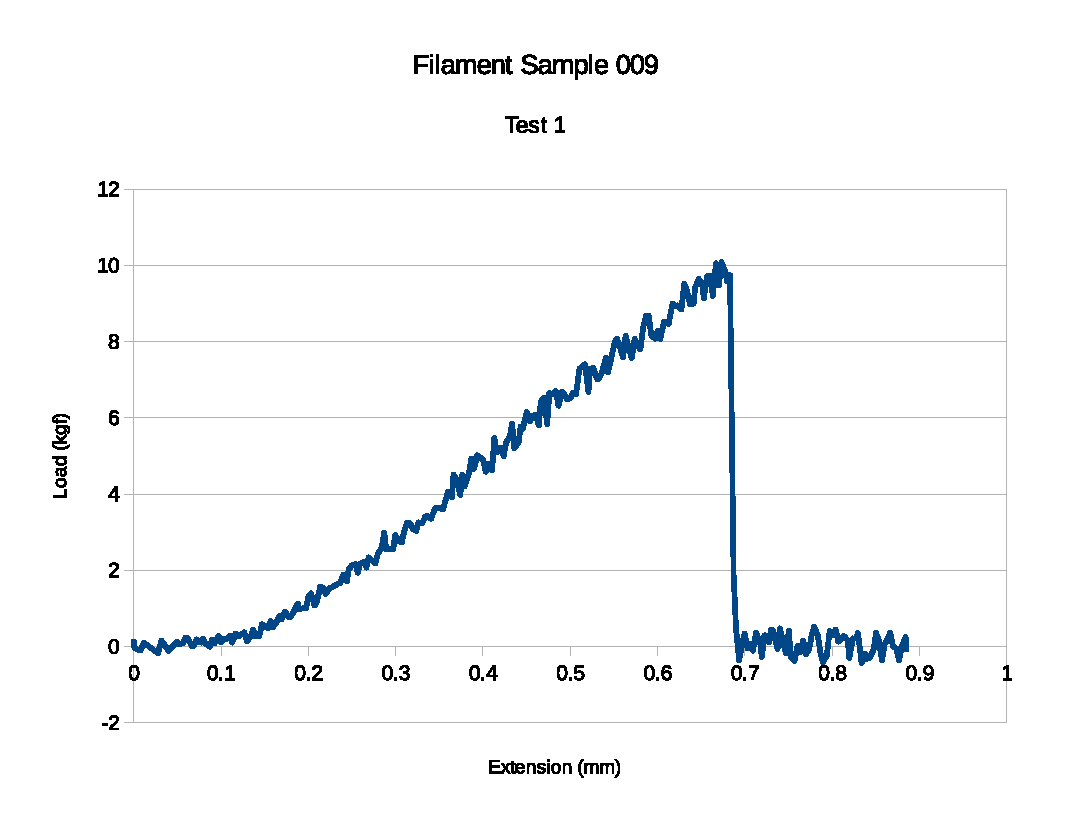
\includegraphics[width=0.8\textwidth]{./figures/009T1-instron-data}
    \caption{Sample tensile test data for a slurry-dipped filament sample.}
    \label{fig:instron-sample}
\end{figure}

\begin{table}[h]
    \centering
    \begin{tabular}{lcccc}
        Material           & Ultimate Tensile Strength (MPa)   & Stiffness (GPa)    & Density ($ kg/m^{3} $)  \\ \hline
        ABS                & 53                                & 2.3                & 1040 \\
        Carbon Fiber       & 3750                              & 231                & 1750 \\
        Aluminum 6061      & 310                               & 68.9               & 2700 \\
        Pultruded Filament & 313                               & 13.4               & 1354 \\ 
        Dipped Filament    & 690                               & 19.6               & 1567 \\
    \end{tabular}
    \caption{Preliminary CFRP filament test results, as compared to its constituents and to aluminum.}
    \label{tab:test-results}
\end{table}

\clearpage

\subsection{Print Testing}

\indent

\begin{figure}[h!]
        \centering
        \begin{subfigure}[b]{0.3\textwidth}
                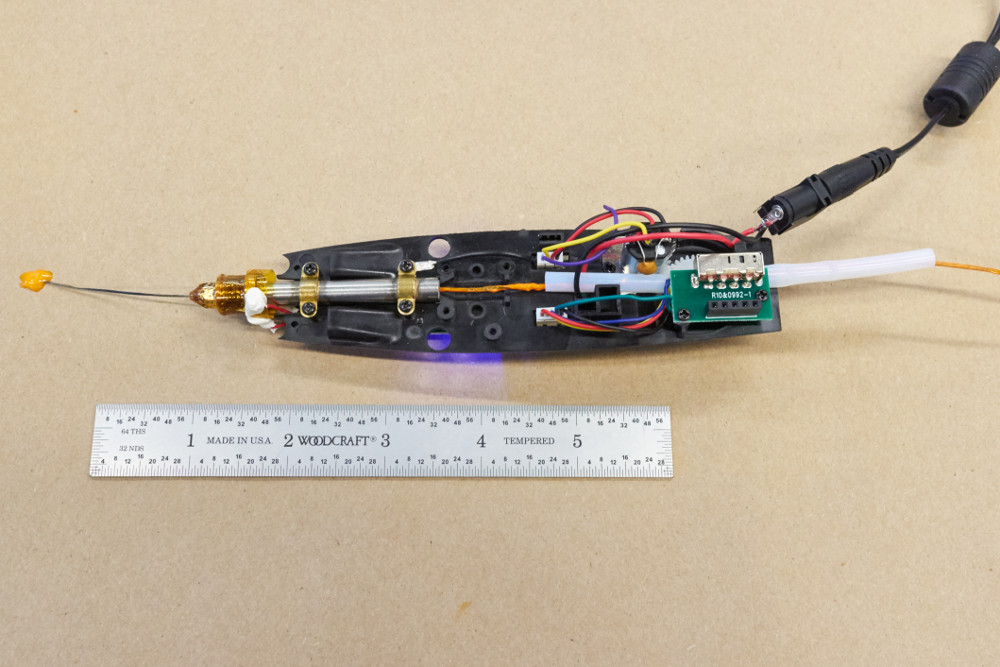
\includegraphics[width=\textwidth]{./figures/filament-print-3doodler-before}
                \caption{Before.}
                \label{fig:filament-print-3doodler-before}
        \end{subfigure}
        \begin{subfigure}[b]{0.3\textwidth}
                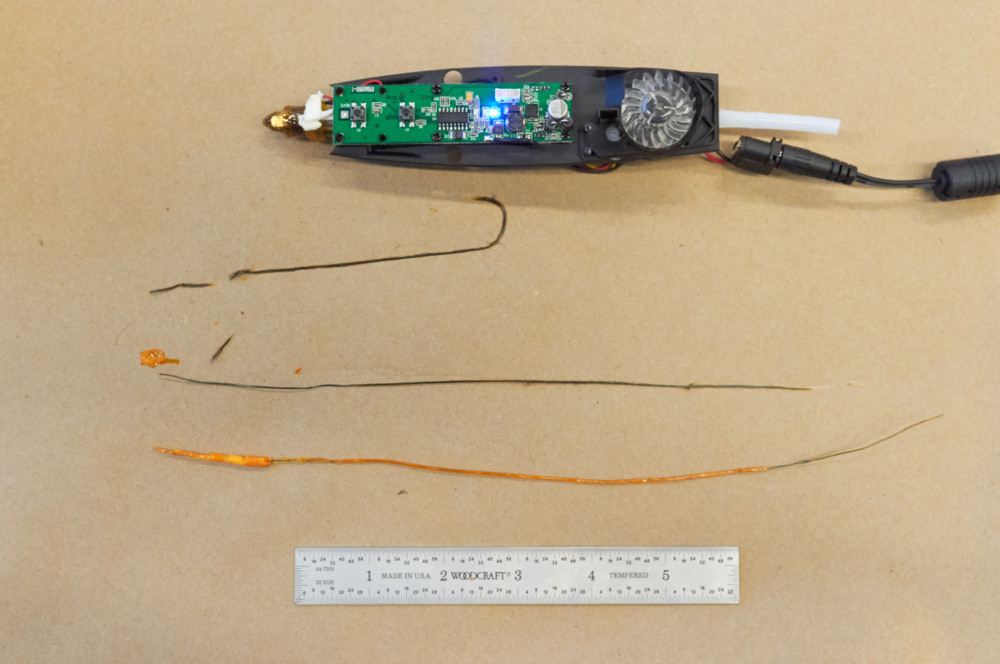
\includegraphics[width=\textwidth]{./figures/filament-print-3doodler-after}
                \caption{After.}
                \label{fig:filament-print-3doodler-after}
        \end{subfigure}
        \caption{Before and after shots of print testing with the CFRP filament.}\label{fig:filament-print-test}
\end{figure}

\begin{figure}[htp]
    \centering
    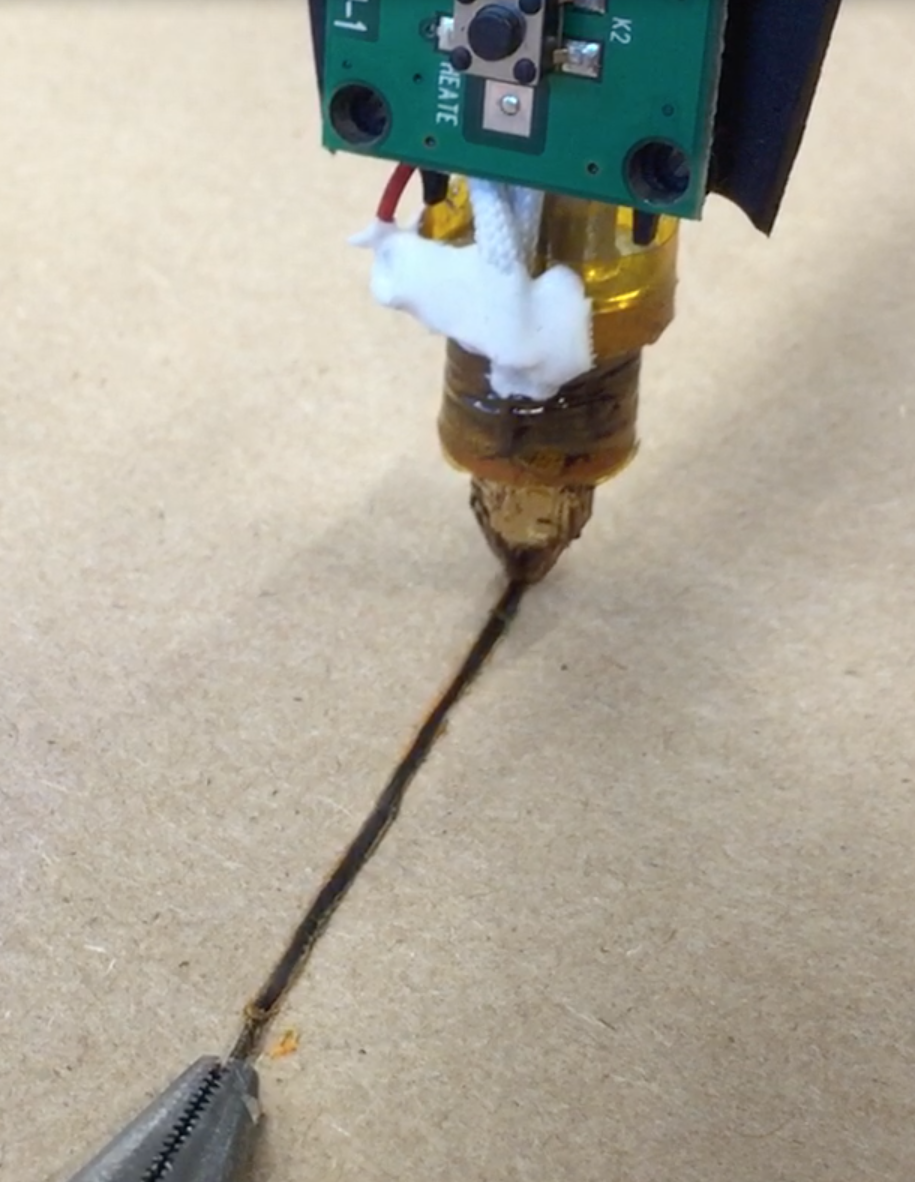
\includegraphics[width=0.5\textwidth]{./figures/filament-print-3doodler-during}
    \caption{Test printing the CFRP filament with a 3Doodler.}
    \label{fig:filament-print-3doodler-during}
\end{figure}

\begin{figure}[htp]
    \centering
    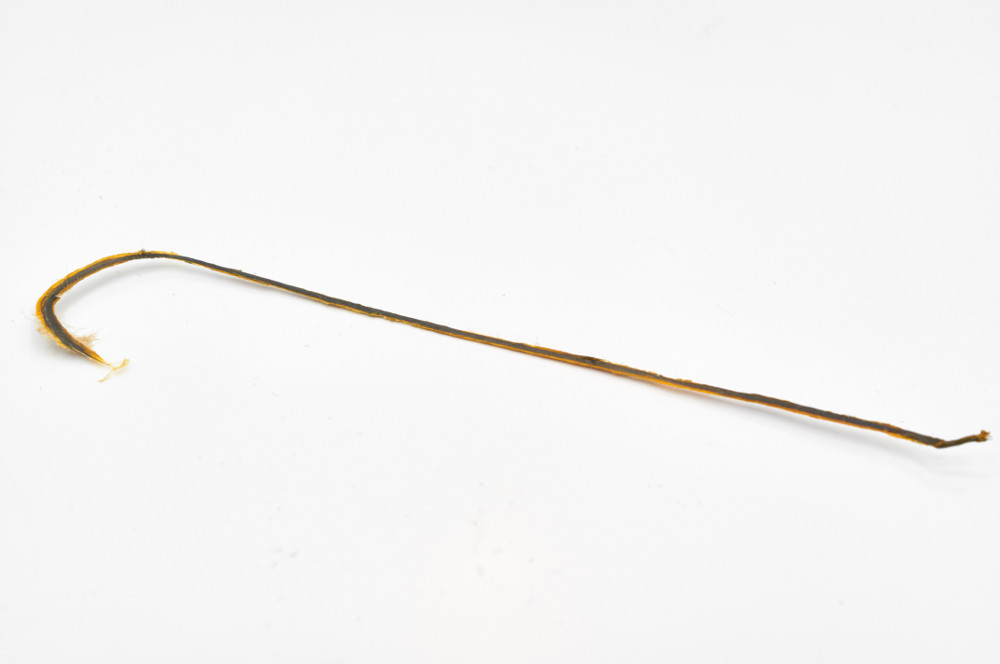
\includegraphics[width=0.8\textwidth]{./figures/filament-extrude}
    \caption{A close up photo of the filament printed with the 3Doodler}
    \label{fig:filament-extrude}
\end{figure}

\begin{table}[h]
    \centering
    \begin{tabular}{lcccc}
        Material           & Ultimate Tensile Strength (MPa)   & Stiffness (GPa)    & Failure Strain (\%)  \\ \hline
		Printed Filament & 338 & 7.63 & 4.44
    \end{tabular}
    \caption{Tensile test results for the printed CFRP filament}
    \label{tab:printed-filament-results}
\end{table}

\subsection{Future Suggestions}

%research and methods

\clearpage

%----------------------------------------------------------
\section{Material Analysis}

\indent

Material analysis will be performed on the printed CFRP parts. Part geometry will be chosen such that CFRP curved layer, ABS curved layer, and ABS cartesian layer parts can be printed for comparison. Specific to part geometries, the Instron Tension Tester will be used to implement bending, compression and tensile tests as appropriate to quantify the strength and stiffness of each print. Strain gauges may even be placed along exposed fibers in attempt to determine fiber-specific stresses and strains.\\

% experimental stuff we haven't gotten to yet

\clearpage

%----------------------------------------------------------
\section{Fiber Orientation Optimization}

\indent

CFRPs exhibit maximum strength when fibers align appropriately with the loads. Therefore, fiber orientation within parts is critical. Finite element analysis software will be utilized to determine optimal fiber orientation and printing tool paths will be generated from this data.

\subsection{Finite Element Analysis}

\indent

\emph{ANSYS} finite element software will be used to determine fiber orientation within printed parts. The \emph{Composite PrepPost} package, which is specifically designed to assess the strength of composite structures, will be used. The package utilizes shell elements that contain matrix and fiber material properties. The software also contains multiple laminate failure criteria and can perform optimization loops to determine the strongest configuration of fiber angles. For instance, a tube can discretized into a number of shell elements, assigned a number of layers, given isotropic matrix material properties and orthotropic fiber material properties, and iterated through different fiber angles to calculate stress and deformation gradients across the entire part (at all angles or at only the strongest angle). Therefore, once the specific printed part geometry for the curved layer carbon fiber is determined, this software will be used to find optimal fiber orientation(s).\footnote{Dr. Wootton has advised that many computation analyses usually overshoot experimental strength results. However, experimental and theoretical results will typically agree in trends and the computational model will sufficiently locate the weakest area(s) of the geometry.}\\

\subsubsection{Geometry}

insert geometry stuff here

\subsubsection{Loading and Boundary Conditions}

insert loading stuff here

\subsubsection{Meshing}

insert meshing stuff here

\subsubsection{ACP Setup}

insert acp setup specific stuff here

\subsubsection{ACP Results}

insert acp results here

\subsubsection{Solid Body FEA Comparison}

insert abs and al solid body fea here

\subsubsection{Conclusions from FEA}

insert conclusions / future suggestions here

\subsection{Toolpath Generation}

\indent

The toolpath for an FDM 3D printer is the path in space that the extruder follows while it prints a part. In most FDM printers, the toolpath is sent to the machine in a machine control language known as Gcode. Many existing programs, open source and proprietary, can be used to turn an STL file into Gcode. Because current 3D printers all use flat layers, these slicing programs are not suitable for creating curved-layer toolpaths. Fortunately, parts of some modular open source slicing programs may be repurposed for generating curved layer toolpaths. Once the toolpaths are generated, they will be converted to TP (FANUC's robot control language) and sent to the FANUC robot controller. \\


%ansys and whatnot

\clearpage

%-----------------------------------------------------------
%\input{next-steps.tex}
%
%\clearpage

%-----------------------------------------------------------
\section{Conclusion}

A curved-layer CFRP 3D printer is under development to print parts with greater strength than current FDM printers. With curved layers, the carbon fiber may be oriented to best suit the applied loading on any given part, and the layers may be designed for greater inter-layer adhesion. An FDM-compatible ABS-matrix CFRP filament was developed and shown to have promising mechanical properties, comparable to aluminum. A custom FDM extruder was designed and prototyped for mounting on an available FANUC industrial robot arm, which provides the six necessary degrees of freedom to print curved layers. Control electronics were assembled and will be programmed to control the custom extruder and take input signals from the FANUC robot controller. A composite-specific finite element analysis software package was acquired and will be used to optimize the print layer geometry. Future work includes manufacturing the custom extruder; refining the filament production and test methods to create a printable CFRP; programming the robot and extruder controller; generating optimized layer geometries; and printing and testing the CFRP material. 



\clearpage

%----------------------------------------------------------
\section{Acknowledgements}

\indent

First and foremost we wish to thank our advisor Dr. Stan Wei for his guidance on this project and for providing us access to the FANUC robot arm. We also wish to thank Dr. David Wootton and Dr. Eric Lima for providing specifc advise related to material analysis while we were developing our filament as well as general intermittent guidance. Brian Yudin and Estuardo Rodas deserve thanks for their guidance pertaining to the mechanical design of the extruder and their assistance in locating hardware required for electrical fixturing. Dr. Scott Bondi also deserves to be thanked for his assistance in locating a viable finite element software package for analyzing composites, as well as providing initial guidance on how to use the software. Finally, we would like to acknowledge Keith Ng for obtaining and installing \emph{ANSYS Composite PrepPost} on all computer center computers.

% Wei, Wootton, Brian, Scondi, Keith, Lima, Estuardo

\clearpage

%----------------------------------------------------------
%\section{Bibliography}

\bibliographystyle{plain}
\bibliography{pj-sem1}

% how do you bibtex across multiple input files?

\clearpage

%----------------------------------------------------------
%\input{appendix-1.tex}
%
%\clearpage

%----------------------------------------------------------
%\input{appendix-1.tex}
%
%\clearpage


\end{document}
